\documentclass[letterpaper]{article}
\usepackage[top=1in,left=1in,bottom=1in,right=1in]{geometry}
\usepackage{makeidx}
\usepackage{natbib}
\usepackage{graphicx}
\usepackage{multicol}
\usepackage{float}
\usepackage{listings}
\usepackage{color}
\usepackage{ifthen}
\usepackage[table]{xcolor}
\usepackage{textcomp}
\usepackage{alltt}
\usepackage{ifpdf}
\ifpdf
\usepackage[pdftex,
            pagebackref=true,
            colorlinks=true,
            linkcolor=blue,
            unicode
           ]{hyperref}
\else
\usepackage[ps2pdf,
            pagebackref=true,
            colorlinks=true,
            linkcolor=blue,
            unicode
           ]{hyperref}
\usepackage{pspicture}
\fi
\usepackage[utf8]{inputenc}
\usepackage{mathptmx}
\usepackage[scaled=.90]{helvet}
\usepackage{courier}
\usepackage{sectsty}
\usepackage[titles]{tocloft}
\usepackage{doxygen}
\lstset{language=C++,inputencoding=utf8,basicstyle=\footnotesize,breaklines=true,breakatwhitespace=true,tabsize=8,numbers=left }
\makeindex
\setcounter{tocdepth}{3}
\renewcommand{\familydefault}{\sfdefault}
\hfuzz=15pt
\setlength{\emergencystretch}{15pt}
\hbadness=750
\tolerance=750
\begin{document}
\hypersetup{pageanchor=false,citecolor=blue}
\begin{titlepage}
\vspace*{1cm}
\begin{center}

{\Large ForceBalance Developer API Guide version 1.2}\\
\vspace*{2cm}
{\large Generated by Doxygen 1.7.6.1}\\
\vspace*{2.5 cm}

\includegraphics[width=3in]{ForceBalance}
\end{center}
\end{titlepage}
\pagenumbering{roman}
\tableofcontents
\pagenumbering{arabic}
\hypersetup{pageanchor=true,citecolor=blue}
\section{Project Roadmap}
\label{roadmap}
\hypertarget{roadmap}{}
Force\-Balance is a work in progress and is continually being improved and expanded! Here are some current and future project development ideas.\hypertarget{roadmap_summer}{}\subsection{Short Term (summer 2013)}\label{roadmap_summer}
\begin{DoxyItemize}
\item Create and expand project unit testing framework to encourage a test driven development approach \item Improve/consolidate existing documentation\end{DoxyItemize}
\hypertarget{roadmap_longterm}{}\subsection{Long Term}\label{roadmap_longterm}
\begin{DoxyItemize}
\item Development of a Force\-Balance G\-U\-I interface to complement the current command line interface \item More comprehensive tutorial to walk users through the initial process of setting up targets and preparing for a successful Force\-Balance run \end{DoxyItemize}

\section{Namespace Index}
\subsection{Packages}
Here are the packages with brief descriptions (if available)\+:\begin{DoxyCompactList}
\item\contentsline{section}{\hyperlink{namespacefilecnv}{filecnv} }{\pageref{namespacefilecnv}}{}
\item\contentsline{section}{\hyperlink{namespaceforcebalance}{forcebalance} }{\pageref{namespaceforcebalance}}{}
\item\contentsline{section}{\hyperlink{namespaceForceBalance}{Force\+Balance} \\*Executable script for starting \hyperlink{namespaceForceBalance}{Force\+Balance} }{\pageref{namespaceForceBalance}}{}
\item\contentsline{section}{\hyperlink{namespaceforcebalance_1_1abinitio}{forcebalance.\+abinitio} \\*Ab-\/initio fitting module (energies, forces, resp) }{\pageref{namespaceforcebalance_1_1abinitio}}{}
\item\contentsline{section}{\hyperlink{namespaceforcebalance_1_1abinitio__internal}{forcebalance.\+abinitio\+\_\+internal} \\*Internal implementation of energy matching (for T\+I\+P3P water only) }{\pageref{namespaceforcebalance_1_1abinitio__internal}}{}
\item\contentsline{section}{\hyperlink{namespaceforcebalance_1_1amberio}{forcebalance.\+amberio} \\*A\+M\+B\+ER force field input/output }{\pageref{namespaceforcebalance_1_1amberio}}{}
\item\contentsline{section}{\hyperlink{namespaceforcebalance_1_1binding}{forcebalance.\+binding} \\*Binding energy fitting module }{\pageref{namespaceforcebalance_1_1binding}}{}
\item\contentsline{section}{\hyperlink{namespaceforcebalance_1_1counterpoise}{forcebalance.\+counterpoise} \\*Match an empirical potential to the counterpoise correction for basis set superposition error (B\+S\+SE) }{\pageref{namespaceforcebalance_1_1counterpoise}}{}
\item\contentsline{section}{\hyperlink{namespaceforcebalance_1_1custom__io}{forcebalance.\+custom\+\_\+io} \\*Custom force field parser }{\pageref{namespaceforcebalance_1_1custom__io}}{}
\item\contentsline{section}{\hyperlink{namespaceforcebalance_1_1evaluator}{forcebalance.\+evaluator} \\*A target which employs the Open\+FF Evaluator framework to compute condensed phase physical properties }{\pageref{namespaceforcebalance_1_1evaluator}}{}
\item\contentsline{section}{\hyperlink{namespaceforcebalance_1_1forcefield}{forcebalance.\+forcefield} \\*Force field module }{\pageref{namespaceforcebalance_1_1forcefield}}{}
\item\contentsline{section}{\hyperlink{namespaceforcebalance_1_1gmxio}{forcebalance.\+gmxio} \\*G\+R\+O\+M\+A\+CS input/output }{\pageref{namespaceforcebalance_1_1gmxio}}{}
\item\contentsline{section}{\hyperlink{namespaceforcebalance_1_1hydration}{forcebalance.\+hydration} \\*Hydration free energy fitting module }{\pageref{namespaceforcebalance_1_1hydration}}{}
\item\contentsline{section}{\hyperlink{namespaceforcebalance_1_1interaction}{forcebalance.\+interaction} \\*Interaction energy fitting module }{\pageref{namespaceforcebalance_1_1interaction}}{}
\item\contentsline{section}{\hyperlink{namespaceforcebalance_1_1lipid}{forcebalance.\+lipid} \\*Matching of lipid bulk properties }{\pageref{namespaceforcebalance_1_1lipid}}{}
\item\contentsline{section}{\hyperlink{namespaceforcebalance_1_1liquid}{forcebalance.\+liquid} \\*Matching of liquid bulk properties }{\pageref{namespaceforcebalance_1_1liquid}}{}
\item\contentsline{section}{\hyperlink{namespaceforcebalance_1_1moments}{forcebalance.\+moments} \\*Multipole moment fitting module }{\pageref{namespaceforcebalance_1_1moments}}{}
\item\contentsline{section}{\hyperlink{namespaceforcebalance_1_1nifty}{forcebalance.\+nifty} \\*Nifty functions, intended to be imported by any module within \hyperlink{namespaceForceBalance}{Force\+Balance} }{\pageref{namespaceforcebalance_1_1nifty}}{}
\item\contentsline{section}{\hyperlink{namespaceforcebalance_1_1objective}{forcebalance.\+objective} \\*\hyperlink{namespaceForceBalance}{Force\+Balance} objective function }{\pageref{namespaceforcebalance_1_1objective}}{}
\item\contentsline{section}{\hyperlink{namespaceforcebalance_1_1openmmio}{forcebalance.\+openmmio} \\*Open\+MM input/output }{\pageref{namespaceforcebalance_1_1openmmio}}{}
\item\contentsline{section}{\hyperlink{namespaceforcebalance_1_1opt__geo__target}{forcebalance.\+opt\+\_\+geo\+\_\+target} \\*Optimized Geometry fitting module }{\pageref{namespaceforcebalance_1_1opt__geo__target}}{}
\item\contentsline{section}{\hyperlink{namespaceforcebalance_1_1optimizer}{forcebalance.\+optimizer} \\*Optimization algorithms }{\pageref{namespaceforcebalance_1_1optimizer}}{}
\item\contentsline{section}{\hyperlink{namespaceforcebalance_1_1parser}{forcebalance.\+parser} \\*Input file parser for \hyperlink{namespaceForceBalance}{Force\+Balance} jobs }{\pageref{namespaceforcebalance_1_1parser}}{}
\item\contentsline{section}{\hyperlink{namespaceforcebalance_1_1psi4io}{forcebalance.\+psi4io} \\*P\+S\+I4 force field input/output }{\pageref{namespaceforcebalance_1_1psi4io}}{}
\item\contentsline{section}{\hyperlink{namespaceforcebalance_1_1qchemio}{forcebalance.\+qchemio} \\*Q-\/\+Chem input file parser }{\pageref{namespaceforcebalance_1_1qchemio}}{}
\item\contentsline{section}{\hyperlink{namespaceforcebalance_1_1smirnoff}{forcebalance.\+smirnoff} \\*S\+M\+I\+R\+N\+O\+FF force field support }{\pageref{namespaceforcebalance_1_1smirnoff}}{}
\item\contentsline{section}{\hyperlink{namespaceforcebalance_1_1tinkerio}{forcebalance.\+tinkerio} \\*T\+I\+N\+K\+ER input/output }{\pageref{namespaceforcebalance_1_1tinkerio}}{}
\item\contentsline{section}{\hyperlink{namespaceforcebalance_1_1torsion__profile}{forcebalance.\+torsion\+\_\+profile} \\*Torsion profile fitting module }{\pageref{namespaceforcebalance_1_1torsion__profile}}{}
\item\contentsline{section}{\hyperlink{namespaceforcebalance_1_1vibration}{forcebalance.\+vibration} \\*Vibrational mode fitting module }{\pageref{namespaceforcebalance_1_1vibration}}{}
\item\contentsline{section}{\hyperlink{namespaceMakeInputFile}{Make\+Input\+File} \\*Executable script for printing out an example input file with defaults and documentation }{\pageref{namespaceMakeInputFile}}{}
\item\contentsline{section}{\hyperlink{namespacesrc}{src} }{\pageref{namespacesrc}}{}
\item\contentsline{section}{\hyperlink{namespacesrc_1_1__version}{src.\+\_\+version} }{\pageref{namespacesrc_1_1__version}}{}
\item\contentsline{section}{\hyperlink{namespacesrc_1_1abinitio}{src.\+abinitio} }{\pageref{namespacesrc_1_1abinitio}}{}
\item\contentsline{section}{\hyperlink{namespacesrc_1_1abinitio__internal}{src.\+abinitio\+\_\+internal} }{\pageref{namespacesrc_1_1abinitio__internal}}{}
\item\contentsline{section}{\hyperlink{namespacesrc_1_1amberio}{src.\+amberio} }{\pageref{namespacesrc_1_1amberio}}{}
\item\contentsline{section}{\hyperlink{namespacesrc_1_1binding}{src.\+binding} }{\pageref{namespacesrc_1_1binding}}{}
\item\contentsline{section}{\hyperlink{namespacesrc_1_1chemistry}{src.\+chemistry} }{\pageref{namespacesrc_1_1chemistry}}{}
\item\contentsline{section}{\hyperlink{namespacesrc_1_1counterpoise}{src.\+counterpoise} }{\pageref{namespacesrc_1_1counterpoise}}{}
\item\contentsline{section}{\hyperlink{namespacesrc_1_1custom__io}{src.\+custom\+\_\+io} }{\pageref{namespacesrc_1_1custom__io}}{}
\item\contentsline{section}{\hyperlink{namespacesrc_1_1engine}{src.\+engine} }{\pageref{namespacesrc_1_1engine}}{}
\item\contentsline{section}{\hyperlink{namespacesrc_1_1evaluator__io}{src.\+evaluator\+\_\+io} }{\pageref{namespacesrc_1_1evaluator__io}}{}
\item\contentsline{section}{\hyperlink{namespacesrc_1_1ffyapf}{src.\+ffyapf} }{\pageref{namespacesrc_1_1ffyapf}}{}
\item\contentsline{section}{\hyperlink{namespacesrc_1_1finite__difference}{src.\+finite\+\_\+difference} }{\pageref{namespacesrc_1_1finite__difference}}{}
\item\contentsline{section}{\hyperlink{namespacesrc_1_1forcefield}{src.\+forcefield} }{\pageref{namespacesrc_1_1forcefield}}{}
\item\contentsline{section}{\hyperlink{namespacesrc_1_1gmxio}{src.\+gmxio} }{\pageref{namespacesrc_1_1gmxio}}{}
\item\contentsline{section}{\hyperlink{namespacesrc_1_1hydration}{src.\+hydration} }{\pageref{namespacesrc_1_1hydration}}{}
\item\contentsline{section}{\hyperlink{namespacesrc_1_1interaction}{src.\+interaction} }{\pageref{namespacesrc_1_1interaction}}{}
\item\contentsline{section}{\hyperlink{namespacesrc_1_1leastsq}{src.\+leastsq} }{\pageref{namespacesrc_1_1leastsq}}{}
\item\contentsline{section}{\hyperlink{namespacesrc_1_1lipid}{src.\+lipid} }{\pageref{namespacesrc_1_1lipid}}{}
\item\contentsline{section}{\hyperlink{namespacesrc_1_1liquid}{src.\+liquid} }{\pageref{namespacesrc_1_1liquid}}{}
\item\contentsline{section}{\hyperlink{namespacesrc_1_1Mol2}{src.\+Mol2} }{\pageref{namespacesrc_1_1Mol2}}{}
\item\contentsline{section}{\hyperlink{namespacesrc_1_1molecule}{src.\+molecule} }{\pageref{namespacesrc_1_1molecule}}{}
\item\contentsline{section}{\hyperlink{namespacesrc_1_1moments}{src.\+moments} }{\pageref{namespacesrc_1_1moments}}{}
\item\contentsline{section}{\hyperlink{namespacesrc_1_1nifty}{src.\+nifty} }{\pageref{namespacesrc_1_1nifty}}{}
\item\contentsline{section}{\hyperlink{namespacesrc_1_1objective}{src.\+objective} }{\pageref{namespacesrc_1_1objective}}{}
\item\contentsline{section}{\hyperlink{namespacesrc_1_1openmmio}{src.\+openmmio} }{\pageref{namespacesrc_1_1openmmio}}{}
\item\contentsline{section}{\hyperlink{namespacesrc_1_1opt__geo__target}{src.\+opt\+\_\+geo\+\_\+target} }{\pageref{namespacesrc_1_1opt__geo__target}}{}
\item\contentsline{section}{\hyperlink{namespacesrc_1_1optimizer}{src.\+optimizer} }{\pageref{namespacesrc_1_1optimizer}}{}
\item\contentsline{section}{\hyperlink{namespacesrc_1_1output}{src.\+output} }{\pageref{namespacesrc_1_1output}}{}
\item\contentsline{section}{\hyperlink{namespacesrc_1_1parser}{src.\+parser} }{\pageref{namespacesrc_1_1parser}}{}
\item\contentsline{section}{\hyperlink{namespacesrc_1_1psi4io}{src.\+psi4io} }{\pageref{namespacesrc_1_1psi4io}}{}
\item\contentsline{section}{\hyperlink{namespacesrc_1_1PT}{src.\+PT} }{\pageref{namespacesrc_1_1PT}}{}
\item\contentsline{section}{\hyperlink{namespacesrc_1_1qchemio}{src.\+qchemio} }{\pageref{namespacesrc_1_1qchemio}}{}
\item\contentsline{section}{\hyperlink{namespacesrc_1_1quantity}{src.\+quantity} }{\pageref{namespacesrc_1_1quantity}}{}
\item\contentsline{section}{\hyperlink{namespacesrc_1_1readfrq}{src.\+readfrq} }{\pageref{namespacesrc_1_1readfrq}}{}
\item\contentsline{section}{\hyperlink{namespacesrc_1_1smirnoff__hack}{src.\+smirnoff\+\_\+hack} }{\pageref{namespacesrc_1_1smirnoff__hack}}{}
\item\contentsline{section}{\hyperlink{namespacesrc_1_1smirnoffio}{src.\+smirnoffio} }{\pageref{namespacesrc_1_1smirnoffio}}{}
\item\contentsline{section}{\hyperlink{namespacesrc_1_1target}{src.\+target} }{\pageref{namespacesrc_1_1target}}{}
\item\contentsline{section}{\hyperlink{namespacesrc_1_1thermo}{src.\+thermo} }{\pageref{namespacesrc_1_1thermo}}{}
\item\contentsline{section}{\hyperlink{namespacesrc_1_1tinkerio}{src.\+tinkerio} }{\pageref{namespacesrc_1_1tinkerio}}{}
\item\contentsline{section}{\hyperlink{namespacesrc_1_1torsion__profile}{src.\+torsion\+\_\+profile} }{\pageref{namespacesrc_1_1torsion__profile}}{}
\item\contentsline{section}{\hyperlink{namespacesrc_1_1vibration}{src.\+vibration} }{\pageref{namespacesrc_1_1vibration}}{}
\end{DoxyCompactList}

\section{File Index}
\subsection{\-File \-List}
\-Here is a list of all files with brief descriptions\-:\begin{DoxyCompactList}
\item\contentsline{section}{\hyperlink{____init_____8py}{\-\_\-\-\_\-init\-\_\-\-\_\-.\-py} }{\pageref{____init_____8py}}{}
\item\contentsline{section}{\hyperlink{abinitio_8py}{abinitio.\-py} }{\pageref{abinitio_8py}}{}
\item\contentsline{section}{\hyperlink{abinitio__internal_8py}{abinitio\-\_\-internal.\-py} }{\pageref{abinitio__internal_8py}}{}
\item\contentsline{section}{\hyperlink{amberio_8py}{amberio.\-py} }{\pageref{amberio_8py}}{}
\item\contentsline{section}{\hyperlink{baseclass_8py}{baseclass.\-py} }{\pageref{baseclass_8py}}{}
\item\contentsline{section}{\hyperlink{basereader_8py}{basereader.\-py} }{\pageref{basereader_8py}}{}
\item\contentsline{section}{\hyperlink{binding_8py}{binding.\-py} }{\pageref{binding_8py}}{}
\item\contentsline{section}{\hyperlink{chemistry_8py}{chemistry.\-py} }{\pageref{chemistry_8py}}{}
\item\contentsline{section}{\hyperlink{contact_8py}{contact.\-py} }{\pageref{contact_8py}}{}
\item\contentsline{section}{\hyperlink{counterpoise_8py}{counterpoise.\-py} }{\pageref{counterpoise_8py}}{}
\item\contentsline{section}{\hyperlink{custom__io_8py}{custom\-\_\-io.\-py} }{\pageref{custom__io_8py}}{}
\item\contentsline{section}{\hyperlink{finite__difference_8py}{finite\-\_\-difference.\-py} }{\pageref{finite__difference_8py}}{}
\item\contentsline{section}{\hyperlink{forcefield_8py}{forcefield.\-py} }{\pageref{forcefield_8py}}{}
\item\contentsline{section}{\hyperlink{gmxio_8py}{gmxio.\-py} }{\pageref{gmxio_8py}}{}
\item\contentsline{section}{\hyperlink{gmxqpio_8py}{gmxqpio.\-py} }{\pageref{gmxqpio_8py}}{}
\item\contentsline{section}{\hyperlink{interaction_8py}{interaction.\-py} }{\pageref{interaction_8py}}{}
\item\contentsline{section}{\hyperlink{leastsq_8py}{leastsq.\-py} }{\pageref{leastsq_8py}}{}
\item\contentsline{section}{\hyperlink{liquid_8py}{liquid.\-py} }{\pageref{liquid_8py}}{}
\item\contentsline{section}{\hyperlink{Mol2_8py}{\-Mol2.\-py} }{\pageref{Mol2_8py}}{}
\item\contentsline{section}{\hyperlink{mol2io_8py}{mol2io.\-py} }{\pageref{mol2io_8py}}{}
\item\contentsline{section}{\hyperlink{molecule_8py}{molecule.\-py} }{\pageref{molecule_8py}}{}
\item\contentsline{section}{\hyperlink{moments_8py}{moments.\-py} }{\pageref{moments_8py}}{}
\item\contentsline{section}{\hyperlink{nifty_8py}{nifty.\-py} }{\pageref{nifty_8py}}{}
\item\contentsline{section}{\hyperlink{objective_8py}{objective.\-py} }{\pageref{objective_8py}}{}
\item\contentsline{section}{\hyperlink{openmmio_8py}{openmmio.\-py} }{\pageref{openmmio_8py}}{}
\item\contentsline{section}{\hyperlink{optimizer_8py}{optimizer.\-py} }{\pageref{optimizer_8py}}{}
\item\contentsline{section}{\hyperlink{output_8py}{output.\-py} }{\pageref{output_8py}}{}
\item\contentsline{section}{\hyperlink{parser_8py}{parser.\-py} }{\pageref{parser_8py}}{}
\item\contentsline{section}{\hyperlink{psi4io_8py}{psi4io.\-py} }{\pageref{psi4io_8py}}{}
\item\contentsline{section}{\hyperlink{PT_8py}{\-P\-T.\-py} }{\pageref{PT_8py}}{}
\item\contentsline{section}{\hyperlink{qchemio_8py}{qchemio.\-py} }{\pageref{qchemio_8py}}{}
\item\contentsline{section}{\hyperlink{target_8py}{target.\-py} }{\pageref{target_8py}}{}
\item\contentsline{section}{\hyperlink{tinkerio_8py}{tinkerio.\-py} }{\pageref{tinkerio_8py}}{}
\item\contentsline{section}{\hyperlink{vibration_8py}{vibration.\-py} }{\pageref{vibration_8py}}{}
\end{DoxyCompactList}

\section{Namespace Documentation}
\hypertarget{namespaceforcebalance}{}\subsection{forcebalance Namespace Reference}
\label{namespaceforcebalance}\index{forcebalance@{forcebalance}}
\subsubsection*{Namespaces}
\begin{DoxyCompactItemize}
\item 
 \hyperlink{namespaceforcebalance_1_1abinitio}{abinitio}
\begin{DoxyCompactList}\small\item\em Ab-\/initio fitting module (energies, forces, resp). \end{DoxyCompactList}\item 
 \hyperlink{namespaceforcebalance_1_1abinitio__internal}{abinitio\+\_\+internal}
\begin{DoxyCompactList}\small\item\em Internal implementation of energy matching (for T\+I\+P3P water only) \end{DoxyCompactList}\item 
 \hyperlink{namespaceforcebalance_1_1amberio}{amberio}
\begin{DoxyCompactList}\small\item\em A\+M\+B\+ER force field input/output. \end{DoxyCompactList}\item 
 \hyperlink{namespaceforcebalance_1_1binding}{binding}
\begin{DoxyCompactList}\small\item\em Binding energy fitting module. \end{DoxyCompactList}\item 
 \hyperlink{namespaceforcebalance_1_1counterpoise}{counterpoise}
\begin{DoxyCompactList}\small\item\em Match an empirical potential to the counterpoise correction for basis set superposition error (B\+S\+SE). \end{DoxyCompactList}\item 
 \hyperlink{namespaceforcebalance_1_1custom__io}{custom\+\_\+io}
\begin{DoxyCompactList}\small\item\em Custom force field parser. \end{DoxyCompactList}\item 
 \hyperlink{namespaceforcebalance_1_1evaluator}{evaluator}
\begin{DoxyCompactList}\small\item\em A target which employs the Open\+FF Evaluator framework to compute condensed phase physical properties. \end{DoxyCompactList}\item 
 \hyperlink{namespaceforcebalance_1_1forcefield}{forcefield}
\begin{DoxyCompactList}\small\item\em Force field module. \end{DoxyCompactList}\item 
 \hyperlink{namespaceforcebalance_1_1gmxio}{gmxio}
\begin{DoxyCompactList}\small\item\em G\+R\+O\+M\+A\+CS input/output. \end{DoxyCompactList}\item 
 \hyperlink{namespaceforcebalance_1_1hydration}{hydration}
\begin{DoxyCompactList}\small\item\em Hydration free energy fitting module. \end{DoxyCompactList}\item 
 \hyperlink{namespaceforcebalance_1_1interaction}{interaction}
\begin{DoxyCompactList}\small\item\em Interaction energy fitting module. \end{DoxyCompactList}\item 
 \hyperlink{namespaceforcebalance_1_1lipid}{lipid}
\begin{DoxyCompactList}\small\item\em Matching of lipid bulk properties. \end{DoxyCompactList}\item 
 \hyperlink{namespaceforcebalance_1_1liquid}{liquid}
\begin{DoxyCompactList}\small\item\em Matching of liquid bulk properties. \end{DoxyCompactList}\item 
 \hyperlink{namespaceforcebalance_1_1moments}{moments}
\begin{DoxyCompactList}\small\item\em Multipole moment fitting module. \end{DoxyCompactList}\item 
 \hyperlink{namespaceforcebalance_1_1nifty}{nifty}
\begin{DoxyCompactList}\small\item\em Nifty functions, intended to be imported by any module within \hyperlink{namespaceForceBalance}{Force\+Balance}. \end{DoxyCompactList}\item 
 \hyperlink{namespaceforcebalance_1_1objective}{objective}
\begin{DoxyCompactList}\small\item\em \hyperlink{namespaceForceBalance}{Force\+Balance} objective function. \end{DoxyCompactList}\item 
 \hyperlink{namespaceforcebalance_1_1openmmio}{openmmio}
\begin{DoxyCompactList}\small\item\em Open\+MM input/output. \end{DoxyCompactList}\item 
 \hyperlink{namespaceforcebalance_1_1opt__geo__target}{opt\+\_\+geo\+\_\+target}
\begin{DoxyCompactList}\small\item\em Optimized Geometry fitting module. \end{DoxyCompactList}\item 
 \hyperlink{namespaceforcebalance_1_1optimizer}{optimizer}
\begin{DoxyCompactList}\small\item\em Optimization algorithms. \end{DoxyCompactList}\item 
 \hyperlink{namespaceforcebalance_1_1parser}{parser}
\begin{DoxyCompactList}\small\item\em Input file parser for \hyperlink{namespaceForceBalance}{Force\+Balance} jobs. \end{DoxyCompactList}\item 
 \hyperlink{namespaceforcebalance_1_1psi4io}{psi4io}
\begin{DoxyCompactList}\small\item\em P\+S\+I4 force field input/output. \end{DoxyCompactList}\item 
 \hyperlink{namespaceforcebalance_1_1qchemio}{qchemio}
\begin{DoxyCompactList}\small\item\em Q-\/\+Chem input file parser. \end{DoxyCompactList}\item 
 \hyperlink{namespaceforcebalance_1_1smirnoff}{smirnoff}
\begin{DoxyCompactList}\small\item\em S\+M\+I\+R\+N\+O\+FF force field support. \end{DoxyCompactList}\item 
 \hyperlink{namespaceforcebalance_1_1tinkerio}{tinkerio}
\begin{DoxyCompactList}\small\item\em T\+I\+N\+K\+ER input/output. \end{DoxyCompactList}\item 
 \hyperlink{namespaceforcebalance_1_1torsion__profile}{torsion\+\_\+profile}
\begin{DoxyCompactList}\small\item\em Torsion profile fitting module. \end{DoxyCompactList}\item 
 \hyperlink{namespaceforcebalance_1_1vibration}{vibration}
\begin{DoxyCompactList}\small\item\em Vibrational mode fitting module. \end{DoxyCompactList}\end{DoxyCompactItemize}

\hypertarget{namespaceforcebalance_1_1abinitio}{\subsection{forcebalance\-:\-:abinitio \-Namespace \-Reference}
\label{namespaceforcebalance_1_1abinitio}\index{forcebalance\-::abinitio@{forcebalance\-::abinitio}}
}


\-Ab-\/initio fitting module (energies, forces, resp).  


\subsubsection*{\-Classes}
\begin{DoxyCompactItemize}
\item 
class \hyperlink{classforcebalance_1_1abinitio_1_1AbInitio}{\-Ab\-Initio}
\begin{DoxyCompactList}\small\item\em \-Subclass of \-Target for fitting force fields to ab initio data. \end{DoxyCompactList}\end{DoxyCompactItemize}
\subsubsection*{\-Functions}
\begin{DoxyCompactItemize}
\item 
def \hyperlink{namespaceforcebalance_1_1abinitio_aba970cb59bab95eec79027ea05655110}{weighted\-\_\-variance}
\begin{DoxyCompactList}\small\item\em \-A more generalized version of build\-\_\-objective which is callable for derivatives, but the covariance is not there anymore. \end{DoxyCompactList}\item 
def \hyperlink{namespaceforcebalance_1_1abinitio_ab9554761125a4ec7c3c13d6ae4ea537d}{weighted\-\_\-variance2}
\begin{DoxyCompactList}\small\item\em \-A bit of a hack, since we have to subtract out two mean quantities to get \-Hessian elements. \end{DoxyCompactList}\item 
def \hyperlink{namespaceforcebalance_1_1abinitio_aadd1d6c5a34c82d495d6be7380b73601}{build\-\_\-objective}
\begin{DoxyCompactList}\small\item\em \-This function builds an objective function (number) from the complicated polytensor and covariance matrices. \end{DoxyCompactList}\end{DoxyCompactItemize}
\subsubsection*{\-Variables}
\begin{DoxyCompactItemize}
\item 
tuple \hyperlink{namespaceforcebalance_1_1abinitio_ae2b6e10e893811325c7103493ac30921}{logger} = get\-Logger(\-\_\-\-\_\-name\-\_\-\-\_\-)
\end{DoxyCompactItemize}


\subsubsection{\-Detailed \-Description}
\-Ab-\/initio fitting module (energies, forces, resp). \begin{DoxyAuthor}{\-Author}
\-Lee-\/\-Ping \-Wang 
\end{DoxyAuthor}
\begin{DoxyDate}{\-Date}
05/2012 
\end{DoxyDate}


\subsubsection{\-Function \-Documentation}
\hypertarget{namespaceforcebalance_1_1abinitio_aadd1d6c5a34c82d495d6be7380b73601}{\index{forcebalance\-::abinitio@{forcebalance\-::abinitio}!build\-\_\-objective@{build\-\_\-objective}}
\index{build\-\_\-objective@{build\-\_\-objective}!forcebalance::abinitio@{forcebalance\-::abinitio}}
\paragraph[{build\-\_\-objective}]{\setlength{\rightskip}{0pt plus 5cm}def {\bf forcebalance.\-abinitio.\-build\-\_\-objective} (
\begin{DoxyParamCaption}
\item[{}]{\-S\-Pi\-Xi, }
\item[{}]{\-W\-Ci\-W, }
\item[{}]{\-Z, }
\item[{}]{\-Q0, }
\item[{}]{\-M0, }
\item[{}]{\-N\-C\-P1, }
\item[{}]{subtract\-\_\-mean = {\ttfamily \-True}}
\end{DoxyParamCaption}
)}}\label{namespaceforcebalance_1_1abinitio_aadd1d6c5a34c82d495d6be7380b73601}


\-This function builds an objective function (number) from the complicated polytensor and covariance matrices. 



\-Definition at line 1154 of file abinitio.\-py.

\hypertarget{namespaceforcebalance_1_1abinitio_aba970cb59bab95eec79027ea05655110}{\index{forcebalance\-::abinitio@{forcebalance\-::abinitio}!weighted\-\_\-variance@{weighted\-\_\-variance}}
\index{weighted\-\_\-variance@{weighted\-\_\-variance}!forcebalance::abinitio@{forcebalance\-::abinitio}}
\paragraph[{weighted\-\_\-variance}]{\setlength{\rightskip}{0pt plus 5cm}def {\bf forcebalance.\-abinitio.\-weighted\-\_\-variance} (
\begin{DoxyParamCaption}
\item[{}]{\-S\-Pi\-Xi, }
\item[{}]{\-W\-Ci\-W, }
\item[{}]{\-Z, }
\item[{}]{\-L, }
\item[{}]{\-R, }
\item[{}]{\-N\-C\-P1, }
\item[{}]{subtract\-\_\-mean = {\ttfamily \-True}}
\end{DoxyParamCaption}
)}}\label{namespaceforcebalance_1_1abinitio_aba970cb59bab95eec79027ea05655110}


\-A more generalized version of build\-\_\-objective which is callable for derivatives, but the covariance is not there anymore. 



\-Definition at line 1124 of file abinitio.\-py.



\-Here is the call graph for this function\-:\nopagebreak
\begin{figure}[H]
\begin{center}
\leavevmode
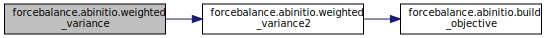
\includegraphics[width=350pt]{namespaceforcebalance_1_1abinitio_aba970cb59bab95eec79027ea05655110_cgraph}
\end{center}
\end{figure}


\hypertarget{namespaceforcebalance_1_1abinitio_ab9554761125a4ec7c3c13d6ae4ea537d}{\index{forcebalance\-::abinitio@{forcebalance\-::abinitio}!weighted\-\_\-variance2@{weighted\-\_\-variance2}}
\index{weighted\-\_\-variance2@{weighted\-\_\-variance2}!forcebalance::abinitio@{forcebalance\-::abinitio}}
\paragraph[{weighted\-\_\-variance2}]{\setlength{\rightskip}{0pt plus 5cm}def {\bf forcebalance.\-abinitio.\-weighted\-\_\-variance2} (
\begin{DoxyParamCaption}
\item[{}]{\-S\-Pi\-Xi, }
\item[{}]{\-W\-Ci\-W, }
\item[{}]{\-Z, }
\item[{}]{\-L, }
\item[{}]{\-R, }
\item[{}]{\-L2, }
\item[{}]{\-R2, }
\item[{}]{\-N\-C\-P1, }
\item[{}]{subtract\-\_\-mean = {\ttfamily \-True}}
\end{DoxyParamCaption}
)}}\label{namespaceforcebalance_1_1abinitio_ab9554761125a4ec7c3c13d6ae4ea537d}


\-A bit of a hack, since we have to subtract out two mean quantities to get \-Hessian elements. 



\-Definition at line 1138 of file abinitio.\-py.



\-Here is the call graph for this function\-:\nopagebreak
\begin{figure}[H]
\begin{center}
\leavevmode
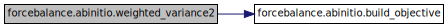
\includegraphics[width=350pt]{namespaceforcebalance_1_1abinitio_ab9554761125a4ec7c3c13d6ae4ea537d_cgraph}
\end{center}
\end{figure}




\subsubsection{\-Variable \-Documentation}
\hypertarget{namespaceforcebalance_1_1abinitio_ae2b6e10e893811325c7103493ac30921}{\index{forcebalance\-::abinitio@{forcebalance\-::abinitio}!logger@{logger}}
\index{logger@{logger}!forcebalance::abinitio@{forcebalance\-::abinitio}}
\paragraph[{logger}]{\setlength{\rightskip}{0pt plus 5cm}tuple {\bf forcebalance\-::abinitio\-::logger} = get\-Logger(\-\_\-\-\_\-name\-\_\-\-\_\-)}}\label{namespaceforcebalance_1_1abinitio_ae2b6e10e893811325c7103493ac30921}


\-Definition at line 24 of file abinitio.\-py.


\hypertarget{namespaceforcebalance_1_1abinitio__internal}{}\subsection{forcebalance.\+abinitio\+\_\+internal Namespace Reference}
\label{namespaceforcebalance_1_1abinitio__internal}\index{forcebalance.\+abinitio\+\_\+internal@{forcebalance.\+abinitio\+\_\+internal}}


Internal implementation of energy matching (for T\+I\+P3P water only)  




\subsubsection{Detailed Description}
Internal implementation of energy matching (for T\+I\+P3P water only) 

\begin{DoxyAuthor}{Author}
Lee-\/\+Ping Wang 
\end{DoxyAuthor}
\begin{DoxyDate}{Date}
04/2012 
\end{DoxyDate}

\hypertarget{namespaceforcebalance_1_1amberio}{\subsection{forcebalance.\-amberio Namespace Reference}
\label{namespaceforcebalance_1_1amberio}\index{forcebalance.\-amberio@{forcebalance.\-amberio}}
}

\hypertarget{namespaceforcebalance_1_1binding}{}\subsection{forcebalance.\+binding Namespace Reference}
\label{namespaceforcebalance_1_1binding}\index{forcebalance.\+binding@{forcebalance.\+binding}}


Binding energy fitting module.  




\subsubsection{Detailed Description}
Binding energy fitting module. 

\begin{DoxyAuthor}{Author}
Lee-\/\+Ping Wang 
\end{DoxyAuthor}
\begin{DoxyDate}{Date}
05/2012 
\end{DoxyDate}

\hypertarget{namespaceforcebalance_1_1chemistry}{\subsection{forcebalance\-:\-:chemistry \-Namespace \-Reference}
\label{namespaceforcebalance_1_1chemistry}\index{forcebalance\-::chemistry@{forcebalance\-::chemistry}}
}
\subsubsection*{\-Functions}
\begin{DoxyCompactItemize}
\item 
def \hyperlink{namespaceforcebalance_1_1chemistry_a7f1904563d4cc7623dcc4fdab5c645a0}{\-Lookup\-By\-Mass}
\item 
def \hyperlink{namespaceforcebalance_1_1chemistry_a843280e0ccfc3059271008be88b38a42}{\-Bond\-Strength\-By\-Length}
\end{DoxyCompactItemize}
\subsubsection*{\-Variables}
\begin{DoxyCompactItemize}
\item 
tuple \hyperlink{namespaceforcebalance_1_1chemistry_aa32672abf21f3992401f7869fef4b579}{\-Bond\-Energies} = defaultdict(lambda\-:defaultdict(dict))
\item 
list \hyperlink{namespaceforcebalance_1_1chemistry_a5db7a023d3980e17137379852d5c8551}{\-Radii}
\begin{DoxyCompactList}\small\item\em \-Covalent radii from \-Cordero et al. \end{DoxyCompactList}\item 
dictionary \hyperlink{namespaceforcebalance_1_1chemistry_a10486086db3bcc2c63c591c726b3464f}{\-Periodic\-Table}
\item 
list \hyperlink{namespaceforcebalance_1_1chemistry_a12ef5f22f5cc3798107d3585c77a1c84}{\-Elements}
\item 
list \hyperlink{namespaceforcebalance_1_1chemistry_a70b1983d2e59ef37617b0a80a3fd14c9}{\-Bond\-Chars} = \mbox{[}'-\/','=','3'\mbox{]}
\item 
string \hyperlink{namespaceforcebalance_1_1chemistry_a244dd58baf4c171b37316e64561c1021}{data\-\_\-from\-\_\-web}
\item 
tuple \hyperlink{namespaceforcebalance_1_1chemistry_a43d08c70d93e430fc6fd6689f622b61b}{line} = line.\-expandtabs()
\item 
tuple \hyperlink{namespaceforcebalance_1_1chemistry_a2e8b0b69254f9a7346919dc00f606e74}{\-B\-E} = float(line.\-split()\mbox{[}1\mbox{]})
\item 
tuple \hyperlink{namespaceforcebalance_1_1chemistry_ace6400fcf0f12a9d9f70aa7496984379}{\-L} = float(line.\-split()\mbox{[}2\mbox{]})
\item 
tuple \hyperlink{namespaceforcebalance_1_1chemistry_a769e0e6c4bad669c6786d1ff12354978}{atoms} = re.\-split('\mbox{[}-\/=3\mbox{]}', line.\-split()\mbox{[}0\mbox{]})
\item 
list \hyperlink{namespaceforcebalance_1_1chemistry_a4f490f29c23b8f185dc926e38eb7e746}{\-A} = \hyperlink{namespaceforcebalance_1_1chemistry_a769e0e6c4bad669c6786d1ff12354978}{atoms}\mbox{[}0\mbox{]}
\item 
list \hyperlink{namespaceforcebalance_1_1chemistry_a408afe99c28b09783c769307b8819f78}{\-B} = \hyperlink{namespaceforcebalance_1_1chemistry_a769e0e6c4bad669c6786d1ff12354978}{atoms}\mbox{[}1\mbox{]}
\item 
tuple \hyperlink{namespaceforcebalance_1_1chemistry_a1ef8f483a40113a668ff3743bb56d7ad}{bo} = \-Bond\-Chars.\-index(re.\-findall('\mbox{[}-\/=3\mbox{]}', line.\-split()\mbox{[}0\mbox{]})\mbox{[}0\mbox{]})
\end{DoxyCompactItemize}


\subsubsection{\-Function \-Documentation}
\hypertarget{namespaceforcebalance_1_1chemistry_a843280e0ccfc3059271008be88b38a42}{\index{forcebalance\-::chemistry@{forcebalance\-::chemistry}!\-Bond\-Strength\-By\-Length@{\-Bond\-Strength\-By\-Length}}
\index{\-Bond\-Strength\-By\-Length@{\-Bond\-Strength\-By\-Length}!forcebalance::chemistry@{forcebalance\-::chemistry}}
\paragraph[{\-Bond\-Strength\-By\-Length}]{\setlength{\rightskip}{0pt plus 5cm}def {\bf forcebalance.\-chemistry.\-Bond\-Strength\-By\-Length} (
\begin{DoxyParamCaption}
\item[{}]{\-A, }
\item[{}]{\-B, }
\item[{}]{length, }
\item[{}]{artol = {\ttfamily 0.33}, }
\item[{}]{bias = {\ttfamily 0.0}}
\end{DoxyParamCaption}
)}}\label{namespaceforcebalance_1_1chemistry_a843280e0ccfc3059271008be88b38a42}


\-Definition at line 164 of file chemistry.\-py.

\hypertarget{namespaceforcebalance_1_1chemistry_a7f1904563d4cc7623dcc4fdab5c645a0}{\index{forcebalance\-::chemistry@{forcebalance\-::chemistry}!\-Lookup\-By\-Mass@{\-Lookup\-By\-Mass}}
\index{\-Lookup\-By\-Mass@{\-Lookup\-By\-Mass}!forcebalance::chemistry@{forcebalance\-::chemistry}}
\paragraph[{\-Lookup\-By\-Mass}]{\setlength{\rightskip}{0pt plus 5cm}def {\bf forcebalance.\-chemistry.\-Lookup\-By\-Mass} (
\begin{DoxyParamCaption}
\item[{}]{mass}
\end{DoxyParamCaption}
)}}\label{namespaceforcebalance_1_1chemistry_a7f1904563d4cc7623dcc4fdab5c645a0}


\-Definition at line 155 of file chemistry.\-py.



\subsubsection{\-Variable \-Documentation}
\hypertarget{namespaceforcebalance_1_1chemistry_a4f490f29c23b8f185dc926e38eb7e746}{\index{forcebalance\-::chemistry@{forcebalance\-::chemistry}!\-A@{\-A}}
\index{\-A@{\-A}!forcebalance::chemistry@{forcebalance\-::chemistry}}
\paragraph[{\-A}]{\setlength{\rightskip}{0pt plus 5cm}list {\bf forcebalance\-::chemistry\-::\-A} = {\bf atoms}\mbox{[}0\mbox{]}}}\label{namespaceforcebalance_1_1chemistry_a4f490f29c23b8f185dc926e38eb7e746}


\-Definition at line 149 of file chemistry.\-py.

\hypertarget{namespaceforcebalance_1_1chemistry_a769e0e6c4bad669c6786d1ff12354978}{\index{forcebalance\-::chemistry@{forcebalance\-::chemistry}!atoms@{atoms}}
\index{atoms@{atoms}!forcebalance::chemistry@{forcebalance\-::chemistry}}
\paragraph[{atoms}]{\setlength{\rightskip}{0pt plus 5cm}tuple {\bf forcebalance\-::chemistry\-::atoms} = re.\-split('\mbox{[}-\/=3\mbox{]}', line.\-split()\mbox{[}0\mbox{]})}}\label{namespaceforcebalance_1_1chemistry_a769e0e6c4bad669c6786d1ff12354978}


\-Definition at line 148 of file chemistry.\-py.

\hypertarget{namespaceforcebalance_1_1chemistry_a408afe99c28b09783c769307b8819f78}{\index{forcebalance\-::chemistry@{forcebalance\-::chemistry}!\-B@{\-B}}
\index{\-B@{\-B}!forcebalance::chemistry@{forcebalance\-::chemistry}}
\paragraph[{\-B}]{\setlength{\rightskip}{0pt plus 5cm}list {\bf forcebalance\-::chemistry\-::\-B} = {\bf atoms}\mbox{[}1\mbox{]}}}\label{namespaceforcebalance_1_1chemistry_a408afe99c28b09783c769307b8819f78}


\-Definition at line 150 of file chemistry.\-py.

\hypertarget{namespaceforcebalance_1_1chemistry_a2e8b0b69254f9a7346919dc00f606e74}{\index{forcebalance\-::chemistry@{forcebalance\-::chemistry}!\-B\-E@{\-B\-E}}
\index{\-B\-E@{\-B\-E}!forcebalance::chemistry@{forcebalance\-::chemistry}}
\paragraph[{\-B\-E}]{\setlength{\rightskip}{0pt plus 5cm}tuple {\bf forcebalance\-::chemistry\-::\-B\-E} = float(line.\-split()\mbox{[}1\mbox{]})}}\label{namespaceforcebalance_1_1chemistry_a2e8b0b69254f9a7346919dc00f606e74}


\-Definition at line 146 of file chemistry.\-py.

\hypertarget{namespaceforcebalance_1_1chemistry_a1ef8f483a40113a668ff3743bb56d7ad}{\index{forcebalance\-::chemistry@{forcebalance\-::chemistry}!bo@{bo}}
\index{bo@{bo}!forcebalance::chemistry@{forcebalance\-::chemistry}}
\paragraph[{bo}]{\setlength{\rightskip}{0pt plus 5cm}tuple {\bf forcebalance\-::chemistry\-::bo} = \-Bond\-Chars.\-index(re.\-findall('\mbox{[}-\/=3\mbox{]}', line.\-split()\mbox{[}0\mbox{]})\mbox{[}0\mbox{]})}}\label{namespaceforcebalance_1_1chemistry_a1ef8f483a40113a668ff3743bb56d7ad}


\-Definition at line 151 of file chemistry.\-py.

\hypertarget{namespaceforcebalance_1_1chemistry_a70b1983d2e59ef37617b0a80a3fd14c9}{\index{forcebalance\-::chemistry@{forcebalance\-::chemistry}!\-Bond\-Chars@{\-Bond\-Chars}}
\index{\-Bond\-Chars@{\-Bond\-Chars}!forcebalance::chemistry@{forcebalance\-::chemistry}}
\paragraph[{\-Bond\-Chars}]{\setlength{\rightskip}{0pt plus 5cm}list {\bf forcebalance\-::chemistry\-::\-Bond\-Chars} = \mbox{[}'-\/','=','3'\mbox{]}}}\label{namespaceforcebalance_1_1chemistry_a70b1983d2e59ef37617b0a80a3fd14c9}


\-Definition at line 49 of file chemistry.\-py.

\hypertarget{namespaceforcebalance_1_1chemistry_aa32672abf21f3992401f7869fef4b579}{\index{forcebalance\-::chemistry@{forcebalance\-::chemistry}!\-Bond\-Energies@{\-Bond\-Energies}}
\index{\-Bond\-Energies@{\-Bond\-Energies}!forcebalance::chemistry@{forcebalance\-::chemistry}}
\paragraph[{\-Bond\-Energies}]{\setlength{\rightskip}{0pt plus 5cm}tuple {\bf forcebalance\-::chemistry\-::\-Bond\-Energies} = defaultdict(lambda\-:defaultdict(dict))}}\label{namespaceforcebalance_1_1chemistry_aa32672abf21f3992401f7869fef4b579}


\-Definition at line 7 of file chemistry.\-py.

\hypertarget{namespaceforcebalance_1_1chemistry_a244dd58baf4c171b37316e64561c1021}{\index{forcebalance\-::chemistry@{forcebalance\-::chemistry}!data\-\_\-from\-\_\-web@{data\-\_\-from\-\_\-web}}
\index{data\-\_\-from\-\_\-web@{data\-\_\-from\-\_\-web}!forcebalance::chemistry@{forcebalance\-::chemistry}}
\paragraph[{data\-\_\-from\-\_\-web}]{\setlength{\rightskip}{0pt plus 5cm}string {\bf forcebalance\-::chemistry\-::data\-\_\-from\-\_\-web}}}\label{namespaceforcebalance_1_1chemistry_a244dd58baf4c171b37316e64561c1021}


\-Definition at line 51 of file chemistry.\-py.

\hypertarget{namespaceforcebalance_1_1chemistry_a12ef5f22f5cc3798107d3585c77a1c84}{\index{forcebalance\-::chemistry@{forcebalance\-::chemistry}!\-Elements@{\-Elements}}
\index{\-Elements@{\-Elements}!forcebalance::chemistry@{forcebalance\-::chemistry}}
\paragraph[{\-Elements}]{\setlength{\rightskip}{0pt plus 5cm}list {\bf forcebalance\-::chemistry\-::\-Elements}}}\label{namespaceforcebalance_1_1chemistry_a12ef5f22f5cc3798107d3585c77a1c84}
{\bfseries \-Initial value\-:}
\begin{DoxyCode}
1 ["None",'H','He',
2             'Li','Be','B','C','N','O','F','Ne',
3             'Na','Mg','Al','Si','P','S','Cl','Ar',
4             'K','Ca','Sc','Ti','V','Cr','Mn','Fe','Co','Ni','Cu','Zn','Ga','Ge'
      ,'As','Se','Br','Kr',
5             'Rb','Sr','Y','Zr','Nb','Mo','Tc','Ru','Rh','Pd','Ag','Cd','In','Sn
      ','Sb','Te','I','Xe',
6             'Cs','Ba','La','Ce','Pr','Nd','Pm','Sm','Eu','Gd','Tb','Dy','Ho','
      Er','Tm','Yb',
7             'Lu','Hf','Ta','W','Re','Os','Ir','Pt','Au','Hg','Tl','Pb','Bi','Po
      ','At','Rn',
8             'Fr','Ra','Ac','Th','Pa','U','Np','Pu','Am','Cm','Bk','Cf','Es','Fm
      ','Md','No','Lr','Rf','Db','Sg','Bh','Hs','Mt']
\end{DoxyCode}


\-Definition at line 40 of file chemistry.\-py.

\hypertarget{namespaceforcebalance_1_1chemistry_ace6400fcf0f12a9d9f70aa7496984379}{\index{forcebalance\-::chemistry@{forcebalance\-::chemistry}!\-L@{\-L}}
\index{\-L@{\-L}!forcebalance::chemistry@{forcebalance\-::chemistry}}
\paragraph[{\-L}]{\setlength{\rightskip}{0pt plus 5cm}tuple {\bf forcebalance\-::chemistry\-::\-L} = float(line.\-split()\mbox{[}2\mbox{]})}}\label{namespaceforcebalance_1_1chemistry_ace6400fcf0f12a9d9f70aa7496984379}


\-Definition at line 147 of file chemistry.\-py.

\hypertarget{namespaceforcebalance_1_1chemistry_a43d08c70d93e430fc6fd6689f622b61b}{\index{forcebalance\-::chemistry@{forcebalance\-::chemistry}!line@{line}}
\index{line@{line}!forcebalance::chemistry@{forcebalance\-::chemistry}}
\paragraph[{line}]{\setlength{\rightskip}{0pt plus 5cm}tuple {\bf forcebalance\-::chemistry\-::line} = line.\-expandtabs()}}\label{namespaceforcebalance_1_1chemistry_a43d08c70d93e430fc6fd6689f622b61b}


\-Definition at line 145 of file chemistry.\-py.

\hypertarget{namespaceforcebalance_1_1chemistry_a10486086db3bcc2c63c591c726b3464f}{\index{forcebalance\-::chemistry@{forcebalance\-::chemistry}!\-Periodic\-Table@{\-Periodic\-Table}}
\index{\-Periodic\-Table@{\-Periodic\-Table}!forcebalance::chemistry@{forcebalance\-::chemistry}}
\paragraph[{\-Periodic\-Table}]{\setlength{\rightskip}{0pt plus 5cm}dictionary {\bf forcebalance\-::chemistry\-::\-Periodic\-Table}}}\label{namespaceforcebalance_1_1chemistry_a10486086db3bcc2c63c591c726b3464f}
{\bfseries \-Initial value\-:}
\begin{DoxyCode}
1 {'H' : 1.0079, 'He' : 4.0026, 
2                  'Li' : 6.941, 'Be' : 9.0122, 'B' : 10.811, 'C' : 12.0107, 'N' 
      : 14.0067, 'O' : 15.9994, 'F' : 18.9984, 'Ne' : 20.1797,
3                  'Na' : 22.9897, 'Mg' : 24.305, 'Al' : 26.9815, 'Si' : 28.0855,
       'P' : 30.9738, 'S' : 32.065, 'Cl' : 35.453, 'Ar' : 39.948, 
4                  'K' : 39.0983, 'Ca' : 40.078, 'Sc' : 44.9559, 'Ti' : 47.867, '
      V' : 50.9415, 'Cr' : 51.9961, 'Mn' : 54.938, 'Fe' : 55.845, 'Co' : 58.9332, 
5                  'Ni' : 58.6934, 'Cu' : 63.546, 'Zn' : 65.39, 'Ga' : 69.723, '
      Ge' : 72.64, 'As' : 74.9216, 'Se' : 78.96, 'Br' : 79.904, 'Kr' : 83.8, 
6                  'Rb' : 85.4678, 'Sr' : 87.62, 'Y' : 88.9059, 'Zr' : 91.224, '
      Nb' : 92.9064, 'Mo' : 95.94, 'Tc' : 98, 'Ru' : 101.07, 'Rh' : 102.9055, 
7                  'Pd' : 106.42, 'Ag' : 107.8682, 'Cd' : 112.411, 'In' : 114.818
      , 'Sn' : 118.71, 'Sb' : 121.76, 'Te' : 127.6, 'I' : 126.9045, 'Xe' : 131.293, 
8                  'Cs' : 132.9055, 'Ba' : 137.327, 'La' : 138.9055, 'Ce' : 140.1
      16, 'Pr' : 140.9077, 'Nd' : 144.24, 'Pm' : 145, 'Sm' : 150.36, 
9                  'Eu' : 151.964, 'Gd' : 157.25, 'Tb' : 158.9253, 'Dy' : 162.5, 
      'Ho' : 164.9303, 'Er' : 167.259, 'Tm' : 168.9342, 'Yb' : 173.04, 
10                  'Lu' : 174.967, 'Hf' : 178.49, 'Ta' : 180.9479, 'W' : 183.84, 
      'Re' : 186.207, 'Os' : 190.23, 'Ir' : 192.217, 'Pt' : 195.078, 
11                  'Au' : 196.9665, 'Hg' : 200.59, 'Tl' : 204.3833, 'Pb' : 207.2,
       'Bi' : 208.9804, 'Po' : 209, 'At' : 210, 'Rn' : 222, 
12                  'Fr' : 223, 'Ra' : 226, 'Ac' : 227, 'Th' : 232.0381, 'Pa' : 23
      1.0359, 'U' : 238.0289, 'Np' : 237, 'Pu' : 244, 
13                  'Am' : 243, 'Cm' : 247, 'Bk' : 247, 'Cf' : 251, 'Es' : 252, '
      Fm' : 257, 'Md' : 258, 'No' : 259, 
14                  'Lr' : 262, 'Rf' : 261, 'Db' : 262, 'Sg' : 266, 'Bh' : 264, '
      Hs' : 277, 'Mt' : 268}
\end{DoxyCode}


\-Definition at line 25 of file chemistry.\-py.

\hypertarget{namespaceforcebalance_1_1chemistry_a5db7a023d3980e17137379852d5c8551}{\index{forcebalance\-::chemistry@{forcebalance\-::chemistry}!\-Radii@{\-Radii}}
\index{\-Radii@{\-Radii}!forcebalance::chemistry@{forcebalance\-::chemistry}}
\paragraph[{\-Radii}]{\setlength{\rightskip}{0pt plus 5cm}list {\bf forcebalance\-::chemistry\-::\-Radii}}}\label{namespaceforcebalance_1_1chemistry_a5db7a023d3980e17137379852d5c8551}
{\bfseries \-Initial value\-:}
\begin{DoxyCode}
1 [0.31, 0.28, # H and He
2          1.28, 0.96, 0.84, 0.76, 0.71, 0.66, 0.57, 0.58, # First row elements
3          1.66, 1.41, 1.21, 1.11, 1.07, 1.05, 1.02, 1.06, # Second row elements
4          2.03, 1.76, 1.70, 1.60, 1.53, 1.39, 1.61, 1.52, 1.50, 
5          1.24, 1.32, 1.22, 1.22, 1.20, 1.19, 1.20, 1.20, 1.16, # Third row
       elements, K through Kr
6          2.20, 1.95, 1.90, 1.75, 1.64, 1.54, 1.47, 1.46, 1.42, 
7          1.39, 1.45, 1.44, 1.42, 1.39, 1.39, 1.38, 1.39, 1.40, # Fourth row
       elements, Rb through Xe
8          2.44, 2.15, 2.07, 2.04, 2.03, 2.01, 1.99, 1.98, 
9          1.98, 1.96, 1.94, 1.92, 1.92, 1.89, 1.90, 1.87, # Fifth row elements,
       s and f blocks
10          1.87, 1.75, 1.70, 1.62, 1.51, 1.44, 1.41, 1.36, 
11          1.36, 1.32, 1.45, 1.46, 1.48, 1.40, 1.50, 1.50, # Fifth row elements,
       d and p blocks
12          2.60, 2.21, 2.15, 2.06, 2.00, 1.96, 1.90, 1.87, 1.80, 1.69]
\end{DoxyCode}


\-Covalent radii from \-Cordero et al. 

'\-Covalent radii revisited' \-Dalton \-Transactions 2008, 2832-\/2838. 

\-Definition at line 10 of file chemistry.\-py.


\hypertarget{namespaceforcebalance_1_1contact}{\subsection{forcebalance.\-contact Namespace Reference}
\label{namespaceforcebalance_1_1contact}\index{forcebalance.\-contact@{forcebalance.\-contact}}
}
\subsubsection*{Functions}
\begin{DoxyCompactItemize}
\item 
def \hyperlink{namespaceforcebalance_1_1contact_a3592dbbf524c6115f34d9a70b50e2e0f}{atom\-\_\-distances}
\begin{DoxyCompactList}\small\item\em For each frame in xyzlist, compute the (euclidean) distance between pairs of atoms whos indices are given in contacts. \end{DoxyCompactList}\item 
def \hyperlink{namespaceforcebalance_1_1contact_acffb04a66580454b8a87648faa1c5c16}{residue\-\_\-distances}
\begin{DoxyCompactList}\small\item\em For each frame in xyzlist, and for each pair of residues in the array contact, compute the distance between the closest pair of atoms such that one of them belongs to each residue. \end{DoxyCompactList}\end{DoxyCompactItemize}


\subsubsection{Function Documentation}
\hypertarget{namespaceforcebalance_1_1contact_a3592dbbf524c6115f34d9a70b50e2e0f}{\index{forcebalance\-::contact@{forcebalance\-::contact}!atom\-\_\-distances@{atom\-\_\-distances}}
\index{atom\-\_\-distances@{atom\-\_\-distances}!forcebalance::contact@{forcebalance\-::contact}}
\paragraph[{atom\-\_\-distances}]{\setlength{\rightskip}{0pt plus 5cm}def forcebalance.\-contact.\-atom\-\_\-distances (
\begin{DoxyParamCaption}
\item[{}]{xyzlist, }
\item[{}]{atom\-\_\-contacts}
\end{DoxyParamCaption}
)}}\label{namespaceforcebalance_1_1contact_a3592dbbf524c6115f34d9a70b50e2e0f}


For each frame in xyzlist, compute the (euclidean) distance between pairs of atoms whos indices are given in contacts. 

xyzlist should be a traj\-\_\-length x num\-\_\-atoms x num\-\_\-dims array of type float32

contacts should be a num\-\_\-contacts x 2 array where each row gives the indices of 2 atoms whos distance you care to monitor.

Returns\-: traj\-\_\-length x num\-\_\-contacts array of euclidean distances

Note\-: For nice wrappers around this, see the prepare\-\_\-trajectory method of various metrics in metrics.\-py 

Definition at line 26 of file contact.\-py.



Here is the call graph for this function\-:
\nopagebreak
\begin{figure}[H]
\begin{center}
\leavevmode
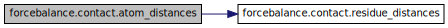
\includegraphics[width=350pt]{namespaceforcebalance_1_1contact_a3592dbbf524c6115f34d9a70b50e2e0f_cgraph}
\end{center}
\end{figure}


\hypertarget{namespaceforcebalance_1_1contact_acffb04a66580454b8a87648faa1c5c16}{\index{forcebalance\-::contact@{forcebalance\-::contact}!residue\-\_\-distances@{residue\-\_\-distances}}
\index{residue\-\_\-distances@{residue\-\_\-distances}!forcebalance::contact@{forcebalance\-::contact}}
\paragraph[{residue\-\_\-distances}]{\setlength{\rightskip}{0pt plus 5cm}def forcebalance.\-contact.\-residue\-\_\-distances (
\begin{DoxyParamCaption}
\item[{}]{xyzlist, }
\item[{}]{residue\-\_\-membership, }
\item[{}]{residue\-\_\-contacts}
\end{DoxyParamCaption}
)}}\label{namespaceforcebalance_1_1contact_acffb04a66580454b8a87648faa1c5c16}


For each frame in xyzlist, and for each pair of residues in the array contact, compute the distance between the closest pair of atoms such that one of them belongs to each residue. 

xyzlist should be a traj\-\_\-length x num\-\_\-atoms x num\-\_\-dims array of type float32

residue\-\_\-membership should be a list of lists where residue\-\_\-membership\mbox{[}i\mbox{]} gives the list of atomindices that belong to residue i. residue\-\_\-membership should N\-O\-T be a numpy 2\-D array unless you really mean that all of the residues have the same number of atoms

residue\-\_\-contacts should be a 2\-D numpy array of shape num\-\_\-contacts x 2 where each row gives the indices of the two R\-E\-S\-I\-D\-U\-E\-S who you are interested in monitoring for a contact.

Returns\-: a 2\-D array of traj\-\_\-lenth x num\-\_\-contacts where out\mbox{[}i,j\mbox{]} contains the distance between the pair of atoms, one from residue\-\_\-membership\mbox{[}residue\-\_\-contacts\mbox{[}j,0\mbox{]}\mbox{]} and one from residue\-\_\-membership\mbox{[}residue\-\_\-contacts\mbox{[}j,1\mbox{]}\mbox{]} that are closest. 

Definition at line 85 of file contact.\-py.


\hypertarget{namespaceforcebalance_1_1counterpoise}{\subsection{forcebalance.\-counterpoise Namespace Reference}
\label{namespaceforcebalance_1_1counterpoise}\index{forcebalance.\-counterpoise@{forcebalance.\-counterpoise}}
}


Match an empirical potential to the counterpoise correction for basis set superposition error (B\-S\-S\-E).  


\subsubsection*{Classes}
\begin{DoxyCompactItemize}
\item 
class \hyperlink{classforcebalance_1_1counterpoise_1_1Counterpoise}{Counterpoise}
\begin{DoxyCompactList}\small\item\em Target subclass for matching the counterpoise correction. \end{DoxyCompactList}\end{DoxyCompactItemize}


\subsubsection{Detailed Description}
Match an empirical potential to the counterpoise correction for basis set superposition error (B\-S\-S\-E). Here we test two different functional forms\-: a three-\/parameter Gaussian repulsive potential and a four-\/parameter Gaussian which goes smoothly to an exponential. The latter can be written in two different ways -\/ one which gives us control over the exponential, the switching distance and the Gaussian decay constant, and another which gives us control over the Gaussian and the switching distance. They are called 'C\-P\-G\-A\-U\-S\-S', 'C\-P\-E\-X\-P\-G', and 'C\-P\-G\-E\-X\-P'. I think the third option is the best although our early tests have indicated that none of the force fields perform particularly well for the water dimer.

This subclass of Target implements the 'get' method.

\begin{DoxyAuthor}{Author}
Lee-\/\-Ping Wang 
\end{DoxyAuthor}
\begin{DoxyDate}{Date}
12/2011 
\end{DoxyDate}

\hypertarget{namespaceforcebalance_1_1custom__io}{\subsection{forcebalance\-:\-:custom\-\_\-io \-Namespace \-Reference}
\label{namespaceforcebalance_1_1custom__io}\index{forcebalance\-::custom\-\_\-io@{forcebalance\-::custom\-\_\-io}}
}


\-Custom force field parser.  


\subsubsection*{\-Classes}
\begin{DoxyCompactItemize}
\item 
class \hyperlink{classforcebalance_1_1custom__io_1_1Gen__Reader}{\-Gen\-\_\-\-Reader}
\begin{DoxyCompactList}\small\item\em \-Finite state machine for parsing custom \-G\-R\-O\-M\-A\-C\-S force field files. \end{DoxyCompactList}\end{DoxyCompactItemize}
\subsubsection*{\-Variables}
\begin{DoxyCompactItemize}
\item 
list \hyperlink{namespaceforcebalance_1_1custom__io_a509d4c2b5eeee4278adde414e55eb560}{cptypes} = \mbox{[}\-None, '\-C\-P\-G\-A\-U\-S\-S', '\-C\-P\-E\-X\-P\-G', '\-C\-P\-G\-E\-X\-P'\mbox{]}
\begin{DoxyCompactList}\small\item\em \-Types of counterpoise correction. \end{DoxyCompactList}\item 
list \hyperlink{namespaceforcebalance_1_1custom__io_a604fd5cd1f0c6057a8a72ac61b55f6fa}{ndtypes} = \mbox{[}\-None\mbox{]}
\begin{DoxyCompactList}\small\item\em \-Types of \-N\-D\-D\-O correction. \end{DoxyCompactList}\item 
dictionary \hyperlink{namespaceforcebalance_1_1custom__io_a64c7f292c64ad2b2b855a82e68c0ca7e}{fdict}
\begin{DoxyCompactList}\small\item\em \-Section -\/$>$ \-Interaction type dictionary. \end{DoxyCompactList}\item 
dictionary \hyperlink{namespaceforcebalance_1_1custom__io_aaa87b8099dee5dfec42f5869dabad0c5}{pdict}
\begin{DoxyCompactList}\small\item\em \-Interaction type -\/$>$ \-Parameter \-Dictionary. \end{DoxyCompactList}\end{DoxyCompactItemize}


\subsubsection{\-Detailed \-Description}
\-Custom force field parser. \-We take advantage of the sections in \-G\-R\-O\-M\-A\-C\-S and the 'interaction type' concept, but these interactions are not supported in \-G\-R\-O\-M\-A\-C\-S; rather, they are computed within our program.

\begin{DoxyAuthor}{\-Author}
\-Lee-\/\-Ping \-Wang 
\end{DoxyAuthor}
\begin{DoxyDate}{\-Date}
12/2011 
\end{DoxyDate}


\subsubsection{\-Variable \-Documentation}
\hypertarget{namespaceforcebalance_1_1custom__io_a509d4c2b5eeee4278adde414e55eb560}{\index{forcebalance\-::custom\-\_\-io@{forcebalance\-::custom\-\_\-io}!cptypes@{cptypes}}
\index{cptypes@{cptypes}!forcebalance::custom_io@{forcebalance\-::custom\-\_\-io}}
\paragraph[{cptypes}]{\setlength{\rightskip}{0pt plus 5cm}list {\bf forcebalance\-::custom\-\_\-io\-::cptypes} = \mbox{[}\-None, '\-C\-P\-G\-A\-U\-S\-S', '\-C\-P\-E\-X\-P\-G', '\-C\-P\-G\-E\-X\-P'\mbox{]}}}\label{namespaceforcebalance_1_1custom__io_a509d4c2b5eeee4278adde414e55eb560}


\-Types of counterpoise correction. 



\-Definition at line 16 of file custom\-\_\-io.\-py.

\hypertarget{namespaceforcebalance_1_1custom__io_a64c7f292c64ad2b2b855a82e68c0ca7e}{\index{forcebalance\-::custom\-\_\-io@{forcebalance\-::custom\-\_\-io}!fdict@{fdict}}
\index{fdict@{fdict}!forcebalance::custom_io@{forcebalance\-::custom\-\_\-io}}
\paragraph[{fdict}]{\setlength{\rightskip}{0pt plus 5cm}dictionary {\bf forcebalance\-::custom\-\_\-io\-::fdict}}}\label{namespaceforcebalance_1_1custom__io_a64c7f292c64ad2b2b855a82e68c0ca7e}
{\bfseries \-Initial value\-:}
\begin{DoxyCode}
1 {
2     'counterpoise'  : cptypes    }
\end{DoxyCode}


\-Section -\/$>$ \-Interaction type dictionary. 



\-Definition at line 21 of file custom\-\_\-io.\-py.

\hypertarget{namespaceforcebalance_1_1custom__io_a604fd5cd1f0c6057a8a72ac61b55f6fa}{\index{forcebalance\-::custom\-\_\-io@{forcebalance\-::custom\-\_\-io}!ndtypes@{ndtypes}}
\index{ndtypes@{ndtypes}!forcebalance::custom_io@{forcebalance\-::custom\-\_\-io}}
\paragraph[{ndtypes}]{\setlength{\rightskip}{0pt plus 5cm}list {\bf forcebalance\-::custom\-\_\-io\-::ndtypes} = \mbox{[}\-None\mbox{]}}}\label{namespaceforcebalance_1_1custom__io_a604fd5cd1f0c6057a8a72ac61b55f6fa}


\-Types of \-N\-D\-D\-O correction. 



\-Definition at line 18 of file custom\-\_\-io.\-py.

\hypertarget{namespaceforcebalance_1_1custom__io_aaa87b8099dee5dfec42f5869dabad0c5}{\index{forcebalance\-::custom\-\_\-io@{forcebalance\-::custom\-\_\-io}!pdict@{pdict}}
\index{pdict@{pdict}!forcebalance::custom_io@{forcebalance\-::custom\-\_\-io}}
\paragraph[{pdict}]{\setlength{\rightskip}{0pt plus 5cm}dictionary {\bf forcebalance\-::custom\-\_\-io\-::pdict}}}\label{namespaceforcebalance_1_1custom__io_aaa87b8099dee5dfec42f5869dabad0c5}
{\bfseries \-Initial value\-:}
\begin{DoxyCode}
1 {'CPGAUSS':{3:'A', 4:'B', 5:'C'},
2          'CPGEXP' :{3:'A', 4:'B', 5:'G', 6:'X'},
3          'CPEXPG' :{3:'A1', 4:'B', 5:'X0', 6:'A2'}
4          }
\end{DoxyCode}


\-Interaction type -\/$>$ \-Parameter \-Dictionary. 



\-Definition at line 25 of file custom\-\_\-io.\-py.


\hypertarget{namespaceforcebalance_1_1engine}{\subsection{forcebalance.\-engine Namespace Reference}
\label{namespaceforcebalance_1_1engine}\index{forcebalance.\-engine@{forcebalance.\-engine}}
}

\hypertarget{namespaceforcebalance_1_1finite__difference}{\subsection{forcebalance.\-finite\-\_\-difference Namespace Reference}
\label{namespaceforcebalance_1_1finite__difference}\index{forcebalance.\-finite\-\_\-difference@{forcebalance.\-finite\-\_\-difference}}
}

\hypertarget{namespaceforcebalance_1_1forcefield}{\subsection{forcebalance.\-forcefield Namespace Reference}
\label{namespaceforcebalance_1_1forcefield}\index{forcebalance.\-forcefield@{forcebalance.\-forcefield}}
}

\hypertarget{namespaceforcebalance_1_1gmxio}{\subsection{forcebalance.\-gmxio Namespace Reference}
\label{namespaceforcebalance_1_1gmxio}\index{forcebalance.\-gmxio@{forcebalance.\-gmxio}}
}


G\-R\-O\-M\-A\-C\-S input/output.  


\subsubsection*{Classes}
\begin{DoxyCompactItemize}
\item 
class \hyperlink{classforcebalance_1_1gmxio_1_1ITP__Reader}{I\-T\-P\-\_\-\-Reader}
\begin{DoxyCompactList}\small\item\em Finite state machine for parsing G\-R\-O\-M\-A\-C\-S force field files. \end{DoxyCompactList}\item 
class \hyperlink{classforcebalance_1_1gmxio_1_1GMX}{G\-M\-X}
\begin{DoxyCompactList}\small\item\em Derived from Engine object for carrying out general purpose G\-R\-O\-M\-A\-C\-S calculations. \end{DoxyCompactList}\item 
class \hyperlink{classforcebalance_1_1gmxio_1_1AbInitio__GMX}{Ab\-Initio\-\_\-\-G\-M\-X}
\begin{DoxyCompactList}\small\item\em Subclass of Ab\-Initio for force and energy matching using normal G\-R\-O\-M\-A\-C\-S. \end{DoxyCompactList}\item 
class \hyperlink{classforcebalance_1_1gmxio_1_1Liquid__GMX}{Liquid\-\_\-\-G\-M\-X}
\item 
class \hyperlink{classforcebalance_1_1gmxio_1_1Interaction__GMX}{Interaction\-\_\-\-G\-M\-X}
\begin{DoxyCompactList}\small\item\em Subclass of Interaction for interaction energy matching using G\-R\-O\-M\-A\-C\-S. \end{DoxyCompactList}\end{DoxyCompactItemize}
\subsubsection*{Functions}
\begin{DoxyCompactItemize}
\item 
def \hyperlink{namespaceforcebalance_1_1gmxio_acc5bef2c5c991cd70a948a1dd43ef6a6}{edit\-\_\-mdp}
\begin{DoxyCompactList}\small\item\em Create or edit a Gromacs M\-D\-P file. \end{DoxyCompactList}\item 
def \hyperlink{namespaceforcebalance_1_1gmxio_a29af6ace00d7e58258e0a854ca13d954}{parse\-\_\-atomtype\-\_\-line}
\begin{DoxyCompactList}\small\item\em Parses the 'atomtype' line. \end{DoxyCompactList}\item 
def \hyperlink{namespaceforcebalance_1_1gmxio_acac8488f29b62fb0d4cb54bb5a041026}{rm\-\_\-gmx\-\_\-baks}
\end{DoxyCompactItemize}
\subsubsection*{Variables}
\begin{DoxyCompactItemize}
\item 
tuple \hyperlink{namespaceforcebalance_1_1gmxio_ac10457054444ca04e0a265665afc2512}{logger} = get\-Logger(\-\_\-\-\_\-name\-\_\-\-\_\-)
\item 
list \hyperlink{namespaceforcebalance_1_1gmxio_a337bc61280b58a43319380dec9c5529a}{nftypes} = \mbox{[}None, 'V\-D\-W', 'V\-D\-W\-\_\-\-B\-H\-A\-M'\mbox{]}
\begin{DoxyCompactList}\small\item\em Vd\-W interaction function types. \end{DoxyCompactList}\item 
list \hyperlink{namespaceforcebalance_1_1gmxio_a59695b79df36efbe64ac88fd64bfb366}{pftypes} = \mbox{[}None, 'V\-P\-A\-I\-R', 'V\-P\-A\-I\-R\-\_\-\-B\-H\-A\-M'\mbox{]}
\begin{DoxyCompactList}\small\item\em Pairwise interaction function types. \end{DoxyCompactList}\item 
list \hyperlink{namespaceforcebalance_1_1gmxio_a49a34b85d405c9286ceec1e6f088069f}{bftypes} = \mbox{[}None, 'B\-O\-N\-D\-S', 'G96\-B\-O\-N\-D\-S', 'M\-O\-R\-S\-E'\mbox{]}
\begin{DoxyCompactList}\small\item\em Bonded interaction function types. \end{DoxyCompactList}\item 
list \hyperlink{namespaceforcebalance_1_1gmxio_aef89ff391902f81feb14e28ec301296c}{aftypes}
\begin{DoxyCompactList}\small\item\em Angle interaction function types. \end{DoxyCompactList}\item 
list \hyperlink{namespaceforcebalance_1_1gmxio_acd9fed3887161c6386506563fd4f3534}{dftypes} = \mbox{[}None, 'P\-D\-I\-H\-S', 'I\-D\-I\-H\-S', 'R\-B\-D\-I\-H\-S', 'P\-I\-M\-P\-D\-I\-H\-S', 'F\-O\-U\-R\-D\-I\-H\-S', None, None, 'T\-A\-B\-D\-I\-H\-S', 'P\-D\-I\-H\-M\-U\-L\-S'\mbox{]}
\begin{DoxyCompactList}\small\item\em Dihedral interaction function types. \end{DoxyCompactList}\item 
dictionary \hyperlink{namespaceforcebalance_1_1gmxio_a179cbde2e55b4c025af89b225612d6e1}{fdict}
\begin{DoxyCompactList}\small\item\em Section -\/$>$ Interaction type dictionary. \end{DoxyCompactList}\item 
dictionary \hyperlink{namespaceforcebalance_1_1gmxio_ae845e0b923ecde16c79f2742b94534a6}{pdict}
\begin{DoxyCompactList}\small\item\em Interaction type -\/$>$ Parameter Dictionary. \end{DoxyCompactList}\item 
string \hyperlink{namespaceforcebalance_1_1gmxio_a35d747dea4a5446d049d901e782feaa2}{shot\-\_\-mdp}
\end{DoxyCompactItemize}


\subsubsection{Detailed Description}
G\-R\-O\-M\-A\-C\-S input/output. \begin{DoxyRefDesc}{Todo}
\item[\hyperlink{todo__todo000009}{Todo}]Even more stuff from \hyperlink{forcefield_8py}{forcefield.\-py} needs to go into here.\end{DoxyRefDesc}


\begin{DoxyAuthor}{Author}
Lee-\/\-Ping Wang 
\end{DoxyAuthor}
\begin{DoxyDate}{Date}
12/2011
\end{DoxyDate}
\begin{DoxyRefDesc}{Todo}
\item[\hyperlink{todo__todo000012}{Todo}]Even more stuff from \hyperlink{forcefield_8py}{forcefield.\-py} needs to go into here.\end{DoxyRefDesc}


\begin{DoxyAuthor}{Author}
Lee-\/\-Ping Wang 
\end{DoxyAuthor}
\begin{DoxyDate}{Date}
12/2011 
\end{DoxyDate}


\subsubsection{Function Documentation}
\hypertarget{namespaceforcebalance_1_1gmxio_acc5bef2c5c991cd70a948a1dd43ef6a6}{\index{forcebalance\-::gmxio@{forcebalance\-::gmxio}!edit\-\_\-mdp@{edit\-\_\-mdp}}
\index{edit\-\_\-mdp@{edit\-\_\-mdp}!forcebalance::gmxio@{forcebalance\-::gmxio}}
\paragraph[{edit\-\_\-mdp}]{\setlength{\rightskip}{0pt plus 5cm}def forcebalance.\-gmxio.\-edit\-\_\-mdp (
\begin{DoxyParamCaption}
\item[{}]{fin, }
\item[{}]{fout, }
\item[{}]{options, }
\item[{}]{verbose = {\ttfamily False}}
\end{DoxyParamCaption}
)}}\label{namespaceforcebalance_1_1gmxio_acc5bef2c5c991cd70a948a1dd43ef6a6}


Create or edit a Gromacs M\-D\-P file. 


\begin{DoxyParams}[1]{Parameters}
\mbox{\tt in}  & {\em fin} & Input file name. \\
\hline
\mbox{\tt in}  & {\em fout} & Output file name, can be the same as input file name. \\
\hline
\mbox{\tt in}  & {\em options} & Dictionary containing mdp options. Existing options are replaced, new options are added at the end. \\
\hline
\end{DoxyParams}


Definition at line 37 of file gmxio.\-py.



Here is the call graph for this function\-:\nopagebreak
\begin{figure}[H]
\begin{center}
\leavevmode
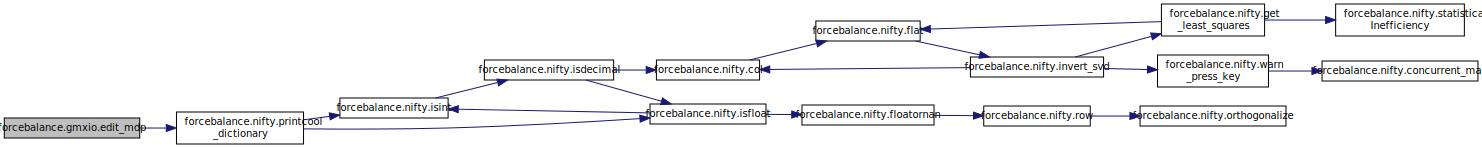
\includegraphics[width=350pt]{namespaceforcebalance_1_1gmxio_acc5bef2c5c991cd70a948a1dd43ef6a6_cgraph}
\end{center}
\end{figure}


\hypertarget{namespaceforcebalance_1_1gmxio_a29af6ace00d7e58258e0a854ca13d954}{\index{forcebalance\-::gmxio@{forcebalance\-::gmxio}!parse\-\_\-atomtype\-\_\-line@{parse\-\_\-atomtype\-\_\-line}}
\index{parse\-\_\-atomtype\-\_\-line@{parse\-\_\-atomtype\-\_\-line}!forcebalance::gmxio@{forcebalance\-::gmxio}}
\paragraph[{parse\-\_\-atomtype\-\_\-line}]{\setlength{\rightskip}{0pt plus 5cm}def forcebalance.\-gmxio.\-parse\-\_\-atomtype\-\_\-line (
\begin{DoxyParamCaption}
\item[{}]{line}
\end{DoxyParamCaption}
)}}\label{namespaceforcebalance_1_1gmxio_a29af6ace00d7e58258e0a854ca13d954}


Parses the 'atomtype' line. 

Parses lines like this\-:\par
 {\ttfamily  opls\-\_\-135 C\-T 6 12.\-0107 0.\-0000 A 3.\-5000e-\/01 2.\-7614e-\/01\par
 C 12.\-0107 0.\-0000 A 3.\-7500e-\/01 4.\-3932e-\/01\par
 Na 11 22.\-9897 0.\-0000 A 6.\-068128070229e+03 2.\-662662556402e+01 0.\-0000e+00 ; P\-A\-R\-M 5 6\par
 } Look at all the variety!


\begin{DoxyParams}[1]{Parameters}
\mbox{\tt in}  & {\em line} & Input line. \\
\hline
\end{DoxyParams}
\begin{DoxyReturn}{Returns}
answer Dictionary containing\-:\par
 atom type\par
 bonded atom type (if any)\par
 atomic number (if any)\par
 atomic mass\par
 charge\par
 particle type\par
 force field parameters\par
 number of optional fields 
\end{DoxyReturn}


Definition at line 183 of file gmxio.\-py.



Here is the call graph for this function\-:\nopagebreak
\begin{figure}[H]
\begin{center}
\leavevmode
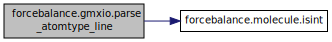
\includegraphics[width=350pt]{namespaceforcebalance_1_1gmxio_a29af6ace00d7e58258e0a854ca13d954_cgraph}
\end{center}
\end{figure}


\hypertarget{namespaceforcebalance_1_1gmxio_acac8488f29b62fb0d4cb54bb5a041026}{\index{forcebalance\-::gmxio@{forcebalance\-::gmxio}!rm\-\_\-gmx\-\_\-baks@{rm\-\_\-gmx\-\_\-baks}}
\index{rm\-\_\-gmx\-\_\-baks@{rm\-\_\-gmx\-\_\-baks}!forcebalance::gmxio@{forcebalance\-::gmxio}}
\paragraph[{rm\-\_\-gmx\-\_\-baks}]{\setlength{\rightskip}{0pt plus 5cm}def forcebalance.\-gmxio.\-rm\-\_\-gmx\-\_\-baks (
\begin{DoxyParamCaption}
\item[{}]{dir}
\end{DoxyParamCaption}
)}}\label{namespaceforcebalance_1_1gmxio_acac8488f29b62fb0d4cb54bb5a041026}


Definition at line 430 of file gmxio.\-py.



\subsubsection{Variable Documentation}
\hypertarget{namespaceforcebalance_1_1gmxio_aef89ff391902f81feb14e28ec301296c}{\index{forcebalance\-::gmxio@{forcebalance\-::gmxio}!aftypes@{aftypes}}
\index{aftypes@{aftypes}!forcebalance::gmxio@{forcebalance\-::gmxio}}
\paragraph[{aftypes}]{\setlength{\rightskip}{0pt plus 5cm}list forcebalance.\-gmxio.\-aftypes}}\label{namespaceforcebalance_1_1gmxio_aef89ff391902f81feb14e28ec301296c}
{\bfseries Initial value\-:}
\begin{DoxyCode}
1 = [\textcolor{keywordtype}{None}, \textcolor{stringliteral}{'ANGLES'}, \textcolor{stringliteral}{'G96ANGLES'}, \textcolor{stringliteral}{'CROSS\_BOND\_BOND'},
2            \textcolor{stringliteral}{'CROSS\_BOND\_ANGLE'}, \textcolor{stringliteral}{'UREY\_BRADLEY'}, \textcolor{stringliteral}{'QANGLES'}]
\end{DoxyCode}


Angle interaction function types. 



Definition at line 93 of file gmxio.\-py.

\hypertarget{namespaceforcebalance_1_1gmxio_a49a34b85d405c9286ceec1e6f088069f}{\index{forcebalance\-::gmxio@{forcebalance\-::gmxio}!bftypes@{bftypes}}
\index{bftypes@{bftypes}!forcebalance::gmxio@{forcebalance\-::gmxio}}
\paragraph[{bftypes}]{\setlength{\rightskip}{0pt plus 5cm}list forcebalance.\-gmxio.\-bftypes = \mbox{[}None, 'B\-O\-N\-D\-S', 'G96\-B\-O\-N\-D\-S', 'M\-O\-R\-S\-E'\mbox{]}}}\label{namespaceforcebalance_1_1gmxio_a49a34b85d405c9286ceec1e6f088069f}


Bonded interaction function types. 



Definition at line 91 of file gmxio.\-py.

\hypertarget{namespaceforcebalance_1_1gmxio_acd9fed3887161c6386506563fd4f3534}{\index{forcebalance\-::gmxio@{forcebalance\-::gmxio}!dftypes@{dftypes}}
\index{dftypes@{dftypes}!forcebalance::gmxio@{forcebalance\-::gmxio}}
\paragraph[{dftypes}]{\setlength{\rightskip}{0pt plus 5cm}list forcebalance.\-gmxio.\-dftypes = \mbox{[}None, 'P\-D\-I\-H\-S', 'I\-D\-I\-H\-S', 'R\-B\-D\-I\-H\-S', 'P\-I\-M\-P\-D\-I\-H\-S', 'F\-O\-U\-R\-D\-I\-H\-S', None, None, 'T\-A\-B\-D\-I\-H\-S', 'P\-D\-I\-H\-M\-U\-L\-S'\mbox{]}}}\label{namespaceforcebalance_1_1gmxio_acd9fed3887161c6386506563fd4f3534}


Dihedral interaction function types. 



Definition at line 96 of file gmxio.\-py.

\hypertarget{namespaceforcebalance_1_1gmxio_a179cbde2e55b4c025af89b225612d6e1}{\index{forcebalance\-::gmxio@{forcebalance\-::gmxio}!fdict@{fdict}}
\index{fdict@{fdict}!forcebalance::gmxio@{forcebalance\-::gmxio}}
\paragraph[{fdict}]{\setlength{\rightskip}{0pt plus 5cm}dictionary forcebalance.\-gmxio.\-fdict}}\label{namespaceforcebalance_1_1gmxio_a179cbde2e55b4c025af89b225612d6e1}
{\bfseries Initial value\-:}
\begin{DoxyCode}
1 = \{
2     \textcolor{stringliteral}{'atomtypes'}     : nftypes,
3     \textcolor{stringliteral}{'nonbond\_params'}: pftypes,
4     \textcolor{stringliteral}{'bonds'}         : bftypes,
5     \textcolor{stringliteral}{'bondtypes'}     : bftypes,
6     \textcolor{stringliteral}{'angles'}        : aftypes,
7     \textcolor{stringliteral}{'angletypes'}    : aftypes,
8     \textcolor{stringliteral}{'dihedrals'}     : dftypes,
9     \textcolor{stringliteral}{'dihedraltypes'} : dftypes,
10     \textcolor{stringliteral}{'virtual\_sites2'}: [\textcolor{stringliteral}{'NONE'},\textcolor{stringliteral}{'VSITE2'}],
11     \textcolor{stringliteral}{'virtual\_sites3'}: [\textcolor{stringliteral}{'NONE'},\textcolor{stringliteral}{'VSITE3'},\textcolor{stringliteral}{'VSITE3FD'},\textcolor{stringliteral}{'VSITE3FAD'},\textcolor{stringliteral}{'VSITE3OUT'}],
12     \textcolor{stringliteral}{'virtual\_sites4'}: [\textcolor{stringliteral}{'NONE'},\textcolor{stringliteral}{'VSITE4FD'},\textcolor{stringliteral}{'VSITE4FDN'}]
13     \}
\end{DoxyCode}


Section -\/$>$ Interaction type dictionary. 

Based on the section you're in and the integer given on the current line, this looks up the 'interaction type' -\/ for example, within bonded interactions there are four interaction types\-: harmonic, G96, Morse, and quartic interactions. 

Definition at line 104 of file gmxio.\-py.

\hypertarget{namespaceforcebalance_1_1gmxio_ac10457054444ca04e0a265665afc2512}{\index{forcebalance\-::gmxio@{forcebalance\-::gmxio}!logger@{logger}}
\index{logger@{logger}!forcebalance::gmxio@{forcebalance\-::gmxio}}
\paragraph[{logger}]{\setlength{\rightskip}{0pt plus 5cm}tuple forcebalance.\-gmxio.\-logger = get\-Logger(\-\_\-\-\_\-name\-\_\-\-\_\-)}}\label{namespaceforcebalance_1_1gmxio_ac10457054444ca04e0a265665afc2512}


Definition at line 28 of file gmxio.\-py.

\hypertarget{namespaceforcebalance_1_1gmxio_a337bc61280b58a43319380dec9c5529a}{\index{forcebalance\-::gmxio@{forcebalance\-::gmxio}!nftypes@{nftypes}}
\index{nftypes@{nftypes}!forcebalance::gmxio@{forcebalance\-::gmxio}}
\paragraph[{nftypes}]{\setlength{\rightskip}{0pt plus 5cm}list forcebalance.\-gmxio.\-nftypes = \mbox{[}None, 'V\-D\-W', 'V\-D\-W\-\_\-\-B\-H\-A\-M'\mbox{]}}}\label{namespaceforcebalance_1_1gmxio_a337bc61280b58a43319380dec9c5529a}


Vd\-W interaction function types. 



Definition at line 87 of file gmxio.\-py.

\hypertarget{namespaceforcebalance_1_1gmxio_ae845e0b923ecde16c79f2742b94534a6}{\index{forcebalance\-::gmxio@{forcebalance\-::gmxio}!pdict@{pdict}}
\index{pdict@{pdict}!forcebalance::gmxio@{forcebalance\-::gmxio}}
\paragraph[{pdict}]{\setlength{\rightskip}{0pt plus 5cm}dictionary forcebalance.\-gmxio.\-pdict}}\label{namespaceforcebalance_1_1gmxio_ae845e0b923ecde16c79f2742b94534a6}


Interaction type -\/$>$ Parameter Dictionary. 

A list of supported G\-R\-O\-M\-A\-C\-S interaction types in force matching. The keys in this dictionary (e.\-g. 'B\-O\-N\-D\-S','A\-N\-G\-L\-E\-S') are values in the interaction type dictionary. As the program loops through the force field file, it first looks up the interaction types in 'fdict' and then goes here to do the parameter lookup by field. \begin{DoxyRefDesc}{Todo}
\item[\hyperlink{todo__todo000010}{Todo}]This needs to become more flexible because the parameter isn't always in the same field. Still need to figure out how to do this. 

How about making the P\-D\-I\-H\-S less ugly? \end{DoxyRefDesc}


Definition at line 127 of file gmxio.\-py.

\hypertarget{namespaceforcebalance_1_1gmxio_a59695b79df36efbe64ac88fd64bfb366}{\index{forcebalance\-::gmxio@{forcebalance\-::gmxio}!pftypes@{pftypes}}
\index{pftypes@{pftypes}!forcebalance::gmxio@{forcebalance\-::gmxio}}
\paragraph[{pftypes}]{\setlength{\rightskip}{0pt plus 5cm}list forcebalance.\-gmxio.\-pftypes = \mbox{[}None, 'V\-P\-A\-I\-R', 'V\-P\-A\-I\-R\-\_\-\-B\-H\-A\-M'\mbox{]}}}\label{namespaceforcebalance_1_1gmxio_a59695b79df36efbe64ac88fd64bfb366}


Pairwise interaction function types. 



Definition at line 89 of file gmxio.\-py.

\hypertarget{namespaceforcebalance_1_1gmxio_a35d747dea4a5446d049d901e782feaa2}{\index{forcebalance\-::gmxio@{forcebalance\-::gmxio}!shot\-\_\-mdp@{shot\-\_\-mdp}}
\index{shot\-\_\-mdp@{shot\-\_\-mdp}!forcebalance::gmxio@{forcebalance\-::gmxio}}
\paragraph[{shot\-\_\-mdp}]{\setlength{\rightskip}{0pt plus 5cm}string forcebalance.\-gmxio.\-shot\-\_\-mdp}}\label{namespaceforcebalance_1_1gmxio_a35d747dea4a5446d049d901e782feaa2}
{\bfseries Initial value\-:}
\begin{DoxyCode}
1 = \textcolor{stringliteral}{"""integrator = md}
2 \textcolor{stringliteral}{dt              = 0.001}
3 \textcolor{stringliteral}{nsteps          = 0}
4 \textcolor{stringliteral}{nstxout         = 0}
5 \textcolor{stringliteral}{nstfout         = 1}
6 \textcolor{stringliteral}{nstenergy       = 1}
7 \textcolor{stringliteral}{nstxtcout       = 0}
8 \textcolor{stringliteral}{xtc\_grps        = System}
9 \textcolor{stringliteral}{energygrps      = System}
10 \textcolor{stringliteral}{}
11 \textcolor{stringliteral}{nstlist         = 0}
12 \textcolor{stringliteral}{ns\_type         = simple}
13 \textcolor{stringliteral}{rlist           = 0.0}
14 \textcolor{stringliteral}{vdwtype         = cut-off}
15 \textcolor{stringliteral}{coulombtype     = cut-off}
16 \textcolor{stringliteral}{rcoulomb        = 0.0}
17 \textcolor{stringliteral}{rvdw            = 0.0}
18 \textcolor{stringliteral}{constraints     = none}
19 \textcolor{stringliteral}{pbc             = no}
20 \textcolor{stringliteral}{"""}
\end{DoxyCode}


Definition at line 438 of file gmxio.\-py.


\hypertarget{namespaceforcebalance_1_1interaction}{}\subsection{forcebalance.\+interaction Namespace Reference}
\label{namespaceforcebalance_1_1interaction}\index{forcebalance.\+interaction@{forcebalance.\+interaction}}


Interaction energy fitting module.  




\subsubsection{Detailed Description}
Interaction energy fitting module. 

\begin{DoxyAuthor}{Author}
Lee-\/\+Ping Wang 
\end{DoxyAuthor}
\begin{DoxyDate}{Date}
05/2012 
\end{DoxyDate}

\hypertarget{namespaceforcebalance_1_1leastsq}{\subsection{forcebalance.\-leastsq Namespace Reference}
\label{namespaceforcebalance_1_1leastsq}\index{forcebalance.\-leastsq@{forcebalance.\-leastsq}}
}
\subsubsection*{Classes}
\begin{DoxyCompactItemize}
\item 
class \hyperlink{classforcebalance_1_1leastsq_1_1LeastSquares}{Least\-Squares}
\begin{DoxyCompactList}\small\item\em Subclass of Target for general least squares fitting. \end{DoxyCompactList}\end{DoxyCompactItemize}
\subsubsection*{Functions}
\begin{DoxyCompactItemize}
\item 
def \hyperlink{namespaceforcebalance_1_1leastsq_a8e7ef329e27aff738bc91dd79bd2dd1c}{Check\-Basis}
\item 
def \hyperlink{namespaceforcebalance_1_1leastsq_ad9d0036b0003e0245608ffb192c7c60c}{Last\-Mvals}
\end{DoxyCompactItemize}
\subsubsection*{Variables}
\begin{DoxyCompactItemize}
\item 
tuple \hyperlink{namespaceforcebalance_1_1leastsq_ab5873c70f3da934d9c5c78ca9c7ca8d0}{logger} = get\-Logger(\-\_\-\-\_\-name\-\_\-\-\_\-)
\item 
\hyperlink{namespaceforcebalance_1_1leastsq_a87815b7768ddc6d9caf7fa3c804fe303}{C\-H\-E\-C\-K\-\_\-\-B\-A\-S\-I\-S} = False
\item 
\hyperlink{namespaceforcebalance_1_1leastsq_a037a62063d126288c2df0f4e0cd5085a}{L\-A\-S\-T\-\_\-\-M\-V\-A\-L\-S} = None
\end{DoxyCompactItemize}


\subsubsection{Function Documentation}
\hypertarget{namespaceforcebalance_1_1leastsq_a8e7ef329e27aff738bc91dd79bd2dd1c}{\index{forcebalance\-::leastsq@{forcebalance\-::leastsq}!Check\-Basis@{Check\-Basis}}
\index{Check\-Basis@{Check\-Basis}!forcebalance::leastsq@{forcebalance\-::leastsq}}
\paragraph[{Check\-Basis}]{\setlength{\rightskip}{0pt plus 5cm}def forcebalance.\-leastsq.\-Check\-Basis (
\begin{DoxyParamCaption}
{}
\end{DoxyParamCaption}
)}}\label{namespaceforcebalance_1_1leastsq_a8e7ef329e27aff738bc91dd79bd2dd1c}


Definition at line 24 of file leastsq.\-py.

\hypertarget{namespaceforcebalance_1_1leastsq_ad9d0036b0003e0245608ffb192c7c60c}{\index{forcebalance\-::leastsq@{forcebalance\-::leastsq}!Last\-Mvals@{Last\-Mvals}}
\index{Last\-Mvals@{Last\-Mvals}!forcebalance::leastsq@{forcebalance\-::leastsq}}
\paragraph[{Last\-Mvals}]{\setlength{\rightskip}{0pt plus 5cm}def forcebalance.\-leastsq.\-Last\-Mvals (
\begin{DoxyParamCaption}
{}
\end{DoxyParamCaption}
)}}\label{namespaceforcebalance_1_1leastsq_ad9d0036b0003e0245608ffb192c7c60c}


Definition at line 29 of file leastsq.\-py.



\subsubsection{Variable Documentation}
\hypertarget{namespaceforcebalance_1_1leastsq_a87815b7768ddc6d9caf7fa3c804fe303}{\index{forcebalance\-::leastsq@{forcebalance\-::leastsq}!C\-H\-E\-C\-K\-\_\-\-B\-A\-S\-I\-S@{C\-H\-E\-C\-K\-\_\-\-B\-A\-S\-I\-S}}
\index{C\-H\-E\-C\-K\-\_\-\-B\-A\-S\-I\-S@{C\-H\-E\-C\-K\-\_\-\-B\-A\-S\-I\-S}!forcebalance::leastsq@{forcebalance\-::leastsq}}
\paragraph[{C\-H\-E\-C\-K\-\_\-\-B\-A\-S\-I\-S}]{\setlength{\rightskip}{0pt plus 5cm}forcebalance.\-leastsq.\-C\-H\-E\-C\-K\-\_\-\-B\-A\-S\-I\-S = False}}\label{namespaceforcebalance_1_1leastsq_a87815b7768ddc6d9caf7fa3c804fe303}


Definition at line 23 of file leastsq.\-py.

\hypertarget{namespaceforcebalance_1_1leastsq_a037a62063d126288c2df0f4e0cd5085a}{\index{forcebalance\-::leastsq@{forcebalance\-::leastsq}!L\-A\-S\-T\-\_\-\-M\-V\-A\-L\-S@{L\-A\-S\-T\-\_\-\-M\-V\-A\-L\-S}}
\index{L\-A\-S\-T\-\_\-\-M\-V\-A\-L\-S@{L\-A\-S\-T\-\_\-\-M\-V\-A\-L\-S}!forcebalance::leastsq@{forcebalance\-::leastsq}}
\paragraph[{L\-A\-S\-T\-\_\-\-M\-V\-A\-L\-S}]{\setlength{\rightskip}{0pt plus 5cm}forcebalance.\-leastsq.\-L\-A\-S\-T\-\_\-\-M\-V\-A\-L\-S = None}}\label{namespaceforcebalance_1_1leastsq_a037a62063d126288c2df0f4e0cd5085a}


Definition at line 28 of file leastsq.\-py.

\hypertarget{namespaceforcebalance_1_1leastsq_ab5873c70f3da934d9c5c78ca9c7ca8d0}{\index{forcebalance\-::leastsq@{forcebalance\-::leastsq}!logger@{logger}}
\index{logger@{logger}!forcebalance::leastsq@{forcebalance\-::leastsq}}
\paragraph[{logger}]{\setlength{\rightskip}{0pt plus 5cm}tuple forcebalance.\-leastsq.\-logger = get\-Logger(\-\_\-\-\_\-name\-\_\-\-\_\-)}}\label{namespaceforcebalance_1_1leastsq_ab5873c70f3da934d9c5c78ca9c7ca8d0}


Definition at line 21 of file leastsq.\-py.


\hypertarget{namespaceforcebalance_1_1lipid}{}\subsection{forcebalance.\+lipid Namespace Reference}
\label{namespaceforcebalance_1_1lipid}\index{forcebalance.\+lipid@{forcebalance.\+lipid}}


Matching of lipid bulk properties.  




\subsubsection{Detailed Description}
Matching of lipid bulk properties. 

Under development.

author Lee-\/\+Ping Wang \begin{DoxyDate}{Date}
04/2012 
\end{DoxyDate}

\hypertarget{namespaceforcebalance_1_1liquid}{\subsection{forcebalance.\-liquid Namespace Reference}
\label{namespaceforcebalance_1_1liquid}\index{forcebalance.\-liquid@{forcebalance.\-liquid}}
}

\hypertarget{namespaceforcebalance_1_1Mol2}{\subsection{forcebalance.\-Mol2 Namespace Reference}
\label{namespaceforcebalance_1_1Mol2}\index{forcebalance.\-Mol2@{forcebalance.\-Mol2}}
}

\hypertarget{namespaceforcebalance_1_1mol2io}{\subsection{forcebalance.\-mol2io Namespace Reference}
\label{namespaceforcebalance_1_1mol2io}\index{forcebalance.\-mol2io@{forcebalance.\-mol2io}}
}

\hypertarget{namespaceforcebalance_1_1molecule}{\subsection{forcebalance.\-molecule Namespace Reference}
\label{namespaceforcebalance_1_1molecule}\index{forcebalance.\-molecule@{forcebalance.\-molecule}}
}
\subsubsection*{Classes}
\begin{DoxyCompactItemize}
\item 
class \hyperlink{classforcebalance_1_1molecule_1_1MolfileTimestep}{Molfile\-Timestep}
\begin{DoxyCompactList}\small\item\em Wrapper for the timestep C structure used in molfile plugins. \end{DoxyCompactList}\item 
class \hyperlink{classforcebalance_1_1molecule_1_1Molecule}{Molecule}
\begin{DoxyCompactList}\small\item\em Lee-\/\-Ping's general file format conversion class. \end{DoxyCompactList}\end{DoxyCompactItemize}
\subsubsection*{Functions}
\begin{DoxyCompactItemize}
\item 
def \hyperlink{namespaceforcebalance_1_1molecule_af28de4693e5b8e82df900d0ac3c6c370}{get\-Element}
\item 
def \hyperlink{namespaceforcebalance_1_1molecule_a7429f0c377d6396711c128f6590ef810}{elem\-\_\-from\-\_\-atomname}
\begin{DoxyCompactList}\small\item\em Given an atom name, attempt to get the element in most cases. \end{DoxyCompactList}\item 
def \hyperlink{namespaceforcebalance_1_1molecule_ab8464fea13fad2a506792c2f1d7c93f3}{nodematch}
\item 
def \hyperlink{namespaceforcebalance_1_1molecule_a0dd31eff88d2bed0884ab21a13261d42}{isint}
\begin{DoxyCompactList}\small\item\em O\-N\-L\-Y matches integers! If you have a decimal point? None shall pass! \end{DoxyCompactList}\item 
def \hyperlink{namespaceforcebalance_1_1molecule_afe989ffd119568047fc8265b1d329a70}{isfloat}
\begin{DoxyCompactList}\small\item\em Matches A\-N\-Y number; it can be a decimal, scientific notation, integer, or what have you. \end{DoxyCompactList}\item 
def \hyperlink{namespaceforcebalance_1_1molecule_a0a6e3e79b04534bf2e83d09def189444}{Build\-Lattice\-From\-Lengths\-Angles}
\begin{DoxyCompactList}\small\item\em This function takes in three lattice lengths and three lattice angles, and tries to return a complete box specification. \end{DoxyCompactList}\item 
def \hyperlink{namespaceforcebalance_1_1molecule_a29fb1ac9324f4280f07c65baea339989}{Build\-Lattice\-From\-Vectors}
\begin{DoxyCompactList}\small\item\em This function takes in three lattice vectors and tries to return a complete box specification. \end{DoxyCompactList}\item 
def \hyperlink{namespaceforcebalance_1_1molecule_a2eba3cad44138b3b10ea883240888412}{format\-\_\-xyz\-\_\-coord}
\begin{DoxyCompactList}\small\item\em Print a line consisting of (element, x, y, z) in accordance with .xyz file format. \end{DoxyCompactList}\item 
def \hyperlink{namespaceforcebalance_1_1molecule_a41c13064e4285973aa6c49369d3d3390}{format\-\_\-gro\-\_\-coord}
\begin{DoxyCompactList}\small\item\em Print a line in accordance with .gro file format, with six decimal points of precision. \end{DoxyCompactList}\item 
def \hyperlink{namespaceforcebalance_1_1molecule_a4948e4662b8d2c8d515427d1bbb3d01e}{format\-\_\-xyzgen\-\_\-coord}
\begin{DoxyCompactList}\small\item\em Print a line consisting of (element, p, q, r, s, t, ...) where (p, q, r) are arbitrary atom-\/wise data (this might happen, for instance, with atomic charges) \end{DoxyCompactList}\item 
def \hyperlink{namespaceforcebalance_1_1molecule_ae25aa5331b3a2dd0e9d1e184380357db}{format\-\_\-gro\-\_\-box}
\begin{DoxyCompactList}\small\item\em Print a line corresponding to the box vector in accordance with .gro file format. \end{DoxyCompactList}\item 
def \hyperlink{namespaceforcebalance_1_1molecule_a12b7bb398c2fa49a223f258ec7737483}{is\-\_\-gro\-\_\-coord}
\begin{DoxyCompactList}\small\item\em Determines whether a line contains G\-R\-O\-M\-A\-C\-S data or not. \end{DoxyCompactList}\item 
def \hyperlink{namespaceforcebalance_1_1molecule_a838d85848bd817e801d0f5f6502217ef}{is\-\_\-charmm\-\_\-coord}
\begin{DoxyCompactList}\small\item\em Determines whether a line contains C\-H\-A\-R\-M\-M data or not. \end{DoxyCompactList}\item 
def \hyperlink{namespaceforcebalance_1_1molecule_aafc8c924eed4480fed8ddc9c474d3bc1}{is\-\_\-gro\-\_\-box}
\begin{DoxyCompactList}\small\item\em Determines whether a line contains a G\-R\-O\-M\-A\-C\-S box vector or not. \end{DoxyCompactList}\item 
def \hyperlink{namespaceforcebalance_1_1molecule_a4cdb2086978b281ed84cd66179c3f5b2}{add\-\_\-strip\-\_\-to\-\_\-mat}
\item 
def \hyperlink{namespaceforcebalance_1_1molecule_a58c3f09152db4d1c6e1db9df29c60c43}{pvec}
\item 
def \hyperlink{namespaceforcebalance_1_1molecule_a7fe52c2928c7b0329882541bef2e34cd}{grouper}
\begin{DoxyCompactList}\small\item\em Groups a big long iterable into groups of ten or what have you. \end{DoxyCompactList}\item 
def \hyperlink{namespaceforcebalance_1_1molecule_a5f529179461765fadbd0a742cdc2c677}{even\-\_\-list}
\begin{DoxyCompactList}\small\item\em Creates a list of number sequences divided as evenly as possible. \end{DoxyCompactList}\item 
def \hyperlink{namespaceforcebalance_1_1molecule_a5b50df23cc4d0e617fdc56538f0bea63}{both}
\item 
def \hyperlink{namespaceforcebalance_1_1molecule_a6f7c6217b1c64da309a8abd21dfdcf08}{diff}
\item 
def \hyperlink{namespaceforcebalance_1_1molecule_a75775be6563ad7f10695a9a45ff49ba9}{either}
\item 
def \hyperlink{namespaceforcebalance_1_1molecule_af02bf73765f34bbef81c4a5b000b86ce}{Euler\-Matrix}
\begin{DoxyCompactList}\small\item\em Constructs an Euler matrix from three Euler angles. \end{DoxyCompactList}\item 
def \hyperlink{namespaceforcebalance_1_1molecule_a8fcbb4a2b3470a85d25699b6f28a54fc}{Compute\-Overlap}
\begin{DoxyCompactList}\small\item\em Computes an 'overlap' between two molecules based on some fictitious density. \end{DoxyCompactList}\item 
def \hyperlink{namespaceforcebalance_1_1molecule_a9a58eb1746e51420f50da3f3a6d51485}{Align\-To\-Density}
\begin{DoxyCompactList}\small\item\em Computes a \char`\"{}overlap density\char`\"{} from two frames. \end{DoxyCompactList}\item 
def \hyperlink{namespaceforcebalance_1_1molecule_aa9ad9b92efa7bd3c1d589d62bbb8108e}{Align\-To\-Moments}
\begin{DoxyCompactList}\small\item\em Pre-\/aligns molecules to 'moment of inertia'. \end{DoxyCompactList}\item 
def \hyperlink{namespaceforcebalance_1_1molecule_a08840b73e95bf34bf9ca7ea36ad0492d}{get\-\_\-rotate\-\_\-translate}
\item 
def \hyperlink{namespaceforcebalance_1_1molecule_ae76fc5d05f43acc6006a4d1733818d71}{cartesian\-\_\-product2}
\begin{DoxyCompactList}\small\item\em Form a Cartesian product of two Num\-Py arrays. \end{DoxyCompactList}\item 
def \hyperlink{namespaceforcebalance_1_1molecule_ab9cb167fbbd809aedcf8c7434d405547}{main}
\end{DoxyCompactItemize}
\subsubsection*{Variables}
\begin{DoxyCompactItemize}
\item 
tuple \hyperlink{namespaceforcebalance_1_1molecule_a0044fa397e0923635a8b3e9625aa70f7}{Frame\-Variable\-Names}
\item 
tuple \hyperlink{namespaceforcebalance_1_1molecule_a5daa68e835dcb9877d6c3f2fb559b54b}{Atom\-Variable\-Names} = set(\mbox{[}'elem', 'partial\-\_\-charge', 'atomname', 'atomtype', 'tinkersuf', 'resid', 'resname', 'qcsuf', 'qm\-\_\-ghost', 'chain', 'altloc', 'icode'\mbox{]})
\item 
tuple \hyperlink{namespaceforcebalance_1_1molecule_a38e1c99e9567fe42b792af43db9b7488}{Meta\-Variable\-Names} = set(\mbox{[}'fnm', 'ftype', 'qcrems', 'qctemplate', 'charge', 'mult', 'bonds'\mbox{]})
\item 
tuple \hyperlink{namespaceforcebalance_1_1molecule_ab67efeab6049ec1f416b9ad1eed6ffcc}{Quantum\-Variable\-Names} = set(\mbox{[}'qcrems', 'qctemplate', 'charge', 'mult', 'qcsuf', 'qm\-\_\-ghost'\mbox{]})
\item 
\hyperlink{namespaceforcebalance_1_1molecule_a8fcfb88fe12a9256b61980f3d4fe3b63}{All\-Variable\-Names} = \hyperlink{namespaceforcebalance_1_1molecule_ab67efeab6049ec1f416b9ad1eed6ffcc}{Quantum\-Variable\-Names}$|$\hyperlink{namespaceforcebalance_1_1molecule_a5daa68e835dcb9877d6c3f2fb559b54b}{Atom\-Variable\-Names}$|$\hyperlink{namespaceforcebalance_1_1molecule_a38e1c99e9567fe42b792af43db9b7488}{Meta\-Variable\-Names}$|$\hyperlink{namespaceforcebalance_1_1molecule_a0044fa397e0923635a8b3e9625aa70f7}{Frame\-Variable\-Names}
\item 
list \hyperlink{namespaceforcebalance_1_1molecule_a74f55a89a14ca676b5a06441d1fdab19}{Radii}
\item 
list \hyperlink{namespaceforcebalance_1_1molecule_a1c99a11e8a749468698c9af6361a8a4c}{Elements}
\item 
tuple \hyperlink{namespaceforcebalance_1_1molecule_adc5040ec456762f2ac240fb08febbfdd}{Periodic\-Table}
\item 
float \hyperlink{namespaceforcebalance_1_1molecule_a76af9edfbaaa8999680e32aafe1b1b61}{bohrang} = 0.\-529177249
\begin{DoxyCompactList}\small\item\em One bohr equals this many angstroms. \end{DoxyCompactList}\item 
tuple \hyperlink{namespaceforcebalance_1_1molecule_a09d04113accea9c88b084051c5de29d1}{splitter} = re.\-compile(r'(\textbackslash{}s+$|$\textbackslash{}S+)')
\item 
tuple \hyperlink{namespaceforcebalance_1_1molecule_aa761cf1cf260e15d0b03a6f61569c840}{Box} = namedtuple('Box',\mbox{[}'a','b','c','alpha','beta','gamma','A','B','C','V'\mbox{]})
\item 
int \hyperlink{namespaceforcebalance_1_1molecule_a1ee5389ce8a9042e053c7972dbbfb005}{radian} = 180
\item 
\hyperlink{namespaceforcebalance_1_1molecule_a2986996d4f957928047df06fbec3717d}{Alive}
\end{DoxyCompactItemize}


\subsubsection{Function Documentation}
\hypertarget{namespaceforcebalance_1_1molecule_a4cdb2086978b281ed84cd66179c3f5b2}{\index{forcebalance\-::molecule@{forcebalance\-::molecule}!add\-\_\-strip\-\_\-to\-\_\-mat@{add\-\_\-strip\-\_\-to\-\_\-mat}}
\index{add\-\_\-strip\-\_\-to\-\_\-mat@{add\-\_\-strip\-\_\-to\-\_\-mat}!forcebalance::molecule@{forcebalance\-::molecule}}
\paragraph[{add\-\_\-strip\-\_\-to\-\_\-mat}]{\setlength{\rightskip}{0pt plus 5cm}def forcebalance.\-molecule.\-add\-\_\-strip\-\_\-to\-\_\-mat (
\begin{DoxyParamCaption}
\item[{}]{mat, }
\item[{}]{strip}
\end{DoxyParamCaption}
)}}\label{namespaceforcebalance_1_1molecule_a4cdb2086978b281ed84cd66179c3f5b2}


Definition at line 441 of file molecule.\-py.

\hypertarget{namespaceforcebalance_1_1molecule_a9a58eb1746e51420f50da3f3a6d51485}{\index{forcebalance\-::molecule@{forcebalance\-::molecule}!Align\-To\-Density@{Align\-To\-Density}}
\index{Align\-To\-Density@{Align\-To\-Density}!forcebalance::molecule@{forcebalance\-::molecule}}
\paragraph[{Align\-To\-Density}]{\setlength{\rightskip}{0pt plus 5cm}def forcebalance.\-molecule.\-Align\-To\-Density (
\begin{DoxyParamCaption}
\item[{}]{elem, }
\item[{}]{xyz1, }
\item[{}]{xyz2, }
\item[{}]{binary = {\ttfamily False}}
\end{DoxyParamCaption}
)}}\label{namespaceforcebalance_1_1molecule_a9a58eb1746e51420f50da3f3a6d51485}


Computes a \char`\"{}overlap density\char`\"{} from two frames. 

This function can be called by Align\-To\-Moments to get rid of inversion problems 

Definition at line 544 of file molecule.\-py.



Here is the call graph for this function\-:
\nopagebreak
\begin{figure}[H]
\begin{center}
\leavevmode
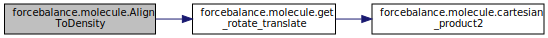
\includegraphics[width=350pt]{namespaceforcebalance_1_1molecule_a9a58eb1746e51420f50da3f3a6d51485_cgraph}
\end{center}
\end{figure}


\hypertarget{namespaceforcebalance_1_1molecule_aa9ad9b92efa7bd3c1d589d62bbb8108e}{\index{forcebalance\-::molecule@{forcebalance\-::molecule}!Align\-To\-Moments@{Align\-To\-Moments}}
\index{Align\-To\-Moments@{Align\-To\-Moments}!forcebalance::molecule@{forcebalance\-::molecule}}
\paragraph[{Align\-To\-Moments}]{\setlength{\rightskip}{0pt plus 5cm}def forcebalance.\-molecule.\-Align\-To\-Moments (
\begin{DoxyParamCaption}
\item[{}]{elem, }
\item[{}]{xyz1, }
\item[{}]{xyz2 = {\ttfamily None}}
\end{DoxyParamCaption}
)}}\label{namespaceforcebalance_1_1molecule_aa9ad9b92efa7bd3c1d589d62bbb8108e}


Pre-\/aligns molecules to 'moment of inertia'. 

If xyz2 is passed in, it will assume that xyz1 is already aligned to the moment of inertia, and it simply does 180-\/degree rotations to make sure nothing is inverted. 

Definition at line 556 of file molecule.\-py.

\hypertarget{namespaceforcebalance_1_1molecule_a5b50df23cc4d0e617fdc56538f0bea63}{\index{forcebalance\-::molecule@{forcebalance\-::molecule}!both@{both}}
\index{both@{both}!forcebalance::molecule@{forcebalance\-::molecule}}
\paragraph[{both}]{\setlength{\rightskip}{0pt plus 5cm}def forcebalance.\-molecule.\-both (
\begin{DoxyParamCaption}
\item[{}]{A, }
\item[{}]{B, }
\item[{}]{key}
\end{DoxyParamCaption}
)}}\label{namespaceforcebalance_1_1molecule_a5b50df23cc4d0e617fdc56538f0bea63}


Definition at line 479 of file molecule.\-py.

\hypertarget{namespaceforcebalance_1_1molecule_a0a6e3e79b04534bf2e83d09def189444}{\index{forcebalance\-::molecule@{forcebalance\-::molecule}!Build\-Lattice\-From\-Lengths\-Angles@{Build\-Lattice\-From\-Lengths\-Angles}}
\index{Build\-Lattice\-From\-Lengths\-Angles@{Build\-Lattice\-From\-Lengths\-Angles}!forcebalance::molecule@{forcebalance\-::molecule}}
\paragraph[{Build\-Lattice\-From\-Lengths\-Angles}]{\setlength{\rightskip}{0pt plus 5cm}def forcebalance.\-molecule.\-Build\-Lattice\-From\-Lengths\-Angles (
\begin{DoxyParamCaption}
\item[{}]{a, }
\item[{}]{b, }
\item[{}]{c, }
\item[{}]{alpha, }
\item[{}]{beta, }
\item[{}]{gamma}
\end{DoxyParamCaption}
)}}\label{namespaceforcebalance_1_1molecule_a0a6e3e79b04534bf2e83d09def189444}


This function takes in three lattice lengths and three lattice angles, and tries to return a complete box specification. 



Definition at line 261 of file molecule.\-py.



Here is the call graph for this function\-:
\nopagebreak
\begin{figure}[H]
\begin{center}
\leavevmode
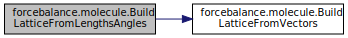
\includegraphics[width=350pt]{namespaceforcebalance_1_1molecule_a0a6e3e79b04534bf2e83d09def189444_cgraph}
\end{center}
\end{figure}


\hypertarget{namespaceforcebalance_1_1molecule_a29fb1ac9324f4280f07c65baea339989}{\index{forcebalance\-::molecule@{forcebalance\-::molecule}!Build\-Lattice\-From\-Vectors@{Build\-Lattice\-From\-Vectors}}
\index{Build\-Lattice\-From\-Vectors@{Build\-Lattice\-From\-Vectors}!forcebalance::molecule@{forcebalance\-::molecule}}
\paragraph[{Build\-Lattice\-From\-Vectors}]{\setlength{\rightskip}{0pt plus 5cm}def forcebalance.\-molecule.\-Build\-Lattice\-From\-Vectors (
\begin{DoxyParamCaption}
\item[{}]{v1, }
\item[{}]{v2, }
\item[{}]{v3}
\end{DoxyParamCaption}
)}}\label{namespaceforcebalance_1_1molecule_a29fb1ac9324f4280f07c65baea339989}


This function takes in three lattice vectors and tries to return a complete box specification. 

The hash function is something we can use to discard two things that are obviously not equal. Here we neglect the hash. Return a list of the sorted atom numbers in this graph. Return a string of atoms, which serves as a rudimentary 'fingerprint' \-: '99,100,103,151' . Return an array of the elements. For instance \mbox{[}'H' 'C' 'C' 'H'\mbox{]}. Create an Empirical Formula Get a list of the coordinates. 

Definition at line 276 of file molecule.\-py.

\hypertarget{namespaceforcebalance_1_1molecule_ae76fc5d05f43acc6006a4d1733818d71}{\index{forcebalance\-::molecule@{forcebalance\-::molecule}!cartesian\-\_\-product2@{cartesian\-\_\-product2}}
\index{cartesian\-\_\-product2@{cartesian\-\_\-product2}!forcebalance::molecule@{forcebalance\-::molecule}}
\paragraph[{cartesian\-\_\-product2}]{\setlength{\rightskip}{0pt plus 5cm}def forcebalance.\-molecule.\-cartesian\-\_\-product2 (
\begin{DoxyParamCaption}
\item[{}]{arrays}
\end{DoxyParamCaption}
)}}\label{namespaceforcebalance_1_1molecule_ae76fc5d05f43acc6006a4d1733818d71}


Form a Cartesian product of two Num\-Py arrays. 



Definition at line 617 of file molecule.\-py.

\hypertarget{namespaceforcebalance_1_1molecule_a8fcbb4a2b3470a85d25699b6f28a54fc}{\index{forcebalance\-::molecule@{forcebalance\-::molecule}!Compute\-Overlap@{Compute\-Overlap}}
\index{Compute\-Overlap@{Compute\-Overlap}!forcebalance::molecule@{forcebalance\-::molecule}}
\paragraph[{Compute\-Overlap}]{\setlength{\rightskip}{0pt plus 5cm}def forcebalance.\-molecule.\-Compute\-Overlap (
\begin{DoxyParamCaption}
\item[{}]{theta, }
\item[{}]{elem, }
\item[{}]{xyz1, }
\item[{}]{xyz2}
\end{DoxyParamCaption}
)}}\label{namespaceforcebalance_1_1molecule_a8fcbb4a2b3470a85d25699b6f28a54fc}


Computes an 'overlap' between two molecules based on some fictitious density. 

Good for fine-\/tuning alignment but gets stuck in local minima. 

Definition at line 527 of file molecule.\-py.



Here is the call graph for this function\-:
\nopagebreak
\begin{figure}[H]
\begin{center}
\leavevmode
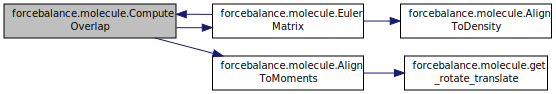
\includegraphics[width=350pt]{namespaceforcebalance_1_1molecule_a8fcbb4a2b3470a85d25699b6f28a54fc_cgraph}
\end{center}
\end{figure}


\hypertarget{namespaceforcebalance_1_1molecule_a6f7c6217b1c64da309a8abd21dfdcf08}{\index{forcebalance\-::molecule@{forcebalance\-::molecule}!diff@{diff}}
\index{diff@{diff}!forcebalance::molecule@{forcebalance\-::molecule}}
\paragraph[{diff}]{\setlength{\rightskip}{0pt plus 5cm}def forcebalance.\-molecule.\-diff (
\begin{DoxyParamCaption}
\item[{}]{A, }
\item[{}]{B, }
\item[{}]{key}
\end{DoxyParamCaption}
)}}\label{namespaceforcebalance_1_1molecule_a6f7c6217b1c64da309a8abd21dfdcf08}


Definition at line 482 of file molecule.\-py.

\hypertarget{namespaceforcebalance_1_1molecule_a75775be6563ad7f10695a9a45ff49ba9}{\index{forcebalance\-::molecule@{forcebalance\-::molecule}!either@{either}}
\index{either@{either}!forcebalance::molecule@{forcebalance\-::molecule}}
\paragraph[{either}]{\setlength{\rightskip}{0pt plus 5cm}def forcebalance.\-molecule.\-either (
\begin{DoxyParamCaption}
\item[{}]{A, }
\item[{}]{B, }
\item[{}]{key}
\end{DoxyParamCaption}
)}}\label{namespaceforcebalance_1_1molecule_a75775be6563ad7f10695a9a45ff49ba9}


Definition at line 490 of file molecule.\-py.

\hypertarget{namespaceforcebalance_1_1molecule_a7429f0c377d6396711c128f6590ef810}{\index{forcebalance\-::molecule@{forcebalance\-::molecule}!elem\-\_\-from\-\_\-atomname@{elem\-\_\-from\-\_\-atomname}}
\index{elem\-\_\-from\-\_\-atomname@{elem\-\_\-from\-\_\-atomname}!forcebalance::molecule@{forcebalance\-::molecule}}
\paragraph[{elem\-\_\-from\-\_\-atomname}]{\setlength{\rightskip}{0pt plus 5cm}def forcebalance.\-molecule.\-elem\-\_\-from\-\_\-atomname (
\begin{DoxyParamCaption}
\item[{}]{atomname}
\end{DoxyParamCaption}
)}}\label{namespaceforcebalance_1_1molecule_a7429f0c377d6396711c128f6590ef810}


Given an atom name, attempt to get the element in most cases. 



Definition at line 194 of file molecule.\-py.

\hypertarget{namespaceforcebalance_1_1molecule_af02bf73765f34bbef81c4a5b000b86ce}{\index{forcebalance\-::molecule@{forcebalance\-::molecule}!Euler\-Matrix@{Euler\-Matrix}}
\index{Euler\-Matrix@{Euler\-Matrix}!forcebalance::molecule@{forcebalance\-::molecule}}
\paragraph[{Euler\-Matrix}]{\setlength{\rightskip}{0pt plus 5cm}def forcebalance.\-molecule.\-Euler\-Matrix (
\begin{DoxyParamCaption}
\item[{}]{T1, }
\item[{}]{T2, }
\item[{}]{T3}
\end{DoxyParamCaption}
)}}\label{namespaceforcebalance_1_1molecule_af02bf73765f34bbef81c4a5b000b86ce}


Constructs an Euler matrix from three Euler angles. 



Definition at line 499 of file molecule.\-py.



Here is the call graph for this function\-:
\nopagebreak
\begin{figure}[H]
\begin{center}
\leavevmode
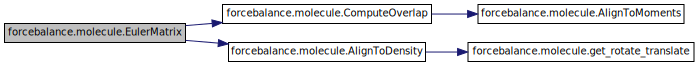
\includegraphics[width=350pt]{namespaceforcebalance_1_1molecule_af02bf73765f34bbef81c4a5b000b86ce_cgraph}
\end{center}
\end{figure}


\hypertarget{namespaceforcebalance_1_1molecule_a5f529179461765fadbd0a742cdc2c677}{\index{forcebalance\-::molecule@{forcebalance\-::molecule}!even\-\_\-list@{even\-\_\-list}}
\index{even\-\_\-list@{even\-\_\-list}!forcebalance::molecule@{forcebalance\-::molecule}}
\paragraph[{even\-\_\-list}]{\setlength{\rightskip}{0pt plus 5cm}def forcebalance.\-molecule.\-even\-\_\-list (
\begin{DoxyParamCaption}
\item[{}]{totlen, }
\item[{}]{splitsize}
\end{DoxyParamCaption}
)}}\label{namespaceforcebalance_1_1molecule_a5f529179461765fadbd0a742cdc2c677}


Creates a list of number sequences divided as evenly as possible. 



Definition at line 461 of file molecule.\-py.



Here is the call graph for this function\-:
\nopagebreak
\begin{figure}[H]
\begin{center}
\leavevmode
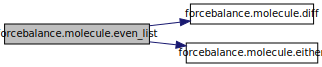
\includegraphics[width=350pt]{namespaceforcebalance_1_1molecule_a5f529179461765fadbd0a742cdc2c677_cgraph}
\end{center}
\end{figure}


\hypertarget{namespaceforcebalance_1_1molecule_ae25aa5331b3a2dd0e9d1e184380357db}{\index{forcebalance\-::molecule@{forcebalance\-::molecule}!format\-\_\-gro\-\_\-box@{format\-\_\-gro\-\_\-box}}
\index{format\-\_\-gro\-\_\-box@{format\-\_\-gro\-\_\-box}!forcebalance::molecule@{forcebalance\-::molecule}}
\paragraph[{format\-\_\-gro\-\_\-box}]{\setlength{\rightskip}{0pt plus 5cm}def forcebalance.\-molecule.\-format\-\_\-gro\-\_\-box (
\begin{DoxyParamCaption}
\item[{}]{box}
\end{DoxyParamCaption}
)}}\label{namespaceforcebalance_1_1molecule_ae25aa5331b3a2dd0e9d1e184380357db}


Print a line corresponding to the box vector in accordance with .gro file format. 


\begin{DoxyParams}[1]{Parameters}
\mbox{\tt in}  & {\em box} & Box Named\-Tuple \\
\hline
\end{DoxyParams}


Definition at line 392 of file molecule.\-py.



Here is the call graph for this function\-:
\nopagebreak
\begin{figure}[H]
\begin{center}
\leavevmode
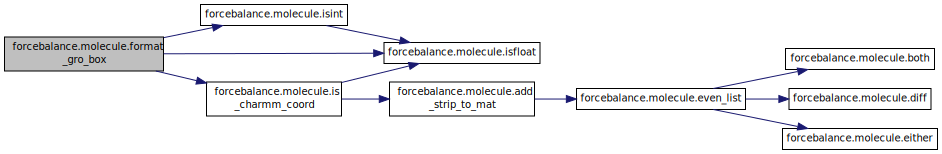
\includegraphics[width=350pt]{namespaceforcebalance_1_1molecule_ae25aa5331b3a2dd0e9d1e184380357db_cgraph}
\end{center}
\end{figure}


\hypertarget{namespaceforcebalance_1_1molecule_a41c13064e4285973aa6c49369d3d3390}{\index{forcebalance\-::molecule@{forcebalance\-::molecule}!format\-\_\-gro\-\_\-coord@{format\-\_\-gro\-\_\-coord}}
\index{format\-\_\-gro\-\_\-coord@{format\-\_\-gro\-\_\-coord}!forcebalance::molecule@{forcebalance\-::molecule}}
\paragraph[{format\-\_\-gro\-\_\-coord}]{\setlength{\rightskip}{0pt plus 5cm}def forcebalance.\-molecule.\-format\-\_\-gro\-\_\-coord (
\begin{DoxyParamCaption}
\item[{}]{resid, }
\item[{}]{resname, }
\item[{}]{aname, }
\item[{}]{seqno, }
\item[{}]{xyz}
\end{DoxyParamCaption}
)}}\label{namespaceforcebalance_1_1molecule_a41c13064e4285973aa6c49369d3d3390}


Print a line in accordance with .gro file format, with six decimal points of precision. 


\begin{DoxyParams}[1]{Parameters}
\mbox{\tt in}  & {\em resid} & The number of the residue that the atom belongs to \\
\hline
\mbox{\tt in}  & {\em resname} & The name of the residue that the atom belongs to \\
\hline
\mbox{\tt in}  & {\em aname} & The name of the atom \\
\hline
\mbox{\tt in}  & {\em seqno} & The sequential number of the atom \\
\hline
\mbox{\tt in}  & {\em xyz} & A 3-\/element array containing x, y, z coordinates of that atom \\
\hline
\end{DoxyParams}


Definition at line 371 of file molecule.\-py.



Here is the call graph for this function\-:
\nopagebreak
\begin{figure}[H]
\begin{center}
\leavevmode
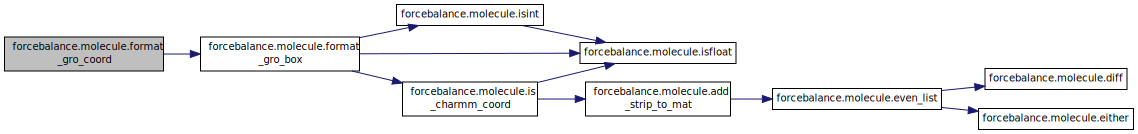
\includegraphics[width=350pt]{namespaceforcebalance_1_1molecule_a41c13064e4285973aa6c49369d3d3390_cgraph}
\end{center}
\end{figure}


\hypertarget{namespaceforcebalance_1_1molecule_a2eba3cad44138b3b10ea883240888412}{\index{forcebalance\-::molecule@{forcebalance\-::molecule}!format\-\_\-xyz\-\_\-coord@{format\-\_\-xyz\-\_\-coord}}
\index{format\-\_\-xyz\-\_\-coord@{format\-\_\-xyz\-\_\-coord}!forcebalance::molecule@{forcebalance\-::molecule}}
\paragraph[{format\-\_\-xyz\-\_\-coord}]{\setlength{\rightskip}{0pt plus 5cm}def forcebalance.\-molecule.\-format\-\_\-xyz\-\_\-coord (
\begin{DoxyParamCaption}
\item[{}]{element, }
\item[{}]{xyz, }
\item[{}]{tinker = {\ttfamily False}}
\end{DoxyParamCaption}
)}}\label{namespaceforcebalance_1_1molecule_a2eba3cad44138b3b10ea883240888412}


Print a line consisting of (element, x, y, z) in accordance with .xyz file format. 


\begin{DoxyParams}[1]{Parameters}
\mbox{\tt in}  & {\em element} & A chemical element of a single atom \\
\hline
\mbox{\tt in}  & {\em xyz} & A 3-\/element array containing x, y, z coordinates of that atom \\
\hline
\end{DoxyParams}


Definition at line 355 of file molecule.\-py.



Here is the call graph for this function\-:
\nopagebreak
\begin{figure}[H]
\begin{center}
\leavevmode
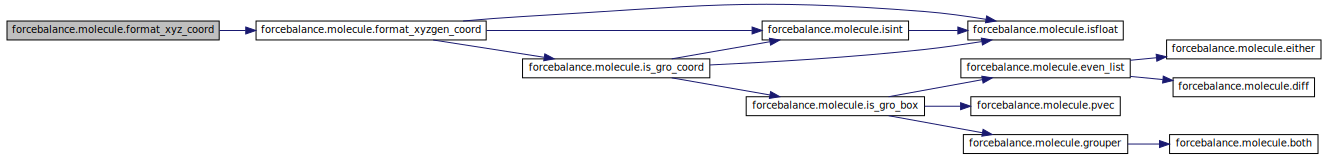
\includegraphics[width=350pt]{namespaceforcebalance_1_1molecule_a2eba3cad44138b3b10ea883240888412_cgraph}
\end{center}
\end{figure}


\hypertarget{namespaceforcebalance_1_1molecule_a4948e4662b8d2c8d515427d1bbb3d01e}{\index{forcebalance\-::molecule@{forcebalance\-::molecule}!format\-\_\-xyzgen\-\_\-coord@{format\-\_\-xyzgen\-\_\-coord}}
\index{format\-\_\-xyzgen\-\_\-coord@{format\-\_\-xyzgen\-\_\-coord}!forcebalance::molecule@{forcebalance\-::molecule}}
\paragraph[{format\-\_\-xyzgen\-\_\-coord}]{\setlength{\rightskip}{0pt plus 5cm}def forcebalance.\-molecule.\-format\-\_\-xyzgen\-\_\-coord (
\begin{DoxyParamCaption}
\item[{}]{element, }
\item[{}]{xyzgen}
\end{DoxyParamCaption}
)}}\label{namespaceforcebalance_1_1molecule_a4948e4662b8d2c8d515427d1bbb3d01e}


Print a line consisting of (element, p, q, r, s, t, ...) where (p, q, r) are arbitrary atom-\/wise data (this might happen, for instance, with atomic charges) 


\begin{DoxyParams}[1]{Parameters}
\mbox{\tt in}  & {\em element} & A chemical element of a single atom \\
\hline
\mbox{\tt in}  & {\em xyzgen} & A N-\/element array containing data for that atom \\
\hline
\end{DoxyParams}


Definition at line 383 of file molecule.\-py.



Here is the call graph for this function\-:
\nopagebreak
\begin{figure}[H]
\begin{center}
\leavevmode
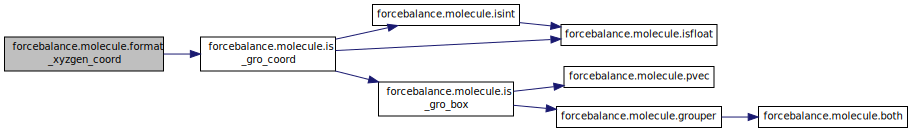
\includegraphics[width=350pt]{namespaceforcebalance_1_1molecule_a4948e4662b8d2c8d515427d1bbb3d01e_cgraph}
\end{center}
\end{figure}


\hypertarget{namespaceforcebalance_1_1molecule_a08840b73e95bf34bf9ca7ea36ad0492d}{\index{forcebalance\-::molecule@{forcebalance\-::molecule}!get\-\_\-rotate\-\_\-translate@{get\-\_\-rotate\-\_\-translate}}
\index{get\-\_\-rotate\-\_\-translate@{get\-\_\-rotate\-\_\-translate}!forcebalance::molecule@{forcebalance\-::molecule}}
\paragraph[{get\-\_\-rotate\-\_\-translate}]{\setlength{\rightskip}{0pt plus 5cm}def forcebalance.\-molecule.\-get\-\_\-rotate\-\_\-translate (
\begin{DoxyParamCaption}
\item[{}]{matrix1, }
\item[{}]{matrix2}
\end{DoxyParamCaption}
)}}\label{namespaceforcebalance_1_1molecule_a08840b73e95bf34bf9ca7ea36ad0492d}


Definition at line 579 of file molecule.\-py.



Here is the call graph for this function\-:
\nopagebreak
\begin{figure}[H]
\begin{center}
\leavevmode
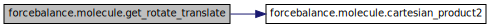
\includegraphics[width=350pt]{namespaceforcebalance_1_1molecule_a08840b73e95bf34bf9ca7ea36ad0492d_cgraph}
\end{center}
\end{figure}


\hypertarget{namespaceforcebalance_1_1molecule_af28de4693e5b8e82df900d0ac3c6c370}{\index{forcebalance\-::molecule@{forcebalance\-::molecule}!get\-Element@{get\-Element}}
\index{get\-Element@{get\-Element}!forcebalance::molecule@{forcebalance\-::molecule}}
\paragraph[{get\-Element}]{\setlength{\rightskip}{0pt plus 5cm}def forcebalance.\-molecule.\-get\-Element (
\begin{DoxyParamCaption}
\item[{}]{mass}
\end{DoxyParamCaption}
)}}\label{namespaceforcebalance_1_1molecule_af28de4693e5b8e82df900d0ac3c6c370}


Definition at line 189 of file molecule.\-py.



Here is the call graph for this function\-:
\nopagebreak
\begin{figure}[H]
\begin{center}
\leavevmode
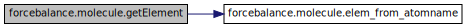
\includegraphics[width=350pt]{namespaceforcebalance_1_1molecule_af28de4693e5b8e82df900d0ac3c6c370_cgraph}
\end{center}
\end{figure}


\hypertarget{namespaceforcebalance_1_1molecule_a7fe52c2928c7b0329882541bef2e34cd}{\index{forcebalance\-::molecule@{forcebalance\-::molecule}!grouper@{grouper}}
\index{grouper@{grouper}!forcebalance::molecule@{forcebalance\-::molecule}}
\paragraph[{grouper}]{\setlength{\rightskip}{0pt plus 5cm}def forcebalance.\-molecule.\-grouper (
\begin{DoxyParamCaption}
\item[{}]{n, }
\item[{}]{iterable}
\end{DoxyParamCaption}
)}}\label{namespaceforcebalance_1_1molecule_a7fe52c2928c7b0329882541bef2e34cd}


Groups a big long iterable into groups of ten or what have you. 



Definition at line 455 of file molecule.\-py.



Here is the call graph for this function\-:
\nopagebreak
\begin{figure}[H]
\begin{center}
\leavevmode
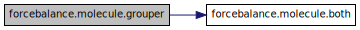
\includegraphics[width=350pt]{namespaceforcebalance_1_1molecule_a7fe52c2928c7b0329882541bef2e34cd_cgraph}
\end{center}
\end{figure}


\hypertarget{namespaceforcebalance_1_1molecule_a838d85848bd817e801d0f5f6502217ef}{\index{forcebalance\-::molecule@{forcebalance\-::molecule}!is\-\_\-charmm\-\_\-coord@{is\-\_\-charmm\-\_\-coord}}
\index{is\-\_\-charmm\-\_\-coord@{is\-\_\-charmm\-\_\-coord}!forcebalance::molecule@{forcebalance\-::molecule}}
\paragraph[{is\-\_\-charmm\-\_\-coord}]{\setlength{\rightskip}{0pt plus 5cm}def forcebalance.\-molecule.\-is\-\_\-charmm\-\_\-coord (
\begin{DoxyParamCaption}
\item[{}]{line}
\end{DoxyParamCaption}
)}}\label{namespaceforcebalance_1_1molecule_a838d85848bd817e801d0f5f6502217ef}


Determines whether a line contains C\-H\-A\-R\-M\-M data or not. 


\begin{DoxyParams}[1]{Parameters}
\mbox{\tt in}  & {\em line} & The line to be tested \\
\hline
\end{DoxyParams}


Definition at line 419 of file molecule.\-py.



Here is the call graph for this function\-:
\nopagebreak
\begin{figure}[H]
\begin{center}
\leavevmode
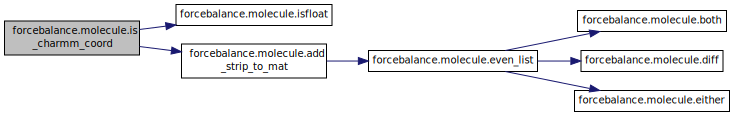
\includegraphics[width=350pt]{namespaceforcebalance_1_1molecule_a838d85848bd817e801d0f5f6502217ef_cgraph}
\end{center}
\end{figure}


\hypertarget{namespaceforcebalance_1_1molecule_aafc8c924eed4480fed8ddc9c474d3bc1}{\index{forcebalance\-::molecule@{forcebalance\-::molecule}!is\-\_\-gro\-\_\-box@{is\-\_\-gro\-\_\-box}}
\index{is\-\_\-gro\-\_\-box@{is\-\_\-gro\-\_\-box}!forcebalance::molecule@{forcebalance\-::molecule}}
\paragraph[{is\-\_\-gro\-\_\-box}]{\setlength{\rightskip}{0pt plus 5cm}def forcebalance.\-molecule.\-is\-\_\-gro\-\_\-box (
\begin{DoxyParamCaption}
\item[{}]{line}
\end{DoxyParamCaption}
)}}\label{namespaceforcebalance_1_1molecule_aafc8c924eed4480fed8ddc9c474d3bc1}


Determines whether a line contains a G\-R\-O\-M\-A\-C\-S box vector or not. 


\begin{DoxyParams}[1]{Parameters}
\mbox{\tt in}  & {\em line} & The line to be tested \\
\hline
\end{DoxyParams}


Definition at line 432 of file molecule.\-py.



Here is the call graph for this function\-:
\nopagebreak
\begin{figure}[H]
\begin{center}
\leavevmode
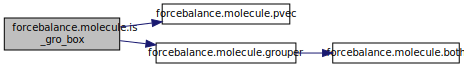
\includegraphics[width=350pt]{namespaceforcebalance_1_1molecule_aafc8c924eed4480fed8ddc9c474d3bc1_cgraph}
\end{center}
\end{figure}


\hypertarget{namespaceforcebalance_1_1molecule_a12b7bb398c2fa49a223f258ec7737483}{\index{forcebalance\-::molecule@{forcebalance\-::molecule}!is\-\_\-gro\-\_\-coord@{is\-\_\-gro\-\_\-coord}}
\index{is\-\_\-gro\-\_\-coord@{is\-\_\-gro\-\_\-coord}!forcebalance::molecule@{forcebalance\-::molecule}}
\paragraph[{is\-\_\-gro\-\_\-coord}]{\setlength{\rightskip}{0pt plus 5cm}def forcebalance.\-molecule.\-is\-\_\-gro\-\_\-coord (
\begin{DoxyParamCaption}
\item[{}]{line}
\end{DoxyParamCaption}
)}}\label{namespaceforcebalance_1_1molecule_a12b7bb398c2fa49a223f258ec7737483}


Determines whether a line contains G\-R\-O\-M\-A\-C\-S data or not. 


\begin{DoxyParams}[1]{Parameters}
\mbox{\tt in}  & {\em line} & The line to be tested \\
\hline
\end{DoxyParams}


Definition at line 404 of file molecule.\-py.



Here is the call graph for this function\-:
\nopagebreak
\begin{figure}[H]
\begin{center}
\leavevmode
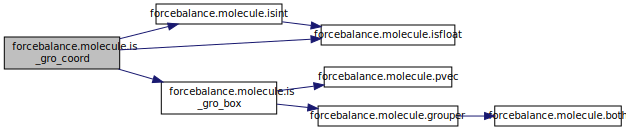
\includegraphics[width=350pt]{namespaceforcebalance_1_1molecule_a12b7bb398c2fa49a223f258ec7737483_cgraph}
\end{center}
\end{figure}


\hypertarget{namespaceforcebalance_1_1molecule_afe989ffd119568047fc8265b1d329a70}{\index{forcebalance\-::molecule@{forcebalance\-::molecule}!isfloat@{isfloat}}
\index{isfloat@{isfloat}!forcebalance::molecule@{forcebalance\-::molecule}}
\paragraph[{isfloat}]{\setlength{\rightskip}{0pt plus 5cm}def forcebalance.\-molecule.\-isfloat (
\begin{DoxyParamCaption}
\item[{}]{word}
\end{DoxyParamCaption}
)}}\label{namespaceforcebalance_1_1molecule_afe989ffd119568047fc8265b1d329a70}


Matches A\-N\-Y number; it can be a decimal, scientific notation, integer, or what have you. 



Definition at line 250 of file molecule.\-py.

\hypertarget{namespaceforcebalance_1_1molecule_a0dd31eff88d2bed0884ab21a13261d42}{\index{forcebalance\-::molecule@{forcebalance\-::molecule}!isint@{isint}}
\index{isint@{isint}!forcebalance::molecule@{forcebalance\-::molecule}}
\paragraph[{isint}]{\setlength{\rightskip}{0pt plus 5cm}def forcebalance.\-molecule.\-isint (
\begin{DoxyParamCaption}
\item[{}]{word}
\end{DoxyParamCaption}
)}}\label{namespaceforcebalance_1_1molecule_a0dd31eff88d2bed0884ab21a13261d42}


O\-N\-L\-Y matches integers! If you have a decimal point? None shall pass! 



Definition at line 245 of file molecule.\-py.



Here is the call graph for this function\-:
\nopagebreak
\begin{figure}[H]
\begin{center}
\leavevmode
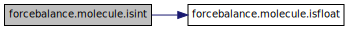
\includegraphics[width=350pt]{namespaceforcebalance_1_1molecule_a0dd31eff88d2bed0884ab21a13261d42_cgraph}
\end{center}
\end{figure}


\hypertarget{namespaceforcebalance_1_1molecule_ab9cb167fbbd809aedcf8c7434d405547}{\index{forcebalance\-::molecule@{forcebalance\-::molecule}!main@{main}}
\index{main@{main}!forcebalance::molecule@{forcebalance\-::molecule}}
\paragraph[{main}]{\setlength{\rightskip}{0pt plus 5cm}def forcebalance.\-molecule.\-main (
\begin{DoxyParamCaption}
{}
\end{DoxyParamCaption}
)}}\label{namespaceforcebalance_1_1molecule_ab9cb167fbbd809aedcf8c7434d405547}


Definition at line 2648 of file molecule.\-py.

\hypertarget{namespaceforcebalance_1_1molecule_ab8464fea13fad2a506792c2f1d7c93f3}{\index{forcebalance\-::molecule@{forcebalance\-::molecule}!nodematch@{nodematch}}
\index{nodematch@{nodematch}!forcebalance::molecule@{forcebalance\-::molecule}}
\paragraph[{nodematch}]{\setlength{\rightskip}{0pt plus 5cm}def forcebalance.\-molecule.\-nodematch (
\begin{DoxyParamCaption}
\item[{}]{node1, }
\item[{}]{node2}
\end{DoxyParamCaption}
)}}\label{namespaceforcebalance_1_1molecule_ab8464fea13fad2a506792c2f1d7c93f3}


Definition at line 239 of file molecule.\-py.



Here is the call graph for this function\-:
\nopagebreak
\begin{figure}[H]
\begin{center}
\leavevmode
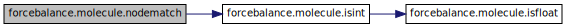
\includegraphics[width=350pt]{namespaceforcebalance_1_1molecule_ab8464fea13fad2a506792c2f1d7c93f3_cgraph}
\end{center}
\end{figure}


\hypertarget{namespaceforcebalance_1_1molecule_a58c3f09152db4d1c6e1db9df29c60c43}{\index{forcebalance\-::molecule@{forcebalance\-::molecule}!pvec@{pvec}}
\index{pvec@{pvec}!forcebalance::molecule@{forcebalance\-::molecule}}
\paragraph[{pvec}]{\setlength{\rightskip}{0pt plus 5cm}def forcebalance.\-molecule.\-pvec (
\begin{DoxyParamCaption}
\item[{}]{vec}
\end{DoxyParamCaption}
)}}\label{namespaceforcebalance_1_1molecule_a58c3f09152db4d1c6e1db9df29c60c43}


Definition at line 450 of file molecule.\-py.



\subsubsection{Variable Documentation}
\hypertarget{namespaceforcebalance_1_1molecule_a2986996d4f957928047df06fbec3717d}{\index{forcebalance\-::molecule@{forcebalance\-::molecule}!Alive@{Alive}}
\index{Alive@{Alive}!forcebalance::molecule@{forcebalance\-::molecule}}
\paragraph[{Alive}]{\setlength{\rightskip}{0pt plus 5cm}forcebalance.\-molecule.\-Alive}}\label{namespaceforcebalance_1_1molecule_a2986996d4f957928047df06fbec3717d}


Definition at line 305 of file molecule.\-py.

\hypertarget{namespaceforcebalance_1_1molecule_a8fcfb88fe12a9256b61980f3d4fe3b63}{\index{forcebalance\-::molecule@{forcebalance\-::molecule}!All\-Variable\-Names@{All\-Variable\-Names}}
\index{All\-Variable\-Names@{All\-Variable\-Names}!forcebalance::molecule@{forcebalance\-::molecule}}
\paragraph[{All\-Variable\-Names}]{\setlength{\rightskip}{0pt plus 5cm}forcebalance.\-molecule.\-All\-Variable\-Names = {\bf Quantum\-Variable\-Names}$|${\bf Atom\-Variable\-Names}$|${\bf Meta\-Variable\-Names}$|${\bf Frame\-Variable\-Names}}}\label{namespaceforcebalance_1_1molecule_a8fcfb88fe12a9256b61980f3d4fe3b63}


Definition at line 137 of file molecule.\-py.

\hypertarget{namespaceforcebalance_1_1molecule_a5daa68e835dcb9877d6c3f2fb559b54b}{\index{forcebalance\-::molecule@{forcebalance\-::molecule}!Atom\-Variable\-Names@{Atom\-Variable\-Names}}
\index{Atom\-Variable\-Names@{Atom\-Variable\-Names}!forcebalance::molecule@{forcebalance\-::molecule}}
\paragraph[{Atom\-Variable\-Names}]{\setlength{\rightskip}{0pt plus 5cm}tuple forcebalance.\-molecule.\-Atom\-Variable\-Names = set(\mbox{[}'elem', 'partial\-\_\-charge', 'atomname', 'atomtype', 'tinkersuf', 'resid', 'resname', 'qcsuf', 'qm\-\_\-ghost', 'chain', 'altloc', 'icode'\mbox{]})}}\label{namespaceforcebalance_1_1molecule_a5daa68e835dcb9877d6c3f2fb559b54b}


Definition at line 120 of file molecule.\-py.

\hypertarget{namespaceforcebalance_1_1molecule_a76af9edfbaaa8999680e32aafe1b1b61}{\index{forcebalance\-::molecule@{forcebalance\-::molecule}!bohrang@{bohrang}}
\index{bohrang@{bohrang}!forcebalance::molecule@{forcebalance\-::molecule}}
\paragraph[{bohrang}]{\setlength{\rightskip}{0pt plus 5cm}float forcebalance.\-molecule.\-bohrang = 0.\-529177249}}\label{namespaceforcebalance_1_1molecule_a76af9edfbaaa8999680e32aafe1b1b61}


One bohr equals this many angstroms. 



Definition at line 237 of file molecule.\-py.

\hypertarget{namespaceforcebalance_1_1molecule_aa761cf1cf260e15d0b03a6f61569c840}{\index{forcebalance\-::molecule@{forcebalance\-::molecule}!Box@{Box}}
\index{Box@{Box}!forcebalance::molecule@{forcebalance\-::molecule}}
\paragraph[{Box}]{\setlength{\rightskip}{0pt plus 5cm}tuple forcebalance.\-molecule.\-Box = namedtuple('Box',\mbox{[}'a','b','c','alpha','beta','gamma','A','B','C','V'\mbox{]})}}\label{namespaceforcebalance_1_1molecule_aa761cf1cf260e15d0b03a6f61569c840}


Definition at line 257 of file molecule.\-py.

\hypertarget{namespaceforcebalance_1_1molecule_a1c99a11e8a749468698c9af6361a8a4c}{\index{forcebalance\-::molecule@{forcebalance\-::molecule}!Elements@{Elements}}
\index{Elements@{Elements}!forcebalance::molecule@{forcebalance\-::molecule}}
\paragraph[{Elements}]{\setlength{\rightskip}{0pt plus 5cm}list forcebalance.\-molecule.\-Elements}}\label{namespaceforcebalance_1_1molecule_a1c99a11e8a749468698c9af6361a8a4c}
{\bfseries Initial value\-:}
\begin{DoxyCode}
1 = [\textcolor{stringliteral}{"None"},\textcolor{stringliteral}{'H'},\textcolor{stringliteral}{'He'},
2             \textcolor{stringliteral}{'Li'},\textcolor{stringliteral}{'Be'},\textcolor{stringliteral}{'B'},\textcolor{stringliteral}{'C'},\textcolor{stringliteral}{'N'},\textcolor{stringliteral}{'O'},\textcolor{stringliteral}{'F'},\textcolor{stringliteral}{'Ne'},
3             \textcolor{stringliteral}{'Na'},\textcolor{stringliteral}{'Mg'},\textcolor{stringliteral}{'Al'},\textcolor{stringliteral}{'Si'},\textcolor{stringliteral}{'P'},\textcolor{stringliteral}{'S'},\textcolor{stringliteral}{'Cl'},\textcolor{stringliteral}{'Ar'},
4             \textcolor{stringliteral}{'K'},\textcolor{stringliteral}{'Ca'},\textcolor{stringliteral}{'Sc'},\textcolor{stringliteral}{'Ti'},\textcolor{stringliteral}{'V'},\textcolor{stringliteral}{'Cr'},\textcolor{stringliteral}{'Mn'},\textcolor{stringliteral}{'Fe'},\textcolor{stringliteral}{'Co'},\textcolor{stringliteral}{'Ni'},\textcolor{stringliteral}{'Cu'},\textcolor{stringliteral}{'Zn'},\textcolor{stringliteral}{'Ga'},\textcolor{stringliteral}{'Ge'},\textcolor{stringliteral}{'As'},\textcolor{stringliteral}{'Se'},\textcolor{stringliteral}{'Br'},\textcolor{stringliteral}{'Kr'},
5             \textcolor{stringliteral}{'Rb'},\textcolor{stringliteral}{'Sr'},\textcolor{stringliteral}{'Y'},\textcolor{stringliteral}{'Zr'},\textcolor{stringliteral}{'Nb'},\textcolor{stringliteral}{'Mo'},\textcolor{stringliteral}{'Tc'},\textcolor{stringliteral}{'Ru'},\textcolor{stringliteral}{'Rh'},\textcolor{stringliteral}{'Pd'},\textcolor{stringliteral}{'Ag'},\textcolor{stringliteral}{'Cd'},\textcolor{stringliteral}{'In'},\textcolor{stringliteral}{'Sn'},\textcolor{stringliteral}{'Sb'},\textcolor{stringliteral}{'Te'},\textcolor{stringliteral}{'I'},\textcolor{stringliteral}{'Xe'},
6             \textcolor{stringliteral}{'Cs'},\textcolor{stringliteral}{'Ba'},\textcolor{stringliteral}{'La'},\textcolor{stringliteral}{'Ce'},\textcolor{stringliteral}{'Pr'},\textcolor{stringliteral}{'Nd'},\textcolor{stringliteral}{'Pm'},\textcolor{stringliteral}{'Sm'},\textcolor{stringliteral}{'Eu'},\textcolor{stringliteral}{'Gd'},\textcolor{stringliteral}{'Tb'},\textcolor{stringliteral}{'Dy'},\textcolor{stringliteral}{'Ho'},\textcolor{stringliteral}{'Er'},\textcolor{stringliteral}{'Tm'},\textcolor{stringliteral}{'Yb'},
7             \textcolor{stringliteral}{'Lu'},\textcolor{stringliteral}{'Hf'},\textcolor{stringliteral}{'Ta'},\textcolor{stringliteral}{'W'},\textcolor{stringliteral}{'Re'},\textcolor{stringliteral}{'Os'},\textcolor{stringliteral}{'Ir'},\textcolor{stringliteral}{'Pt'},\textcolor{stringliteral}{'Au'},\textcolor{stringliteral}{'Hg'},\textcolor{stringliteral}{'Tl'},\textcolor{stringliteral}{'Pb'},\textcolor{stringliteral}{'Bi'},\textcolor{stringliteral}{'Po'},\textcolor{stringliteral}{'At'},\textcolor{stringliteral}{'Rn'},
8             \textcolor{stringliteral}{'Fr'},\textcolor{stringliteral}{'Ra'},\textcolor{stringliteral}{'Ac'},\textcolor{stringliteral}{'Th'},\textcolor{stringliteral}{'Pa'},\textcolor{stringliteral}{'}\textcolor{stringliteral}{U','}Np','Pu','Am','Cm','Bk','Cf','Es','Fm','Md','No','Lr','Rf','Db','
      Sg','Bh','Hs','Mt']
\end{DoxyCode}


Definition at line 164 of file molecule.\-py.

\hypertarget{namespaceforcebalance_1_1molecule_a0044fa397e0923635a8b3e9625aa70f7}{\index{forcebalance\-::molecule@{forcebalance\-::molecule}!Frame\-Variable\-Names@{Frame\-Variable\-Names}}
\index{Frame\-Variable\-Names@{Frame\-Variable\-Names}!forcebalance::molecule@{forcebalance\-::molecule}}
\paragraph[{Frame\-Variable\-Names}]{\setlength{\rightskip}{0pt plus 5cm}tuple forcebalance.\-molecule.\-Frame\-Variable\-Names}}\label{namespaceforcebalance_1_1molecule_a0044fa397e0923635a8b3e9625aa70f7}
{\bfseries Initial value\-:}
\begin{DoxyCode}
1 = set([\textcolor{stringliteral}{'xyzs'}, \textcolor{stringliteral}{'comms'}, \textcolor{stringliteral}{'boxes'}, \textcolor{stringliteral}{'qm\_forces'}, \textcolor{stringliteral}{'qm\_energies'}, \textcolor{stringliteral}{'qm\_interaction'}, 
2                           \textcolor{stringliteral}{'qm\_espxyzs'}, \textcolor{stringliteral}{'qm\_espvals'}, \textcolor{stringliteral}{'qm\_extchgs'}, \textcolor{stringliteral}{'qm\_mulliken\_charges'}, \textcolor{stringliteral}{'
      qm\_mulliken\_spins'}])
\end{DoxyCode}


Definition at line 106 of file molecule.\-py.

\hypertarget{namespaceforcebalance_1_1molecule_a38e1c99e9567fe42b792af43db9b7488}{\index{forcebalance\-::molecule@{forcebalance\-::molecule}!Meta\-Variable\-Names@{Meta\-Variable\-Names}}
\index{Meta\-Variable\-Names@{Meta\-Variable\-Names}!forcebalance::molecule@{forcebalance\-::molecule}}
\paragraph[{Meta\-Variable\-Names}]{\setlength{\rightskip}{0pt plus 5cm}tuple forcebalance.\-molecule.\-Meta\-Variable\-Names = set(\mbox{[}'fnm', 'ftype', 'qcrems', 'qctemplate', 'charge', 'mult', 'bonds'\mbox{]})}}\label{namespaceforcebalance_1_1molecule_a38e1c99e9567fe42b792af43db9b7488}


Definition at line 133 of file molecule.\-py.

\hypertarget{namespaceforcebalance_1_1molecule_adc5040ec456762f2ac240fb08febbfdd}{\index{forcebalance\-::molecule@{forcebalance\-::molecule}!Periodic\-Table@{Periodic\-Table}}
\index{Periodic\-Table@{Periodic\-Table}!forcebalance::molecule@{forcebalance\-::molecule}}
\paragraph[{Periodic\-Table}]{\setlength{\rightskip}{0pt plus 5cm}tuple forcebalance.\-molecule.\-Periodic\-Table}}\label{namespaceforcebalance_1_1molecule_adc5040ec456762f2ac240fb08febbfdd}
{\bfseries Initial value\-:}
\begin{DoxyCode}
1 = OrderedDict([(\textcolor{stringliteral}{'H'} , 1.0079), (\textcolor{stringliteral}{'He'} , 4.0026), 
2                              (\textcolor{stringliteral}{'Li'} , 6.941), (\textcolor{stringliteral}{'Be'} , 9.0122), (\textcolor{stringliteral}{'B'} , 10.811), (\textcolor{stringliteral}{'C'} , 12.0107), (\textcolor{stringliteral}{'N'} , 14.00
      67), (\textcolor{stringliteral}{'O'} , 15.9994), (\textcolor{stringliteral}{'F'} , 18.9984), (\textcolor{stringliteral}{'Ne'} , 20.1797),
3                              (\textcolor{stringliteral}{'Na'} , 22.9897), (\textcolor{stringliteral}{'Mg'} , 24.305), (\textcolor{stringliteral}{'Al'} , 26.9815), (\textcolor{stringliteral}{'Si'} , 28.0855), (\textcolor{stringliteral}{'P'} , 
      30.9738), (\textcolor{stringliteral}{'S'} , 32.065), (\textcolor{stringliteral}{'Cl'} , 35.453), (\textcolor{stringliteral}{'Ar'} , 39.948), 
4                              (\textcolor{stringliteral}{'K'} , 39.0983), (\textcolor{stringliteral}{'Ca'} , 40.078), (\textcolor{stringliteral}{'Sc'} , 44.9559), (\textcolor{stringliteral}{'Ti'} , 47.867), (\textcolor{stringliteral}{'V'} , 50
      .9415), (\textcolor{stringliteral}{'Cr'} , 51.9961), (\textcolor{stringliteral}{'Mn'} , 54.938), (\textcolor{stringliteral}{'Fe'} , 55.845), (\textcolor{stringliteral}{'Co'} , 58.9332), 
5                              (\textcolor{stringliteral}{'Ni'} , 58.6934), (\textcolor{stringliteral}{'Cu'} , 63.546), (\textcolor{stringliteral}{'Zn'} , 65.39), (\textcolor{stringliteral}{'Ga'} , 69.723), (\textcolor{stringliteral}{'Ge'} , 72
      .64), (\textcolor{stringliteral}{'As'} , 74.9216), (\textcolor{stringliteral}{'Se'} , 78.96), (\textcolor{stringliteral}{'Br'} , 79.904), (\textcolor{stringliteral}{'Kr'} , 83.8), 
6                              (\textcolor{stringliteral}{'Rb'} , 85.4678), (\textcolor{stringliteral}{'Sr'} , 87.62), (\textcolor{stringliteral}{'Y'} , 88.9059), (\textcolor{stringliteral}{'Zr'} , 91.224), (\textcolor{stringliteral}{'Nb'} , 92
      .9064), (\textcolor{stringliteral}{'Mo'} , 95.94), (\textcolor{stringliteral}{'Tc'} , 98), (\textcolor{stringliteral}{'Ru'} , 101.07), (\textcolor{stringliteral}{'Rh'} , 102.9055), 
7                              (\textcolor{stringliteral}{'Pd'} , 106.42), (\textcolor{stringliteral}{'Ag'} , 107.8682), (\textcolor{stringliteral}{'Cd'} , 112.411), (\textcolor{stringliteral}{'In'} , 114.818), (\textcolor{stringliteral}{'Sn'} 
      , 118.71), (\textcolor{stringliteral}{'Sb'} , 121.76), (\textcolor{stringliteral}{'Te'} , 127.6), (\textcolor{stringliteral}{'I'} , 126.9045), (\textcolor{stringliteral}{'Xe'} , 131.293), 
8                              (\textcolor{stringliteral}{'Cs'} , 132.9055), (\textcolor{stringliteral}{'Ba'} , 137.327), (\textcolor{stringliteral}{'La'} , 138.9055), (\textcolor{stringliteral}{'Ce'} , 140.116), (\textcolor{stringliteral}{'Pr
      '} , 140.9077), (\textcolor{stringliteral}{'Nd'} , 144.24), (\textcolor{stringliteral}{'Pm'} , 145), (\textcolor{stringliteral}{'Sm'} , 150.36), 
9                              (\textcolor{stringliteral}{'Eu'} , 151.964), (\textcolor{stringliteral}{'Gd'} , 157.25), (\textcolor{stringliteral}{'Tb'} , 158.9253), (\textcolor{stringliteral}{'Dy'} , 162.5), (\textcolor{stringliteral}{'Ho'} , 
      164.9303), (\textcolor{stringliteral}{'Er'} , 167.259), (\textcolor{stringliteral}{'Tm'} , 168.9342), (\textcolor{stringliteral}{'Yb'} , 173.04), 
10                              (\textcolor{stringliteral}{'Lu'} , 174.967), (\textcolor{stringliteral}{'Hf'} , 178.49), (\textcolor{stringliteral}{'Ta'} , 180.9479), (\textcolor{stringliteral}{'W'} , 183.84), (\textcolor{stringliteral}{'Re'} , 
      186.207), (\textcolor{stringliteral}{'Os'} , 190.23), (\textcolor{stringliteral}{'Ir'} , 192.217), (\textcolor{stringliteral}{'Pt'} , 195.078), 
11                              (\textcolor{stringliteral}{'Au'} , 196.9665), (\textcolor{stringliteral}{'Hg'} , 200.59), (\textcolor{stringliteral}{'Tl'} , 204.3833), (\textcolor{stringliteral}{'Pb'} , 207.2), (\textcolor{stringliteral}{'Bi'} ,
       208.9804), (\textcolor{stringliteral}{'Po'} , 209), (\textcolor{stringliteral}{'At'} , 210), (\textcolor{stringliteral}{'Rn'} , 222), 
12                              (\textcolor{stringliteral}{'Fr'} , 223), (\textcolor{stringliteral}{'Ra'} , 226), (\textcolor{stringliteral}{'Ac'} , 227), (\textcolor{stringliteral}{'Th'} , 232.0381), (\textcolor{stringliteral}{'Pa'} , 231.0359)
      , (\textcolor{stringliteral}{'}\textcolor{stringliteral}{U' , 238.0289), ('}Np' , 237), ('Pu' , 244), 
13                              (\textcolor{stringliteral}{'Am'} , 243), (\textcolor{stringliteral}{'Cm'} , 247), (\textcolor{stringliteral}{'Bk'} , 247), (\textcolor{stringliteral}{'Cf'} , 251), (\textcolor{stringliteral}{'Es'} , 252), (\textcolor{stringliteral}{'Fm'} , 
      257), (\textcolor{stringliteral}{'Md'} , 258), (\textcolor{stringliteral}{'No'} , 259), 
14                              (\textcolor{stringliteral}{'Lr'} , 262), (\textcolor{stringliteral}{'Rf'} , 261), (\textcolor{stringliteral}{'Db'} , 262), (\textcolor{stringliteral}{'Sg'} , 266), (\textcolor{stringliteral}{'Bh'} , 264), (\textcolor{stringliteral}{'Hs'} , 
      277), (\textcolor{stringliteral}{'Mt'} , 268)])
\end{DoxyCode}


Definition at line 174 of file molecule.\-py.

\hypertarget{namespaceforcebalance_1_1molecule_ab67efeab6049ec1f416b9ad1eed6ffcc}{\index{forcebalance\-::molecule@{forcebalance\-::molecule}!Quantum\-Variable\-Names@{Quantum\-Variable\-Names}}
\index{Quantum\-Variable\-Names@{Quantum\-Variable\-Names}!forcebalance::molecule@{forcebalance\-::molecule}}
\paragraph[{Quantum\-Variable\-Names}]{\setlength{\rightskip}{0pt plus 5cm}tuple forcebalance.\-molecule.\-Quantum\-Variable\-Names = set(\mbox{[}'qcrems', 'qctemplate', 'charge', 'mult', 'qcsuf', 'qm\-\_\-ghost'\mbox{]})}}\label{namespaceforcebalance_1_1molecule_ab67efeab6049ec1f416b9ad1eed6ffcc}


Definition at line 135 of file molecule.\-py.

\hypertarget{namespaceforcebalance_1_1molecule_a1ee5389ce8a9042e053c7972dbbfb005}{\index{forcebalance\-::molecule@{forcebalance\-::molecule}!radian@{radian}}
\index{radian@{radian}!forcebalance::molecule@{forcebalance\-::molecule}}
\paragraph[{radian}]{\setlength{\rightskip}{0pt plus 5cm}int forcebalance.\-molecule.\-radian = 180}}\label{namespaceforcebalance_1_1molecule_a1ee5389ce8a9042e053c7972dbbfb005}


Definition at line 258 of file molecule.\-py.

\hypertarget{namespaceforcebalance_1_1molecule_a74f55a89a14ca676b5a06441d1fdab19}{\index{forcebalance\-::molecule@{forcebalance\-::molecule}!Radii@{Radii}}
\index{Radii@{Radii}!forcebalance::molecule@{forcebalance\-::molecule}}
\paragraph[{Radii}]{\setlength{\rightskip}{0pt plus 5cm}list forcebalance.\-molecule.\-Radii}}\label{namespaceforcebalance_1_1molecule_a74f55a89a14ca676b5a06441d1fdab19}
{\bfseries Initial value\-:}
\begin{DoxyCode}
1 = [0.31, 0.28, \textcolor{comment}{# H and He}
2          1.28, 0.96, 0.84, 0.76, 0.71, 0.66, 0.57, 0.58, \textcolor{comment}{# First row elements}
3          1.66, 1.41, 1.21, 1.11, 1.07, 1.05, 1.02, 1.06, \textcolor{comment}{# Second row elements}
4          2.03, 1.76, 1.70, 1.60, 1.53, 1.39, 1.61, 1.52, 1.50, 
5          1.24, 1.32, 1.22, 1.22, 1.20, 1.19, 1.20, 1.20, 1.16, \textcolor{comment}{# Third row elements, K through Kr}
6          2.20, 1.95, 1.90, 1.75, 1.64, 1.54, 1.47, 1.46, 1.42, 
7          1.39, 1.45, 1.44, 1.42, 1.39, 1.39, 1.38, 1.39, 1.40, \textcolor{comment}{# Fourth row elements, Rb through Xe}
8          2.44, 2.15, 2.07, 2.04, 2.03, 2.01, 1.99, 1.98, 
9          1.98, 1.96, 1.94, 1.92, 1.92, 1.89, 1.90, 1.87, \textcolor{comment}{# Fifth row elements, s and f blocks}
10          1.87, 1.75, 1.70, 1.62, 1.51, 1.44, 1.41, 1.36, 
11          1.36, 1.32, 1.45, 1.46, 1.48, 1.40, 1.50, 1.50, \textcolor{comment}{# Fifth row elements, d and p blocks}
12          2.60, 2.21, 2.15, 2.06, 2.00, 1.96, 1.90, 1.87, 1.80, 1.69]
\end{DoxyCode}


Definition at line 150 of file molecule.\-py.

\hypertarget{namespaceforcebalance_1_1molecule_a09d04113accea9c88b084051c5de29d1}{\index{forcebalance\-::molecule@{forcebalance\-::molecule}!splitter@{splitter}}
\index{splitter@{splitter}!forcebalance::molecule@{forcebalance\-::molecule}}
\paragraph[{splitter}]{\setlength{\rightskip}{0pt plus 5cm}tuple forcebalance.\-molecule.\-splitter = re.\-compile(r'(\textbackslash{}s+$|$\textbackslash{}S+)')}}\label{namespaceforcebalance_1_1molecule_a09d04113accea9c88b084051c5de29d1}


Definition at line 254 of file molecule.\-py.


\hypertarget{namespaceforcebalance_1_1moments}{\subsection{forcebalance\-:\-:moments \-Namespace \-Reference}
\label{namespaceforcebalance_1_1moments}\index{forcebalance\-::moments@{forcebalance\-::moments}}
}


\-Multipole moment fitting module.  


\subsubsection*{\-Classes}
\begin{DoxyCompactItemize}
\item 
class \hyperlink{classforcebalance_1_1moments_1_1Moments}{\-Moments}
\begin{DoxyCompactList}\small\item\em \-Subclass of \-Target for fitting force fields to multipole moments (from experiment or theory). \end{DoxyCompactList}\end{DoxyCompactItemize}
\subsubsection*{\-Variables}
\begin{DoxyCompactItemize}
\item 
tuple \hyperlink{namespaceforcebalance_1_1moments_a92133a6e6d1078c3f8986326bd63e184}{logger} = get\-Logger(\-\_\-\-\_\-name\-\_\-\-\_\-)
\end{DoxyCompactItemize}


\subsubsection{\-Detailed \-Description}
\-Multipole moment fitting module. \begin{DoxyAuthor}{\-Author}
\-Lee-\/\-Ping \-Wang 
\end{DoxyAuthor}
\begin{DoxyDate}{\-Date}
09/2012 
\end{DoxyDate}


\subsubsection{\-Variable \-Documentation}
\hypertarget{namespaceforcebalance_1_1moments_a92133a6e6d1078c3f8986326bd63e184}{\index{forcebalance\-::moments@{forcebalance\-::moments}!logger@{logger}}
\index{logger@{logger}!forcebalance::moments@{forcebalance\-::moments}}
\paragraph[{logger}]{\setlength{\rightskip}{0pt plus 5cm}tuple {\bf forcebalance\-::moments\-::logger} = get\-Logger(\-\_\-\-\_\-name\-\_\-\-\_\-)}}\label{namespaceforcebalance_1_1moments_a92133a6e6d1078c3f8986326bd63e184}


\-Definition at line 22 of file moments.\-py.


\hypertarget{namespaceforcebalance_1_1nifty}{\subsection{forcebalance.\-nifty Namespace Reference}
\label{namespaceforcebalance_1_1nifty}\index{forcebalance.\-nifty@{forcebalance.\-nifty}}
}

\hypertarget{namespaceforcebalance_1_1objective}{\subsection{forcebalance.\-objective Namespace Reference}
\label{namespaceforcebalance_1_1objective}\index{forcebalance.\-objective@{forcebalance.\-objective}}
}


Force\-Balance objective function.  


\subsubsection*{Classes}
\begin{DoxyCompactItemize}
\item 
class \hyperlink{classforcebalance_1_1objective_1_1Objective}{Objective}
\begin{DoxyCompactList}\small\item\em \hyperlink{classforcebalance_1_1objective_1_1Objective}{Objective} function. \end{DoxyCompactList}\item 
class \hyperlink{classforcebalance_1_1objective_1_1Penalty}{Penalty}
\begin{DoxyCompactList}\small\item\em \hyperlink{classforcebalance_1_1objective_1_1Penalty}{Penalty} functions for regularizing the force field optimizer. \end{DoxyCompactList}\end{DoxyCompactItemize}
\subsubsection*{Variables}
\begin{DoxyCompactItemize}
\item 
tuple \hyperlink{namespaceforcebalance_1_1objective_ac2e1e8c9612652836168e5cdde77b6e7}{logger} = get\-Logger(\-\_\-\-\_\-name\-\_\-\-\_\-)
\item 
dictionary \hyperlink{namespaceforcebalance_1_1objective_a8c93e21f995ed17addb493ec94368ab5}{Implemented\-\_\-\-Targets}
\begin{DoxyCompactList}\small\item\em The table of implemented Targets. \end{DoxyCompactList}\item 
list \hyperlink{namespaceforcebalance_1_1objective_a89a971322532b36852765b2680651f1f}{Letters} = \mbox{[}'X','G','H'\mbox{]}
\begin{DoxyCompactList}\small\item\em This is the canonical lettering that corresponds to \-: objective function, gradient, Hessian. \end{DoxyCompactList}\end{DoxyCompactItemize}


\subsubsection{Detailed Description}
Force\-Balance objective function. 

\subsubsection{Variable Documentation}
\hypertarget{namespaceforcebalance_1_1objective_a8c93e21f995ed17addb493ec94368ab5}{\index{forcebalance\-::objective@{forcebalance\-::objective}!Implemented\-\_\-\-Targets@{Implemented\-\_\-\-Targets}}
\index{Implemented\-\_\-\-Targets@{Implemented\-\_\-\-Targets}!forcebalance::objective@{forcebalance\-::objective}}
\paragraph[{Implemented\-\_\-\-Targets}]{\setlength{\rightskip}{0pt plus 5cm}dictionary forcebalance.\-objective.\-Implemented\-\_\-\-Targets}}\label{namespaceforcebalance_1_1objective_a8c93e21f995ed17addb493ec94368ab5}
{\bfseries Initial value\-:}
\begin{DoxyCode}
1 = \{
2     \textcolor{stringliteral}{'ABINITIO\_GMX'}:AbInitio\_GMX,
3     \textcolor{stringliteral}{'ABINITIO\_TINKER'}:AbInitio\_TINKER,
4     \textcolor{stringliteral}{'ABINITIO\_OPENMM'}:AbInitio\_OpenMM,
5     \textcolor{stringliteral}{'ABINITIO\_AMBER'}:AbInitio\_AMBER,
6     \textcolor{stringliteral}{'ABINITIO\_INTERNAL'}:AbInitio\_Internal,
7     \textcolor{stringliteral}{'VIBRATION\_TINKER'}:Vibration\_TINKER,
8     \textcolor{stringliteral}{'VIBRATION\_GMX'}:Vibration\_GMX,
9     \textcolor{stringliteral}{'THERMO\_GMX'}:Thermo\_GMX,
10     \textcolor{stringliteral}{'LIQUID\_OPENMM'}:Liquid\_OpenMM,
11     \textcolor{stringliteral}{'LIQUID\_TINKER'}:Liquid\_TINKER, 
12     \textcolor{stringliteral}{'LIQUID\_GMX'}:Liquid\_GMX, 
13     \textcolor{stringliteral}{'LIPID\_GMX'}:Lipid\_GMX, 
14     \textcolor{stringliteral}{'COUNTERPOISE'}:Counterpoise,
15     \textcolor{stringliteral}{'THCDF\_PSI4'}:THCDF\_Psi4,
16     \textcolor{stringliteral}{'RDVR3\_PSI4'}:RDVR3\_Psi4,
17     \textcolor{stringliteral}{'INTERACTION\_GMX'}:Interaction\_GMX,
18     \textcolor{stringliteral}{'INTERACTION\_TINKER'}:Interaction\_TINKER,
19     \textcolor{stringliteral}{'INTERACTION\_OPENMM'}:Interaction\_OpenMM,
20     \textcolor{stringliteral}{'BINDINGENERGY\_TINKER'}:BindingEnergy\_TINKER,
21     \textcolor{stringliteral}{'BINDINGENERGY\_GMX'}:BindingEnergy\_GMX,
22     \textcolor{stringliteral}{'BINDINGENERGY\_OPENMM'}:BindingEnergy\_OpenMM,
23     \textcolor{stringliteral}{'MOMENTS\_TINKER'}:Moments\_TINKER,
24     \textcolor{stringliteral}{'MOMENTS\_GMX'}:Moments\_GMX,
25     \textcolor{stringliteral}{'MOMENTS\_OPENMM'}:Moments\_OpenMM,
26     \textcolor{stringliteral}{'REMOTE\_TARGET'}:RemoteTarget,
27     \}
\end{DoxyCode}


The table of implemented Targets. 



Definition at line 68 of file objective.\-py.

\hypertarget{namespaceforcebalance_1_1objective_a89a971322532b36852765b2680651f1f}{\index{forcebalance\-::objective@{forcebalance\-::objective}!Letters@{Letters}}
\index{Letters@{Letters}!forcebalance::objective@{forcebalance\-::objective}}
\paragraph[{Letters}]{\setlength{\rightskip}{0pt plus 5cm}list forcebalance.\-objective.\-Letters = \mbox{[}'X','G','H'\mbox{]}}}\label{namespaceforcebalance_1_1objective_a89a971322532b36852765b2680651f1f}


This is the canonical lettering that corresponds to \-: objective function, gradient, Hessian. 



Definition at line 97 of file objective.\-py.

\hypertarget{namespaceforcebalance_1_1objective_ac2e1e8c9612652836168e5cdde77b6e7}{\index{forcebalance\-::objective@{forcebalance\-::objective}!logger@{logger}}
\index{logger@{logger}!forcebalance::objective@{forcebalance\-::objective}}
\paragraph[{logger}]{\setlength{\rightskip}{0pt plus 5cm}tuple forcebalance.\-objective.\-logger = get\-Logger(\-\_\-\-\_\-name\-\_\-\-\_\-)}}\label{namespaceforcebalance_1_1objective_ac2e1e8c9612652836168e5cdde77b6e7}


Definition at line 17 of file objective.\-py.


\hypertarget{namespaceforcebalance_1_1openmmio}{\subsection{forcebalance.\-openmmio Namespace Reference}
\label{namespaceforcebalance_1_1openmmio}\index{forcebalance.\-openmmio@{forcebalance.\-openmmio}}
}


\hyperlink{classforcebalance_1_1openmmio_1_1OpenMM}{Open\-M\-M} input/output.  


\subsubsection*{Classes}
\begin{DoxyCompactItemize}
\item 
class \hyperlink{classforcebalance_1_1openmmio_1_1OpenMM__Reader}{Open\-M\-M\-\_\-\-Reader}
\begin{DoxyCompactList}\small\item\em Class for parsing \hyperlink{classforcebalance_1_1openmmio_1_1OpenMM}{Open\-M\-M} force field files. \end{DoxyCompactList}\item 
class \hyperlink{classforcebalance_1_1openmmio_1_1OpenMM}{Open\-M\-M}
\begin{DoxyCompactList}\small\item\em Derived from Engine object for carrying out general purpose \hyperlink{classforcebalance_1_1openmmio_1_1OpenMM}{Open\-M\-M} calculations. \end{DoxyCompactList}\item 
class \hyperlink{classforcebalance_1_1openmmio_1_1Liquid__OpenMM}{Liquid\-\_\-\-Open\-M\-M}
\begin{DoxyCompactList}\small\item\em Condensed phase property matching using \hyperlink{classforcebalance_1_1openmmio_1_1OpenMM}{Open\-M\-M}. \end{DoxyCompactList}\item 
class \hyperlink{classforcebalance_1_1openmmio_1_1AbInitio__OpenMM}{Ab\-Initio\-\_\-\-Open\-M\-M}
\begin{DoxyCompactList}\small\item\em Force and energy matching using \hyperlink{classforcebalance_1_1openmmio_1_1OpenMM}{Open\-M\-M}. \end{DoxyCompactList}\item 
class \hyperlink{classforcebalance_1_1openmmio_1_1BindingEnergy__OpenMM}{Binding\-Energy\-\_\-\-Open\-M\-M}
\begin{DoxyCompactList}\small\item\em Binding energy matching using \hyperlink{classforcebalance_1_1openmmio_1_1OpenMM}{Open\-M\-M}. \end{DoxyCompactList}\item 
class \hyperlink{classforcebalance_1_1openmmio_1_1Interaction__OpenMM}{Interaction\-\_\-\-Open\-M\-M}
\begin{DoxyCompactList}\small\item\em Interaction matching using \hyperlink{classforcebalance_1_1openmmio_1_1OpenMM}{Open\-M\-M}. \end{DoxyCompactList}\item 
class \hyperlink{classforcebalance_1_1openmmio_1_1Moments__OpenMM}{Moments\-\_\-\-Open\-M\-M}
\begin{DoxyCompactList}\small\item\em Multipole moment matching using \hyperlink{classforcebalance_1_1openmmio_1_1OpenMM}{Open\-M\-M}. \end{DoxyCompactList}\end{DoxyCompactItemize}
\subsubsection*{Functions}
\begin{DoxyCompactItemize}
\item 
def \hyperlink{namespaceforcebalance_1_1openmmio_a0266102cb0a6907750a62e6948299255}{energy\-\_\-components}
\item 
def \hyperlink{namespaceforcebalance_1_1openmmio_a829487387c4b4a4817a2e3fc50242857}{get\-\_\-multipoles}
\begin{DoxyCompactList}\small\item\em Return the current multipole moments in Debye and Buckingham units. \end{DoxyCompactList}\item 
def \hyperlink{namespaceforcebalance_1_1openmmio_a8a2081dcaf027b9b9ab224e22680714d}{get\-\_\-dipole}
\begin{DoxyCompactList}\small\item\em Return the current dipole moment in Debye. \end{DoxyCompactList}\item 
def \hyperlink{namespaceforcebalance_1_1openmmio_ac7c1f986acada081a7c24a5d77701a35}{Prepare\-Virtual\-Sites}
\begin{DoxyCompactList}\small\item\em Prepare a list of function wrappers and vsite parameters from the system. \end{DoxyCompactList}\item 
def \hyperlink{namespaceforcebalance_1_1openmmio_a1f92d88085657ca5726f8925bfa68f6f}{Reset\-Virtual\-Sites\-\_\-fast}
\begin{DoxyCompactList}\small\item\em Given a set of Open\-M\-M-\/compatible positions and a System object, compute the correct virtual site positions according to the System. \end{DoxyCompactList}\item 
def \hyperlink{namespaceforcebalance_1_1openmmio_af623fa5af97de6c6a0bc5f98ce8db432}{Reset\-Virtual\-Sites}
\begin{DoxyCompactList}\small\item\em Given a set of Open\-M\-M-\/compatible positions and a System object, compute the correct virtual site positions according to the System. \end{DoxyCompactList}\item 
def \hyperlink{namespaceforcebalance_1_1openmmio_a71e9c5b9d6a71839f5e04cd7ad7351db}{Get\-Virtual\-Site\-Parameters}
\begin{DoxyCompactList}\small\item\em Return an array of all virtual site parameters in the system. \end{DoxyCompactList}\item 
def \hyperlink{namespaceforcebalance_1_1openmmio_a792a195b31612f2140b35927fe28fa1a}{Copy\-Amoeba\-Bond\-Parameters}
\item 
def \hyperlink{namespaceforcebalance_1_1openmmio_a2e95f600757655d41660c25af8fd8e80}{Copy\-Amoeba\-Out\-Of\-Plane\-Bend\-Parameters}
\item 
def \hyperlink{namespaceforcebalance_1_1openmmio_abe9a6b9b200dc8487e56dad7249af3ec}{Copy\-Amoeba\-Angle\-Parameters}
\item 
def \hyperlink{namespaceforcebalance_1_1openmmio_ad0d4739f80f2aab1a861f2e03b8efcd6}{Copy\-Amoeba\-In\-Plane\-Angle\-Parameters}
\item 
def \hyperlink{namespaceforcebalance_1_1openmmio_abe005f73c6dfe9ce1052c9434bcad9be}{Copy\-Amoeba\-Vdw\-Parameters}
\item 
def \hyperlink{namespaceforcebalance_1_1openmmio_a3706c19e71969cabe5782a4535abeffe}{Copy\-Amoeba\-Multipole\-Parameters}
\item 
def \hyperlink{namespaceforcebalance_1_1openmmio_a616f12cc53381716e5fa41f00bf623be}{Copy\-Harmonic\-Bond\-Parameters}
\item 
def \hyperlink{namespaceforcebalance_1_1openmmio_af4ed16f5e2b1cd12bce2f25fab1b05bc}{Copy\-Harmonic\-Angle\-Parameters}
\item 
def \hyperlink{namespaceforcebalance_1_1openmmio_a8f13702754f0b4e43e272139a2ce8341}{Copy\-Periodic\-Torsion\-Parameters}
\item 
def \hyperlink{namespaceforcebalance_1_1openmmio_afead47464a644d9225f9fa8eb568a8ed}{Copy\-Nonbonded\-Parameters}
\item 
def \hyperlink{namespaceforcebalance_1_1openmmio_a2bb7add6b813d94f2655372c51fe8fdc}{do\-\_\-nothing}
\item 
def \hyperlink{namespaceforcebalance_1_1openmmio_a8c6ed589ec2b35b8363a529ffdf88eb0}{Copy\-System\-Parameters}
\begin{DoxyCompactList}\small\item\em Copy parameters from one system (i.\-e. \end{DoxyCompactList}\item 
def \hyperlink{namespaceforcebalance_1_1openmmio_a9f9fc56475dbfcc94a40fef6a84ed25f}{Update\-Simulation\-Parameters}
\item 
def \hyperlink{namespaceforcebalance_1_1openmmio_a95d91538d72e354fc95433539c42450c}{Set\-Amoeba\-Virtual\-Exclusions}
\item 
def \hyperlink{namespaceforcebalance_1_1openmmio_aa085594c11e9cd00ce71f5a8ead72b68}{M\-T\-S\-V\-V\-V\-R\-Integrator}
\begin{DoxyCompactList}\small\item\em Create a multiple timestep velocity verlet with velocity randomization (V\-V\-V\-R) integrator. \end{DoxyCompactList}\end{DoxyCompactItemize}
\subsubsection*{Variables}
\begin{DoxyCompactItemize}
\item 
tuple \hyperlink{namespaceforcebalance_1_1openmmio_a1ec0ffb9266be80868bb69259349220d}{logger} = get\-Logger(\-\_\-\-\_\-name\-\_\-\-\_\-)
\item 
dictionary \hyperlink{namespaceforcebalance_1_1openmmio_aeca37c08912f1a88339680ed75839530}{suffix\-\_\-dict}
\item 
string \hyperlink{namespaceforcebalance_1_1openmmio_af225f2cfdcfd96ebd1d3175c8770a850}{pdict} = \char`\"{}X\-M\-L\-\_\-\-Override\char`\"{}
\begin{DoxyCompactList}\small\item\em pdict is a useless variable if the force field is X\-M\-L. \end{DoxyCompactList}\end{DoxyCompactItemize}


\subsubsection{Detailed Description}
\hyperlink{classforcebalance_1_1openmmio_1_1OpenMM}{Open\-M\-M} input/output. \begin{DoxyAuthor}{Author}
Lee-\/\-Ping Wang 
\end{DoxyAuthor}
\begin{DoxyDate}{Date}
04/2012 
\end{DoxyDate}


\subsubsection{Function Documentation}
\hypertarget{namespaceforcebalance_1_1openmmio_abe9a6b9b200dc8487e56dad7249af3ec}{\index{forcebalance\-::openmmio@{forcebalance\-::openmmio}!Copy\-Amoeba\-Angle\-Parameters@{Copy\-Amoeba\-Angle\-Parameters}}
\index{Copy\-Amoeba\-Angle\-Parameters@{Copy\-Amoeba\-Angle\-Parameters}!forcebalance::openmmio@{forcebalance\-::openmmio}}
\paragraph[{Copy\-Amoeba\-Angle\-Parameters}]{\setlength{\rightskip}{0pt plus 5cm}def forcebalance.\-openmmio.\-Copy\-Amoeba\-Angle\-Parameters (
\begin{DoxyParamCaption}
\item[{}]{src, }
\item[{}]{dest}
\end{DoxyParamCaption}
)}}\label{namespaceforcebalance_1_1openmmio_abe9a6b9b200dc8487e56dad7249af3ec}


Definition at line 227 of file openmmio.\-py.

\hypertarget{namespaceforcebalance_1_1openmmio_a792a195b31612f2140b35927fe28fa1a}{\index{forcebalance\-::openmmio@{forcebalance\-::openmmio}!Copy\-Amoeba\-Bond\-Parameters@{Copy\-Amoeba\-Bond\-Parameters}}
\index{Copy\-Amoeba\-Bond\-Parameters@{Copy\-Amoeba\-Bond\-Parameters}!forcebalance::openmmio@{forcebalance\-::openmmio}}
\paragraph[{Copy\-Amoeba\-Bond\-Parameters}]{\setlength{\rightskip}{0pt plus 5cm}def forcebalance.\-openmmio.\-Copy\-Amoeba\-Bond\-Parameters (
\begin{DoxyParamCaption}
\item[{}]{src, }
\item[{}]{dest}
\end{DoxyParamCaption}
)}}\label{namespaceforcebalance_1_1openmmio_a792a195b31612f2140b35927fe28fa1a}


Definition at line 213 of file openmmio.\-py.

\hypertarget{namespaceforcebalance_1_1openmmio_ad0d4739f80f2aab1a861f2e03b8efcd6}{\index{forcebalance\-::openmmio@{forcebalance\-::openmmio}!Copy\-Amoeba\-In\-Plane\-Angle\-Parameters@{Copy\-Amoeba\-In\-Plane\-Angle\-Parameters}}
\index{Copy\-Amoeba\-In\-Plane\-Angle\-Parameters@{Copy\-Amoeba\-In\-Plane\-Angle\-Parameters}!forcebalance::openmmio@{forcebalance\-::openmmio}}
\paragraph[{Copy\-Amoeba\-In\-Plane\-Angle\-Parameters}]{\setlength{\rightskip}{0pt plus 5cm}def forcebalance.\-openmmio.\-Copy\-Amoeba\-In\-Plane\-Angle\-Parameters (
\begin{DoxyParamCaption}
\item[{}]{src, }
\item[{}]{dest}
\end{DoxyParamCaption}
)}}\label{namespaceforcebalance_1_1openmmio_ad0d4739f80f2aab1a861f2e03b8efcd6}


Definition at line 236 of file openmmio.\-py.

\hypertarget{namespaceforcebalance_1_1openmmio_a3706c19e71969cabe5782a4535abeffe}{\index{forcebalance\-::openmmio@{forcebalance\-::openmmio}!Copy\-Amoeba\-Multipole\-Parameters@{Copy\-Amoeba\-Multipole\-Parameters}}
\index{Copy\-Amoeba\-Multipole\-Parameters@{Copy\-Amoeba\-Multipole\-Parameters}!forcebalance::openmmio@{forcebalance\-::openmmio}}
\paragraph[{Copy\-Amoeba\-Multipole\-Parameters}]{\setlength{\rightskip}{0pt plus 5cm}def forcebalance.\-openmmio.\-Copy\-Amoeba\-Multipole\-Parameters (
\begin{DoxyParamCaption}
\item[{}]{src, }
\item[{}]{dest}
\end{DoxyParamCaption}
)}}\label{namespaceforcebalance_1_1openmmio_a3706c19e71969cabe5782a4535abeffe}


Definition at line 249 of file openmmio.\-py.

\hypertarget{namespaceforcebalance_1_1openmmio_a2e95f600757655d41660c25af8fd8e80}{\index{forcebalance\-::openmmio@{forcebalance\-::openmmio}!Copy\-Amoeba\-Out\-Of\-Plane\-Bend\-Parameters@{Copy\-Amoeba\-Out\-Of\-Plane\-Bend\-Parameters}}
\index{Copy\-Amoeba\-Out\-Of\-Plane\-Bend\-Parameters@{Copy\-Amoeba\-Out\-Of\-Plane\-Bend\-Parameters}!forcebalance::openmmio@{forcebalance\-::openmmio}}
\paragraph[{Copy\-Amoeba\-Out\-Of\-Plane\-Bend\-Parameters}]{\setlength{\rightskip}{0pt plus 5cm}def forcebalance.\-openmmio.\-Copy\-Amoeba\-Out\-Of\-Plane\-Bend\-Parameters (
\begin{DoxyParamCaption}
\item[{}]{src, }
\item[{}]{dest}
\end{DoxyParamCaption}
)}}\label{namespaceforcebalance_1_1openmmio_a2e95f600757655d41660c25af8fd8e80}


Definition at line 219 of file openmmio.\-py.

\hypertarget{namespaceforcebalance_1_1openmmio_abe005f73c6dfe9ce1052c9434bcad9be}{\index{forcebalance\-::openmmio@{forcebalance\-::openmmio}!Copy\-Amoeba\-Vdw\-Parameters@{Copy\-Amoeba\-Vdw\-Parameters}}
\index{Copy\-Amoeba\-Vdw\-Parameters@{Copy\-Amoeba\-Vdw\-Parameters}!forcebalance::openmmio@{forcebalance\-::openmmio}}
\paragraph[{Copy\-Amoeba\-Vdw\-Parameters}]{\setlength{\rightskip}{0pt plus 5cm}def forcebalance.\-openmmio.\-Copy\-Amoeba\-Vdw\-Parameters (
\begin{DoxyParamCaption}
\item[{}]{src, }
\item[{}]{dest}
\end{DoxyParamCaption}
)}}\label{namespaceforcebalance_1_1openmmio_abe005f73c6dfe9ce1052c9434bcad9be}


Definition at line 245 of file openmmio.\-py.

\hypertarget{namespaceforcebalance_1_1openmmio_af4ed16f5e2b1cd12bce2f25fab1b05bc}{\index{forcebalance\-::openmmio@{forcebalance\-::openmmio}!Copy\-Harmonic\-Angle\-Parameters@{Copy\-Harmonic\-Angle\-Parameters}}
\index{Copy\-Harmonic\-Angle\-Parameters@{Copy\-Harmonic\-Angle\-Parameters}!forcebalance::openmmio@{forcebalance\-::openmmio}}
\paragraph[{Copy\-Harmonic\-Angle\-Parameters}]{\setlength{\rightskip}{0pt plus 5cm}def forcebalance.\-openmmio.\-Copy\-Harmonic\-Angle\-Parameters (
\begin{DoxyParamCaption}
\item[{}]{src, }
\item[{}]{dest}
\end{DoxyParamCaption}
)}}\label{namespaceforcebalance_1_1openmmio_af4ed16f5e2b1cd12bce2f25fab1b05bc}


Definition at line 257 of file openmmio.\-py.

\hypertarget{namespaceforcebalance_1_1openmmio_a616f12cc53381716e5fa41f00bf623be}{\index{forcebalance\-::openmmio@{forcebalance\-::openmmio}!Copy\-Harmonic\-Bond\-Parameters@{Copy\-Harmonic\-Bond\-Parameters}}
\index{Copy\-Harmonic\-Bond\-Parameters@{Copy\-Harmonic\-Bond\-Parameters}!forcebalance::openmmio@{forcebalance\-::openmmio}}
\paragraph[{Copy\-Harmonic\-Bond\-Parameters}]{\setlength{\rightskip}{0pt plus 5cm}def forcebalance.\-openmmio.\-Copy\-Harmonic\-Bond\-Parameters (
\begin{DoxyParamCaption}
\item[{}]{src, }
\item[{}]{dest}
\end{DoxyParamCaption}
)}}\label{namespaceforcebalance_1_1openmmio_a616f12cc53381716e5fa41f00bf623be}


Definition at line 253 of file openmmio.\-py.

\hypertarget{namespaceforcebalance_1_1openmmio_afead47464a644d9225f9fa8eb568a8ed}{\index{forcebalance\-::openmmio@{forcebalance\-::openmmio}!Copy\-Nonbonded\-Parameters@{Copy\-Nonbonded\-Parameters}}
\index{Copy\-Nonbonded\-Parameters@{Copy\-Nonbonded\-Parameters}!forcebalance::openmmio@{forcebalance\-::openmmio}}
\paragraph[{Copy\-Nonbonded\-Parameters}]{\setlength{\rightskip}{0pt plus 5cm}def forcebalance.\-openmmio.\-Copy\-Nonbonded\-Parameters (
\begin{DoxyParamCaption}
\item[{}]{src, }
\item[{}]{dest}
\end{DoxyParamCaption}
)}}\label{namespaceforcebalance_1_1openmmio_afead47464a644d9225f9fa8eb568a8ed}


Definition at line 265 of file openmmio.\-py.

\hypertarget{namespaceforcebalance_1_1openmmio_a8f13702754f0b4e43e272139a2ce8341}{\index{forcebalance\-::openmmio@{forcebalance\-::openmmio}!Copy\-Periodic\-Torsion\-Parameters@{Copy\-Periodic\-Torsion\-Parameters}}
\index{Copy\-Periodic\-Torsion\-Parameters@{Copy\-Periodic\-Torsion\-Parameters}!forcebalance::openmmio@{forcebalance\-::openmmio}}
\paragraph[{Copy\-Periodic\-Torsion\-Parameters}]{\setlength{\rightskip}{0pt plus 5cm}def forcebalance.\-openmmio.\-Copy\-Periodic\-Torsion\-Parameters (
\begin{DoxyParamCaption}
\item[{}]{src, }
\item[{}]{dest}
\end{DoxyParamCaption}
)}}\label{namespaceforcebalance_1_1openmmio_a8f13702754f0b4e43e272139a2ce8341}


Definition at line 261 of file openmmio.\-py.

\hypertarget{namespaceforcebalance_1_1openmmio_a8c6ed589ec2b35b8363a529ffdf88eb0}{\index{forcebalance\-::openmmio@{forcebalance\-::openmmio}!Copy\-System\-Parameters@{Copy\-System\-Parameters}}
\index{Copy\-System\-Parameters@{Copy\-System\-Parameters}!forcebalance::openmmio@{forcebalance\-::openmmio}}
\paragraph[{Copy\-System\-Parameters}]{\setlength{\rightskip}{0pt plus 5cm}def forcebalance.\-openmmio.\-Copy\-System\-Parameters (
\begin{DoxyParamCaption}
\item[{}]{src, }
\item[{}]{dest}
\end{DoxyParamCaption}
)}}\label{namespaceforcebalance_1_1openmmio_a8c6ed589ec2b35b8363a529ffdf88eb0}


Copy parameters from one system (i.\-e. 

that which is created by a new force field) sto another system (i.\-e. the one stored inside the Target object). D\-A\-N\-G\-E\-R\-: These need to be implemented manually!!! 

Definition at line 279 of file openmmio.\-py.

\hypertarget{namespaceforcebalance_1_1openmmio_a2bb7add6b813d94f2655372c51fe8fdc}{\index{forcebalance\-::openmmio@{forcebalance\-::openmmio}!do\-\_\-nothing@{do\-\_\-nothing}}
\index{do\-\_\-nothing@{do\-\_\-nothing}!forcebalance::openmmio@{forcebalance\-::openmmio}}
\paragraph[{do\-\_\-nothing}]{\setlength{\rightskip}{0pt plus 5cm}def forcebalance.\-openmmio.\-do\-\_\-nothing (
\begin{DoxyParamCaption}
\item[{}]{src, }
\item[{}]{dest}
\end{DoxyParamCaption}
)}}\label{namespaceforcebalance_1_1openmmio_a2bb7add6b813d94f2655372c51fe8fdc}


Definition at line 272 of file openmmio.\-py.

\hypertarget{namespaceforcebalance_1_1openmmio_a0266102cb0a6907750a62e6948299255}{\index{forcebalance\-::openmmio@{forcebalance\-::openmmio}!energy\-\_\-components@{energy\-\_\-components}}
\index{energy\-\_\-components@{energy\-\_\-components}!forcebalance::openmmio@{forcebalance\-::openmmio}}
\paragraph[{energy\-\_\-components}]{\setlength{\rightskip}{0pt plus 5cm}def forcebalance.\-openmmio.\-energy\-\_\-components (
\begin{DoxyParamCaption}
\item[{}]{Sim, }
\item[{}]{verbose = {\ttfamily False}}
\end{DoxyParamCaption}
)}}\label{namespaceforcebalance_1_1openmmio_a0266102cb0a6907750a62e6948299255}


Definition at line 38 of file openmmio.\-py.

\hypertarget{namespaceforcebalance_1_1openmmio_a8a2081dcaf027b9b9ab224e22680714d}{\index{forcebalance\-::openmmio@{forcebalance\-::openmmio}!get\-\_\-dipole@{get\-\_\-dipole}}
\index{get\-\_\-dipole@{get\-\_\-dipole}!forcebalance::openmmio@{forcebalance\-::openmmio}}
\paragraph[{get\-\_\-dipole}]{\setlength{\rightskip}{0pt plus 5cm}def forcebalance.\-openmmio.\-get\-\_\-dipole (
\begin{DoxyParamCaption}
\item[{}]{simulation, }
\item[{}]{q = {\ttfamily None}, }
\item[{}]{mass = {\ttfamily None}, }
\item[{}]{positions = {\ttfamily None}}
\end{DoxyParamCaption}
)}}\label{namespaceforcebalance_1_1openmmio_a8a2081dcaf027b9b9ab224e22680714d}


Return the current dipole moment in Debye. 

Note that this quantity is meaningless if the system carries a net charge. 

Definition at line 107 of file openmmio.\-py.



Here is the call graph for this function\-:
\nopagebreak
\begin{figure}[H]
\begin{center}
\leavevmode
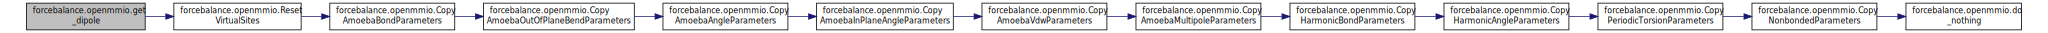
\includegraphics[width=350pt]{namespaceforcebalance_1_1openmmio_a8a2081dcaf027b9b9ab224e22680714d_cgraph}
\end{center}
\end{figure}


\hypertarget{namespaceforcebalance_1_1openmmio_a829487387c4b4a4817a2e3fc50242857}{\index{forcebalance\-::openmmio@{forcebalance\-::openmmio}!get\-\_\-multipoles@{get\-\_\-multipoles}}
\index{get\-\_\-multipoles@{get\-\_\-multipoles}!forcebalance::openmmio@{forcebalance\-::openmmio}}
\paragraph[{get\-\_\-multipoles}]{\setlength{\rightskip}{0pt plus 5cm}def forcebalance.\-openmmio.\-get\-\_\-multipoles (
\begin{DoxyParamCaption}
\item[{}]{simulation, }
\item[{}]{q = {\ttfamily None}, }
\item[{}]{mass = {\ttfamily None}, }
\item[{}]{positions = {\ttfamily None}, }
\item[{}]{rmcom = {\ttfamily True}}
\end{DoxyParamCaption}
)}}\label{namespaceforcebalance_1_1openmmio_a829487387c4b4a4817a2e3fc50242857}


Return the current multipole moments in Debye and Buckingham units. 



Definition at line 48 of file openmmio.\-py.

\hypertarget{namespaceforcebalance_1_1openmmio_a71e9c5b9d6a71839f5e04cd7ad7351db}{\index{forcebalance\-::openmmio@{forcebalance\-::openmmio}!Get\-Virtual\-Site\-Parameters@{Get\-Virtual\-Site\-Parameters}}
\index{Get\-Virtual\-Site\-Parameters@{Get\-Virtual\-Site\-Parameters}!forcebalance::openmmio@{forcebalance\-::openmmio}}
\paragraph[{Get\-Virtual\-Site\-Parameters}]{\setlength{\rightskip}{0pt plus 5cm}def forcebalance.\-openmmio.\-Get\-Virtual\-Site\-Parameters (
\begin{DoxyParamCaption}
\item[{}]{system}
\end{DoxyParamCaption}
)}}\label{namespaceforcebalance_1_1openmmio_a71e9c5b9d6a71839f5e04cd7ad7351db}


Return an array of all virtual site parameters in the system. 

Used for comparison purposes. 

Definition at line 194 of file openmmio.\-py.

\hypertarget{namespaceforcebalance_1_1openmmio_aa085594c11e9cd00ce71f5a8ead72b68}{\index{forcebalance\-::openmmio@{forcebalance\-::openmmio}!M\-T\-S\-V\-V\-V\-R\-Integrator@{M\-T\-S\-V\-V\-V\-R\-Integrator}}
\index{M\-T\-S\-V\-V\-V\-R\-Integrator@{M\-T\-S\-V\-V\-V\-R\-Integrator}!forcebalance::openmmio@{forcebalance\-::openmmio}}
\paragraph[{M\-T\-S\-V\-V\-V\-R\-Integrator}]{\setlength{\rightskip}{0pt plus 5cm}def forcebalance.\-openmmio.\-M\-T\-S\-V\-V\-V\-R\-Integrator (
\begin{DoxyParamCaption}
\item[{}]{temperature, }
\item[{}]{collision\-\_\-rate, }
\item[{}]{timestep, }
\item[{}]{system, }
\item[{}]{ninnersteps = {\ttfamily 4}}
\end{DoxyParamCaption}
)}}\label{namespaceforcebalance_1_1openmmio_aa085594c11e9cd00ce71f5a8ead72b68}


Create a multiple timestep velocity verlet with velocity randomization (V\-V\-V\-R) integrator. 

A\-R\-G\-U\-M\-E\-N\-T\-S

temperature (Quantity compatible with kelvin) -\/ the temperature collision\-\_\-rate (Quantity compatible with 1/picoseconds) -\/ the collision rate timestep (Quantity compatible with femtoseconds) -\/ the integration timestep system (simtk.\-openmm.\-System) -\/ system whose forces will be partitioned ninnersteps (int) -\/ number of inner timesteps (default\-: 4)

R\-E\-T\-U\-R\-N\-S

integrator (openmm.\-Custom\-Integrator) -\/ a V\-V\-V\-R integrator

N\-O\-T\-E\-S

This integrator is equivalent to a Langevin integrator in the velocity Verlet discretization with a timestep correction to ensure that the field-\/free diffusion constant is timestep invariant. The inner velocity Verlet discretization is transformed into a multiple timestep algorithm.

R\-E\-F\-E\-R\-E\-N\-C\-E\-S

V\-V\-V\-R Langevin integrator\-:
\begin{DoxyItemize}
\item \href{http://arxiv.org/abs/1301.3800}{\tt http\-://arxiv.\-org/abs/1301.\-3800}
\item \href{http://arxiv.org/abs/1107.2967}{\tt http\-://arxiv.\-org/abs/1107.\-2967} (to appear in P\-R\-X 2013)
\end{DoxyItemize}

T\-O\-D\-O

Move initialization of 'sigma' to setting the per-\/particle variables. 

Definition at line 357 of file openmmio.\-py.

\hypertarget{namespaceforcebalance_1_1openmmio_ac7c1f986acada081a7c24a5d77701a35}{\index{forcebalance\-::openmmio@{forcebalance\-::openmmio}!Prepare\-Virtual\-Sites@{Prepare\-Virtual\-Sites}}
\index{Prepare\-Virtual\-Sites@{Prepare\-Virtual\-Sites}!forcebalance::openmmio@{forcebalance\-::openmmio}}
\paragraph[{Prepare\-Virtual\-Sites}]{\setlength{\rightskip}{0pt plus 5cm}def forcebalance.\-openmmio.\-Prepare\-Virtual\-Sites (
\begin{DoxyParamCaption}
\item[{}]{system}
\end{DoxyParamCaption}
)}}\label{namespaceforcebalance_1_1openmmio_ac7c1f986acada081a7c24a5d77701a35}


Prepare a list of function wrappers and vsite parameters from the system. 



Definition at line 112 of file openmmio.\-py.

\hypertarget{namespaceforcebalance_1_1openmmio_af623fa5af97de6c6a0bc5f98ce8db432}{\index{forcebalance\-::openmmio@{forcebalance\-::openmmio}!Reset\-Virtual\-Sites@{Reset\-Virtual\-Sites}}
\index{Reset\-Virtual\-Sites@{Reset\-Virtual\-Sites}!forcebalance::openmmio@{forcebalance\-::openmmio}}
\paragraph[{Reset\-Virtual\-Sites}]{\setlength{\rightskip}{0pt plus 5cm}def forcebalance.\-openmmio.\-Reset\-Virtual\-Sites (
\begin{DoxyParamCaption}
\item[{}]{positions, }
\item[{}]{system}
\end{DoxyParamCaption}
)}}\label{namespaceforcebalance_1_1openmmio_af623fa5af97de6c6a0bc5f98ce8db432}


Given a set of Open\-M\-M-\/compatible positions and a System object, compute the correct virtual site positions according to the System. 



Definition at line 167 of file openmmio.\-py.

\hypertarget{namespaceforcebalance_1_1openmmio_a1f92d88085657ca5726f8925bfa68f6f}{\index{forcebalance\-::openmmio@{forcebalance\-::openmmio}!Reset\-Virtual\-Sites\-\_\-fast@{Reset\-Virtual\-Sites\-\_\-fast}}
\index{Reset\-Virtual\-Sites\-\_\-fast@{Reset\-Virtual\-Sites\-\_\-fast}!forcebalance::openmmio@{forcebalance\-::openmmio}}
\paragraph[{Reset\-Virtual\-Sites\-\_\-fast}]{\setlength{\rightskip}{0pt plus 5cm}def forcebalance.\-openmmio.\-Reset\-Virtual\-Sites\-\_\-fast (
\begin{DoxyParamCaption}
\item[{}]{positions, }
\item[{}]{vsinfo}
\end{DoxyParamCaption}
)}}\label{namespaceforcebalance_1_1openmmio_a1f92d88085657ca5726f8925bfa68f6f}


Given a set of Open\-M\-M-\/compatible positions and a System object, compute the correct virtual site positions according to the System. 



Definition at line 152 of file openmmio.\-py.

\hypertarget{namespaceforcebalance_1_1openmmio_a95d91538d72e354fc95433539c42450c}{\index{forcebalance\-::openmmio@{forcebalance\-::openmmio}!Set\-Amoeba\-Virtual\-Exclusions@{Set\-Amoeba\-Virtual\-Exclusions}}
\index{Set\-Amoeba\-Virtual\-Exclusions@{Set\-Amoeba\-Virtual\-Exclusions}!forcebalance::openmmio@{forcebalance\-::openmmio}}
\paragraph[{Set\-Amoeba\-Virtual\-Exclusions}]{\setlength{\rightskip}{0pt plus 5cm}def forcebalance.\-openmmio.\-Set\-Amoeba\-Virtual\-Exclusions (
\begin{DoxyParamCaption}
\item[{}]{system}
\end{DoxyParamCaption}
)}}\label{namespaceforcebalance_1_1openmmio_a95d91538d72e354fc95433539c42450c}


Definition at line 304 of file openmmio.\-py.

\hypertarget{namespaceforcebalance_1_1openmmio_a9f9fc56475dbfcc94a40fef6a84ed25f}{\index{forcebalance\-::openmmio@{forcebalance\-::openmmio}!Update\-Simulation\-Parameters@{Update\-Simulation\-Parameters}}
\index{Update\-Simulation\-Parameters@{Update\-Simulation\-Parameters}!forcebalance::openmmio@{forcebalance\-::openmmio}}
\paragraph[{Update\-Simulation\-Parameters}]{\setlength{\rightskip}{0pt plus 5cm}def forcebalance.\-openmmio.\-Update\-Simulation\-Parameters (
\begin{DoxyParamCaption}
\item[{}]{src\-\_\-system, }
\item[{}]{dest\-\_\-simulation}
\end{DoxyParamCaption}
)}}\label{namespaceforcebalance_1_1openmmio_a9f9fc56475dbfcc94a40fef6a84ed25f}


Definition at line 298 of file openmmio.\-py.



Here is the call graph for this function\-:
\nopagebreak
\begin{figure}[H]
\begin{center}
\leavevmode
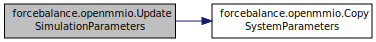
\includegraphics[width=350pt]{namespaceforcebalance_1_1openmmio_a9f9fc56475dbfcc94a40fef6a84ed25f_cgraph}
\end{center}
\end{figure}




\subsubsection{Variable Documentation}
\hypertarget{namespaceforcebalance_1_1openmmio_a1ec0ffb9266be80868bb69259349220d}{\index{forcebalance\-::openmmio@{forcebalance\-::openmmio}!logger@{logger}}
\index{logger@{logger}!forcebalance::openmmio@{forcebalance\-::openmmio}}
\paragraph[{logger}]{\setlength{\rightskip}{0pt plus 5cm}tuple forcebalance.\-openmmio.\-logger = get\-Logger(\-\_\-\-\_\-name\-\_\-\-\_\-)}}\label{namespaceforcebalance_1_1openmmio_a1ec0ffb9266be80868bb69259349220d}


Definition at line 29 of file openmmio.\-py.

\hypertarget{namespaceforcebalance_1_1openmmio_af225f2cfdcfd96ebd1d3175c8770a850}{\index{forcebalance\-::openmmio@{forcebalance\-::openmmio}!pdict@{pdict}}
\index{pdict@{pdict}!forcebalance::openmmio@{forcebalance\-::openmmio}}
\paragraph[{pdict}]{\setlength{\rightskip}{0pt plus 5cm}string forcebalance.\-openmmio.\-pdict = \char`\"{}X\-M\-L\-\_\-\-Override\char`\"{}}}\label{namespaceforcebalance_1_1openmmio_af225f2cfdcfd96ebd1d3175c8770a850}


pdict is a useless variable if the force field is X\-M\-L. 



Definition at line 436 of file openmmio.\-py.

\hypertarget{namespaceforcebalance_1_1openmmio_aeca37c08912f1a88339680ed75839530}{\index{forcebalance\-::openmmio@{forcebalance\-::openmmio}!suffix\-\_\-dict@{suffix\-\_\-dict}}
\index{suffix\-\_\-dict@{suffix\-\_\-dict}!forcebalance::openmmio@{forcebalance\-::openmmio}}
\paragraph[{suffix\-\_\-dict}]{\setlength{\rightskip}{0pt plus 5cm}dictionary forcebalance.\-openmmio.\-suffix\-\_\-dict}}\label{namespaceforcebalance_1_1openmmio_aeca37c08912f1a88339680ed75839530}
{\bfseries Initial value\-:}
\begin{DoxyCode}
1 = \{ \textcolor{stringliteral}{"HarmonicBondForce"} : \{\textcolor{stringliteral}{"Bond"} : [\textcolor{stringliteral}{"class1"},\textcolor{stringliteral}{"class2"}]\},
2                 \textcolor{stringliteral}{"HarmonicAngleForce"} : \{\textcolor{stringliteral}{"Angle"} : [\textcolor{stringliteral}{"class1"},\textcolor{stringliteral}{"class2"},\textcolor{stringliteral}{"class3"}],\},
3                 \textcolor{stringliteral}{"PeriodicTorsionForce"} : \{\textcolor{stringliteral}{"Proper"} : [\textcolor{stringliteral}{"class1"},\textcolor{stringliteral}{"class2"},\textcolor{stringliteral}{"class3"},\textcolor{stringliteral}{"class4"}],\},
4                 \textcolor{stringliteral}{"NonbondedForce"} : \{\textcolor{stringliteral}{"Atom"}: [\textcolor{stringliteral}{"type"}]\},
5                 \textcolor{stringliteral}{"AmoebaBondForce"} : \{\textcolor{stringliteral}{"Bond"} : [\textcolor{stringliteral}{"class1"},\textcolor{stringliteral}{"class2"}]\},
6                 \textcolor{stringliteral}{"AmoebaAngleForce"} : \{\textcolor{stringliteral}{"Angle"} : [\textcolor{stringliteral}{"class1"},\textcolor{stringliteral}{"class2"},\textcolor{stringliteral}{"class3"}]\},
7                 \textcolor{stringliteral}{"AmoebaStretchBendForce"} : \{\textcolor{stringliteral}{"StretchBend"} : [\textcolor{stringliteral}{"class1"},\textcolor{stringliteral}{"class2"},\textcolor{stringliteral}{"class3"}]\},
8                 \textcolor{stringliteral}{"AmoebaVdwForce"} : \{\textcolor{stringliteral}{"Vdw"} : [\textcolor{stringliteral}{"class"}]\},
9                 \textcolor{stringliteral}{"AmoebaMultipoleForce"} : \{\textcolor{stringliteral}{"Multipole"} : [\textcolor{stringliteral}{"type"},\textcolor{stringliteral}{"kz"},\textcolor{stringliteral}{"kx"}], \textcolor{stringliteral}{"Polarize"} : [\textcolor{stringliteral}{"type"}]\},
10                 \textcolor{stringliteral}{"AmoebaUreyBradleyForce"} : \{\textcolor{stringliteral}{"UreyBradley"} : [\textcolor{stringliteral}{"class1"},\textcolor{stringliteral}{"class2"},\textcolor{stringliteral}{"class3"}]\},
11                 \textcolor{stringliteral}{"Residues.Residue"} : \{\textcolor{stringliteral}{"VirtualSite"} : [\textcolor{stringliteral}{"index"}]\}
12                 \}
\end{DoxyCode}


Definition at line 422 of file openmmio.\-py.


\hypertarget{namespaceforcebalance_1_1optimizer}{\subsection{forcebalance.\-optimizer Namespace Reference}
\label{namespaceforcebalance_1_1optimizer}\index{forcebalance.\-optimizer@{forcebalance.\-optimizer}}
}


Optimization algorithms.  


\subsubsection*{Classes}
\begin{DoxyCompactItemize}
\item 
class \hyperlink{classforcebalance_1_1optimizer_1_1Optimizer}{Optimizer}
\begin{DoxyCompactList}\small\item\em \hyperlink{classforcebalance_1_1optimizer_1_1Optimizer}{Optimizer} class. \end{DoxyCompactList}\end{DoxyCompactItemize}
\subsubsection*{Functions}
\begin{DoxyCompactItemize}
\item 
def \hyperlink{namespaceforcebalance_1_1optimizer_ae1f6c649703a22b2f767a5f6bf53297b}{Counter}
\item 
def \hyperlink{namespaceforcebalance_1_1optimizer_a1b6394e430a899f19957694a173e9150}{First}
\item 
def \hyperlink{namespaceforcebalance_1_1optimizer_ab43948ecf30c90d319e0c0b107fe484a}{Good\-Step}
\end{DoxyCompactItemize}
\subsubsection*{Variables}
\begin{DoxyCompactItemize}
\item 
tuple \hyperlink{namespaceforcebalance_1_1optimizer_a8c7d22696df2debf02ce9e3bb35349fd}{logger} = get\-Logger(\-\_\-\-\_\-name\-\_\-\-\_\-)
\item 
int \hyperlink{namespaceforcebalance_1_1optimizer_aaf93ec60981b2c73b2f36a4cf5c5874f}{I\-T\-E\-R\-A\-T\-I\-O\-N} = 0
\item 
int \hyperlink{namespaceforcebalance_1_1optimizer_a7b0cf561a0ec911ee4b217cb0b05a28e}{G\-O\-O\-D\-S\-T\-E\-P} = 0
\item 
int \hyperlink{namespaceforcebalance_1_1optimizer_a42aec8ce55b20c7ffdd69bf188ebbf44}{I\-T\-E\-R\-I\-N\-I\-T} = 0
\end{DoxyCompactItemize}


\subsubsection{Detailed Description}
Optimization algorithms. My current implementation is to have a single optimizer class with several methods contained inside.

\begin{DoxyAuthor}{Author}
Lee-\/\-Ping Wang 
\end{DoxyAuthor}
\begin{DoxyDate}{Date}
12/2011 
\end{DoxyDate}


\subsubsection{Function Documentation}
\hypertarget{namespaceforcebalance_1_1optimizer_ae1f6c649703a22b2f767a5f6bf53297b}{\index{forcebalance\-::optimizer@{forcebalance\-::optimizer}!Counter@{Counter}}
\index{Counter@{Counter}!forcebalance::optimizer@{forcebalance\-::optimizer}}
\paragraph[{Counter}]{\setlength{\rightskip}{0pt plus 5cm}def forcebalance.\-optimizer.\-Counter (
\begin{DoxyParamCaption}
{}
\end{DoxyParamCaption}
)}}\label{namespaceforcebalance_1_1optimizer_ae1f6c649703a22b2f767a5f6bf53297b}


Definition at line 32 of file optimizer.\-py.

\hypertarget{namespaceforcebalance_1_1optimizer_a1b6394e430a899f19957694a173e9150}{\index{forcebalance\-::optimizer@{forcebalance\-::optimizer}!First@{First}}
\index{First@{First}!forcebalance::optimizer@{forcebalance\-::optimizer}}
\paragraph[{First}]{\setlength{\rightskip}{0pt plus 5cm}def forcebalance.\-optimizer.\-First (
\begin{DoxyParamCaption}
{}
\end{DoxyParamCaption}
)}}\label{namespaceforcebalance_1_1optimizer_a1b6394e430a899f19957694a173e9150}


Definition at line 36 of file optimizer.\-py.

\hypertarget{namespaceforcebalance_1_1optimizer_ab43948ecf30c90d319e0c0b107fe484a}{\index{forcebalance\-::optimizer@{forcebalance\-::optimizer}!Good\-Step@{Good\-Step}}
\index{Good\-Step@{Good\-Step}!forcebalance::optimizer@{forcebalance\-::optimizer}}
\paragraph[{Good\-Step}]{\setlength{\rightskip}{0pt plus 5cm}def forcebalance.\-optimizer.\-Good\-Step (
\begin{DoxyParamCaption}
{}
\end{DoxyParamCaption}
)}}\label{namespaceforcebalance_1_1optimizer_ab43948ecf30c90d319e0c0b107fe484a}


Definition at line 40 of file optimizer.\-py.



\subsubsection{Variable Documentation}
\hypertarget{namespaceforcebalance_1_1optimizer_a7b0cf561a0ec911ee4b217cb0b05a28e}{\index{forcebalance\-::optimizer@{forcebalance\-::optimizer}!G\-O\-O\-D\-S\-T\-E\-P@{G\-O\-O\-D\-S\-T\-E\-P}}
\index{G\-O\-O\-D\-S\-T\-E\-P@{G\-O\-O\-D\-S\-T\-E\-P}!forcebalance::optimizer@{forcebalance\-::optimizer}}
\paragraph[{G\-O\-O\-D\-S\-T\-E\-P}]{\setlength{\rightskip}{0pt plus 5cm}int forcebalance.\-optimizer.\-G\-O\-O\-D\-S\-T\-E\-P = 0}}\label{namespaceforcebalance_1_1optimizer_a7b0cf561a0ec911ee4b217cb0b05a28e}


Definition at line 27 of file optimizer.\-py.

\hypertarget{namespaceforcebalance_1_1optimizer_aaf93ec60981b2c73b2f36a4cf5c5874f}{\index{forcebalance\-::optimizer@{forcebalance\-::optimizer}!I\-T\-E\-R\-A\-T\-I\-O\-N@{I\-T\-E\-R\-A\-T\-I\-O\-N}}
\index{I\-T\-E\-R\-A\-T\-I\-O\-N@{I\-T\-E\-R\-A\-T\-I\-O\-N}!forcebalance::optimizer@{forcebalance\-::optimizer}}
\paragraph[{I\-T\-E\-R\-A\-T\-I\-O\-N}]{\setlength{\rightskip}{0pt plus 5cm}int forcebalance.\-optimizer.\-I\-T\-E\-R\-A\-T\-I\-O\-N = 0}}\label{namespaceforcebalance_1_1optimizer_aaf93ec60981b2c73b2f36a4cf5c5874f}


Definition at line 25 of file optimizer.\-py.

\hypertarget{namespaceforcebalance_1_1optimizer_a42aec8ce55b20c7ffdd69bf188ebbf44}{\index{forcebalance\-::optimizer@{forcebalance\-::optimizer}!I\-T\-E\-R\-I\-N\-I\-T@{I\-T\-E\-R\-I\-N\-I\-T}}
\index{I\-T\-E\-R\-I\-N\-I\-T@{I\-T\-E\-R\-I\-N\-I\-T}!forcebalance::optimizer@{forcebalance\-::optimizer}}
\paragraph[{I\-T\-E\-R\-I\-N\-I\-T}]{\setlength{\rightskip}{0pt plus 5cm}int forcebalance.\-optimizer.\-I\-T\-E\-R\-I\-N\-I\-T = 0}}\label{namespaceforcebalance_1_1optimizer_a42aec8ce55b20c7ffdd69bf188ebbf44}


Definition at line 30 of file optimizer.\-py.

\hypertarget{namespaceforcebalance_1_1optimizer_a8c7d22696df2debf02ce9e3bb35349fd}{\index{forcebalance\-::optimizer@{forcebalance\-::optimizer}!logger@{logger}}
\index{logger@{logger}!forcebalance::optimizer@{forcebalance\-::optimizer}}
\paragraph[{logger}]{\setlength{\rightskip}{0pt plus 5cm}tuple forcebalance.\-optimizer.\-logger = get\-Logger(\-\_\-\-\_\-name\-\_\-\-\_\-)}}\label{namespaceforcebalance_1_1optimizer_a8c7d22696df2debf02ce9e3bb35349fd}


Definition at line 22 of file optimizer.\-py.


\hypertarget{namespaceforcebalance_1_1output}{\subsection{forcebalance.\-output Namespace Reference}
\label{namespaceforcebalance_1_1output}\index{forcebalance.\-output@{forcebalance.\-output}}
}
\subsubsection*{Classes}
\begin{DoxyCompactItemize}
\item 
class \hyperlink{classforcebalance_1_1output_1_1RawStreamHandler}{Raw\-Stream\-Handler}
\begin{DoxyCompactList}\small\item\em Exactly like output.\-Stream\-Handler except it does no extra formatting before sending logging messages to the stream. \end{DoxyCompactList}\item 
class \hyperlink{classforcebalance_1_1output_1_1RawFileHandler}{Raw\-File\-Handler}
\begin{DoxyCompactList}\small\item\em Exactly like output.\-File\-Handler except it does no extra formatting before sending logging messages to the file. \end{DoxyCompactList}\item 
class \hyperlink{classforcebalance_1_1output_1_1CleanFileHandler}{Clean\-File\-Handler}
\begin{DoxyCompactList}\small\item\em File handler that does not write terminal escape codes to files. \end{DoxyCompactList}\end{DoxyCompactItemize}
\subsubsection*{Variables}
\begin{DoxyCompactItemize}
\item 
tuple \hyperlink{namespaceforcebalance_1_1output_a870a4f031710283f04ba9eb0908fa5fa}{logger} = get\-Logger('forcebalance')
\end{DoxyCompactItemize}


\subsubsection{Variable Documentation}
\hypertarget{namespaceforcebalance_1_1output_a870a4f031710283f04ba9eb0908fa5fa}{\index{forcebalance\-::output@{forcebalance\-::output}!logger@{logger}}
\index{logger@{logger}!forcebalance::output@{forcebalance\-::output}}
\paragraph[{logger}]{\setlength{\rightskip}{0pt plus 5cm}tuple forcebalance.\-output.\-logger = get\-Logger('forcebalance')}}\label{namespaceforcebalance_1_1output_a870a4f031710283f04ba9eb0908fa5fa}


Definition at line 5 of file output.\-py.


\hypertarget{namespaceforcebalance_1_1parser}{\subsection{forcebalance\-:\-:parser \-Namespace \-Reference}
\label{namespaceforcebalance_1_1parser}\index{forcebalance\-::parser@{forcebalance\-::parser}}
}


\-Input file parser for \-Force\-Balance jobs.  


\subsubsection*{\-Functions}
\begin{DoxyCompactItemize}
\item 
def \hyperlink{namespaceforcebalance_1_1parser_aef8b51dba6bb9767a9a956319eb3cc08}{read\-\_\-mvals}
\item 
def \hyperlink{namespaceforcebalance_1_1parser_a56fb1e139dad24bac29f25a3870765ca}{read\-\_\-pvals}
\item 
def \hyperlink{namespaceforcebalance_1_1parser_a94c3f1acd06b640db3042dc45e32af8e}{read\-\_\-priors}
\item 
def \hyperlink{namespaceforcebalance_1_1parser_a10827b0b21d0463bc9e786f161a02654}{read\-\_\-internals}
\item 
def \hyperlink{namespaceforcebalance_1_1parser_a00a8cb7b534312c13b11d4bb39bb3959}{printsection}
\begin{DoxyCompactList}\small\item\em \-Print out a section of the input file in a parser-\/compliant and readable format. \end{DoxyCompactList}\item 
def \hyperlink{namespaceforcebalance_1_1parser_ac184c809737a27f35530020322431f7c}{parse\-\_\-inputs}
\begin{DoxyCompactList}\small\item\em \-Parse through the input file and read all user-\/supplied options. \end{DoxyCompactList}\end{DoxyCompactItemize}
\subsubsection*{\-Variables}
\begin{DoxyCompactItemize}
\item 
tuple \hyperlink{namespaceforcebalance_1_1parser_a0e0761161c5ff444c7afbcc9157cd710}{logger} = get\-Logger(\-\_\-\-\_\-name\-\_\-\-\_\-)
\item 
dictionary \hyperlink{namespaceforcebalance_1_1parser_a2ac3b892432d1c614c32eebeb8de41c5}{gen\-\_\-opts\-\_\-types}
\begin{DoxyCompactList}\small\item\em \-Default general options. \end{DoxyCompactList}\item 
dictionary \hyperlink{namespaceforcebalance_1_1parser_a1725a6ea3c588046339f9476f3e3f32e}{tgt\-\_\-opts\-\_\-types}
\begin{DoxyCompactList}\small\item\em \-Default fitting target options. \end{DoxyCompactList}\item 
tuple \hyperlink{namespaceforcebalance_1_1parser_ab0f8ac22b808f515531c830439d70bbb}{all\-\_\-opts\-\_\-names} = list(itertools.\-chain($\ast$\mbox{[}i.\-keys() for i in gen\-\_\-opts\-\_\-types.\-values()\mbox{]}))
\item 
list \hyperlink{namespaceforcebalance_1_1parser_af730ef69e27de8ffbf475f844c5c2d5f}{iocc} = \mbox{[}$\,$\mbox{]}
\begin{DoxyCompactList}\small\item\em \-Check for uniqueness of option names. \end{DoxyCompactList}\item 
dictionary \hyperlink{namespaceforcebalance_1_1parser_a807ea3a28fedbdfd494f5cc8da063202}{gen\-\_\-opts\-\_\-defaults} = \{\}
\begin{DoxyCompactList}\small\item\em \-Default general options -\/ basically a collapsed veresion of gen\-\_\-opts\-\_\-types. \end{DoxyCompactList}\item 
dictionary \hyperlink{namespaceforcebalance_1_1parser_abb7a7e9723de629aa97727a85bcdbad1}{subdict} = \{\}
\item 
dictionary \hyperlink{namespaceforcebalance_1_1parser_ad2c80e2b742fbd9594fd813dd51550e6}{tgt\-\_\-opts\-\_\-defaults} = \{\}
\begin{DoxyCompactList}\small\item\em \-Default target options -\/ basically a collapsed version of tgt\-\_\-opts\-\_\-types. \end{DoxyCompactList}\item 
dictionary \hyperlink{namespaceforcebalance_1_1parser_a37193d7ceabbf07a61e65677372b7dab}{bkwd} = \{\char`\"{}simtype\char`\"{} \-: \char`\"{}type\char`\"{}, \char`\"{}masterfile\char`\"{} \-: \char`\"{}binding\-\_\-txt\char`\"{}\}
\begin{DoxyCompactList}\small\item\em \-Option maps for maintaining backward compatibility. \end{DoxyCompactList}\item 
list \hyperlink{namespaceforcebalance_1_1parser_a525ac339b645dbfb9fbb7cc672712504}{mainsections} = \mbox{[}\char`\"{}\-S\-I\-M\-U\-L\-A\-T\-I\-O\-N\char`\"{},\char`\"{}\-T\-A\-R\-G\-E\-T\char`\"{},\char`\"{}\-O\-P\-T\-I\-O\-N\-S\char`\"{},\char`\"{}\-E\-N\-D\char`\"{},\char`\"{}\-N\-O\-N\-E\char`\"{}\mbox{]}
\begin{DoxyCompactList}\small\item\em \-Listing of sections in the input file. \end{DoxyCompactList}\item 
dictionary \hyperlink{namespaceforcebalance_1_1parser_af0a8dc5cdc54cc88ded3ee3b46d71672}{\-Pars\-Tab}
\begin{DoxyCompactList}\small\item\em \-Pars\-Tab that refers to subsection parsers. \end{DoxyCompactList}\end{DoxyCompactItemize}


\subsubsection{\-Detailed \-Description}
\-Input file parser for \-Force\-Balance jobs. \-Additionally, the location for all default options.

\-Although \-I will do my best to write good documentation, for many programs the input parser becomes the most up-\/to-\/date source for documentation. \-So this is a great place to write lots of comments for those who implement new functionality.

\-There are two types of sections for options -\/ \-G\-E\-N\-E\-R\-A\-L and \-T\-A\-R\-G\-E\-T. \-Since there can be many fitting targets within a single job (i.\-e. we may wish to fit water trimers and hexamers, which constitutes two fitting targets) the input is organized into sections, like so\-:

\$options\par
 gen\-\_\-option\-\_\-1 \-Big\par
 gen\-\_\-option\-\_\-2 \-Mao\par
 \$target\par
 tgt\-\_\-option\-\_\-1 \-Sniffy\par
 tgt\-\_\-option\-\_\-2 \-Schmao\par
 \$target\par
 tgt\-\_\-option\-\_\-1 \-Nifty\par
 tgt\-\_\-option\-\_\-2 \-Jiffy\par
 \$end

\-In this case, two sets of target options are generated in addition to the general option.

(\-Note\-: \char`\"{}\-Target\char`\"{} used to be called \char`\"{}\-Simulation\char`\"{}. \-Backwards compatibility is maintained.)

\-Each option is meant to be parsed as a certain variable type.


\begin{DoxyItemize}
\item \-String option values are read in directly; note that only the first two words in the line are processed
\item \-Some strings are capitalized when they are read in; this is mainly for function tables like \-Opt\-Tab and \-Tgt\-Tab
\item \-List option types will pick up all of the words on the line and use them as values, plus if the option occurs more than once it will aggregate all of the values.
\item \-Integer and float option types are read in a pretty straightforward way
\item \-Boolean option types are always set to true, unless the second word is '0', 'no', or 'false' (not case sensitive)
\item \-Section option types are meant to treat more elaborate inputs, such as the user pasting in output parameters from a previous job as input, or a specification of internal coordinate system. \-I imagine that for every section type \-I would have to write my own parser. \-Maybe a \-Pars\-Tab of parsing functions would work. \-:)
\end{DoxyItemize}

\-To add a new option, simply add it to the dictionaries below and give it a default value if desired. \-If you add an entirely new type, make sure to implement the interpretation of that type in the parse\-\_\-inputs function.

\begin{DoxyAuthor}{\-Author}
\-Lee-\/\-Ping \-Wang 
\end{DoxyAuthor}
\begin{DoxyDate}{\-Date}
11/2012 
\end{DoxyDate}


\subsubsection{\-Function \-Documentation}
\hypertarget{namespaceforcebalance_1_1parser_ac184c809737a27f35530020322431f7c}{\index{forcebalance\-::parser@{forcebalance\-::parser}!parse\-\_\-inputs@{parse\-\_\-inputs}}
\index{parse\-\_\-inputs@{parse\-\_\-inputs}!forcebalance::parser@{forcebalance\-::parser}}
\paragraph[{parse\-\_\-inputs}]{\setlength{\rightskip}{0pt plus 5cm}def {\bf forcebalance.\-parser.\-parse\-\_\-inputs} (
\begin{DoxyParamCaption}
\item[{}]{input\-\_\-file = {\ttfamily \-None}}
\end{DoxyParamCaption}
)}}\label{namespaceforcebalance_1_1parser_ac184c809737a27f35530020322431f7c}


\-Parse through the input file and read all user-\/supplied options. 

\-This is usually the first thing that happens when an executable script is called. \-Our parser first loads the default options, and then updates these options as it encounters keywords.

\-Each keyword corresponds to a variable type; each variable type (e.\-g. string, integer, float, boolean) is treated differently. \-For more elaborate inputs, there is a 'section' variable type.

\-There is only one set of general options, but multiple sets of target options. \-Each target has its own section delimited by the {\itshape \$target\/} keyword, and we build a list of target options.


\begin{DoxyParams}[1]{\-Parameters}
\mbox{\tt in}  & {\em input\-\_\-file} & \-The name of the input file. \\
\hline
\end{DoxyParams}
\begin{DoxyReturn}{\-Returns}
options \-General options. 

tgt\-\_\-opts \-List of fitting target options.
\end{DoxyReturn}
\begin{DoxyRefDesc}{\-Todo}
\item[\hyperlink{todo__todo000017}{\-Todo}]\-Implement internal coordinates. 

\-Implement sampling correction. 

\-Implement charge groups. \end{DoxyRefDesc}


\-Definition at line 396 of file parser.\-py.



\-Here is the call graph for this function\-:\nopagebreak
\begin{figure}[H]
\begin{center}
\leavevmode
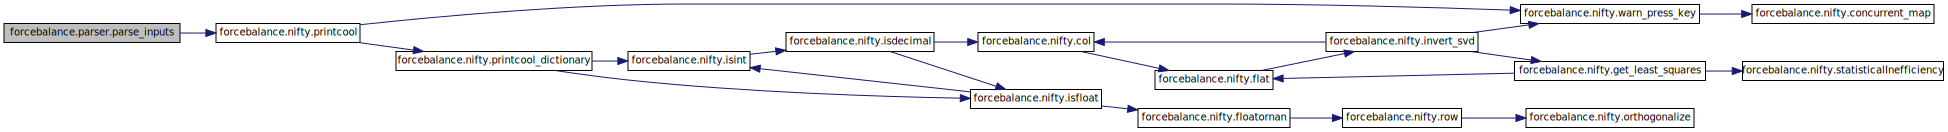
\includegraphics[width=350pt]{namespaceforcebalance_1_1parser_ac184c809737a27f35530020322431f7c_cgraph}
\end{center}
\end{figure}


\hypertarget{namespaceforcebalance_1_1parser_a00a8cb7b534312c13b11d4bb39bb3959}{\index{forcebalance\-::parser@{forcebalance\-::parser}!printsection@{printsection}}
\index{printsection@{printsection}!forcebalance::parser@{forcebalance\-::parser}}
\paragraph[{printsection}]{\setlength{\rightskip}{0pt plus 5cm}def {\bf forcebalance.\-parser.\-printsection} (
\begin{DoxyParamCaption}
\item[{}]{heading, }
\item[{}]{optdict, }
\item[{}]{typedict}
\end{DoxyParamCaption}
)}}\label{namespaceforcebalance_1_1parser_a00a8cb7b534312c13b11d4bb39bb3959}


\-Print out a section of the input file in a parser-\/compliant and readable format. 

\-At the time of writing of this function, it's mainly intended to be called by \-Make\-Input\-File.\-py. \-The heading is printed first (it is something like \$options or \$target). \-Then it loops through the variable types (strings, allcaps, etc...) and the keys in each variable type. \-The one-\/line description of each key is printed out as a comment, and then the key itself is printed out along with the value provided in optdict. \-If optdict is \-None, then the default value is printed out instead.


\begin{DoxyParams}[1]{\-Parameters}
\mbox{\tt in}  & {\em heading} & \-Heading, either \$options or \$target \\
\hline
\mbox{\tt in}  & {\em optdict} & \-Options dictionary or \-None. \\
\hline
\mbox{\tt in}  & {\em typedict} & \-Option type dictionary, either gen\-\_\-opts\-\_\-types or tgt\-\_\-opts\-\_\-types specified in this file. \\
\hline
\end{DoxyParams}
\begin{DoxyReturn}{\-Returns}
\-Answer \-List of strings for the section that we are printing out. 
\end{DoxyReturn}


\-Definition at line 299 of file parser.\-py.



\-Here is the call graph for this function\-:\nopagebreak
\begin{figure}[H]
\begin{center}
\leavevmode
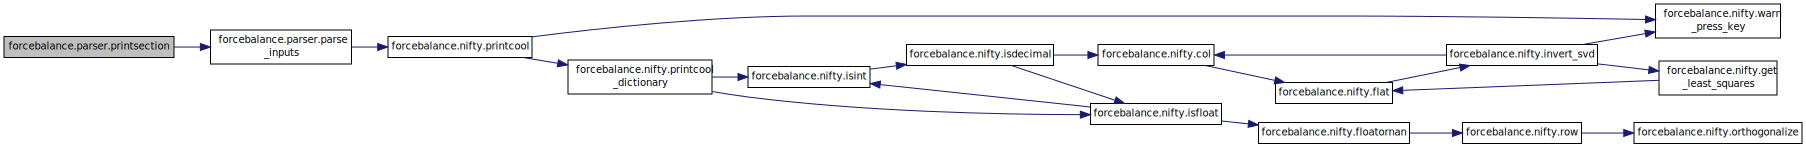
\includegraphics[width=350pt]{namespaceforcebalance_1_1parser_a00a8cb7b534312c13b11d4bb39bb3959_cgraph}
\end{center}
\end{figure}


\hypertarget{namespaceforcebalance_1_1parser_a10827b0b21d0463bc9e786f161a02654}{\index{forcebalance\-::parser@{forcebalance\-::parser}!read\-\_\-internals@{read\-\_\-internals}}
\index{read\-\_\-internals@{read\-\_\-internals}!forcebalance::parser@{forcebalance\-::parser}}
\paragraph[{read\-\_\-internals}]{\setlength{\rightskip}{0pt plus 5cm}def {\bf forcebalance.\-parser.\-read\-\_\-internals} (
\begin{DoxyParamCaption}
\item[{}]{fobj}
\end{DoxyParamCaption}
)}}\label{namespaceforcebalance_1_1parser_a10827b0b21d0463bc9e786f161a02654}


\-Definition at line 273 of file parser.\-py.

\hypertarget{namespaceforcebalance_1_1parser_aef8b51dba6bb9767a9a956319eb3cc08}{\index{forcebalance\-::parser@{forcebalance\-::parser}!read\-\_\-mvals@{read\-\_\-mvals}}
\index{read\-\_\-mvals@{read\-\_\-mvals}!forcebalance::parser@{forcebalance\-::parser}}
\paragraph[{read\-\_\-mvals}]{\setlength{\rightskip}{0pt plus 5cm}def {\bf forcebalance.\-parser.\-read\-\_\-mvals} (
\begin{DoxyParamCaption}
\item[{}]{fobj}
\end{DoxyParamCaption}
)}}\label{namespaceforcebalance_1_1parser_aef8b51dba6bb9767a9a956319eb3cc08}


\-Definition at line 248 of file parser.\-py.



\-Here is the call graph for this function\-:\nopagebreak
\begin{figure}[H]
\begin{center}
\leavevmode
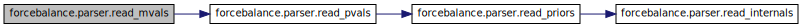
\includegraphics[width=350pt]{namespaceforcebalance_1_1parser_aef8b51dba6bb9767a9a956319eb3cc08_cgraph}
\end{center}
\end{figure}


\hypertarget{namespaceforcebalance_1_1parser_a94c3f1acd06b640db3042dc45e32af8e}{\index{forcebalance\-::parser@{forcebalance\-::parser}!read\-\_\-priors@{read\-\_\-priors}}
\index{read\-\_\-priors@{read\-\_\-priors}!forcebalance::parser@{forcebalance\-::parser}}
\paragraph[{read\-\_\-priors}]{\setlength{\rightskip}{0pt plus 5cm}def {\bf forcebalance.\-parser.\-read\-\_\-priors} (
\begin{DoxyParamCaption}
\item[{}]{fobj}
\end{DoxyParamCaption}
)}}\label{namespaceforcebalance_1_1parser_a94c3f1acd06b640db3042dc45e32af8e}


\-Definition at line 264 of file parser.\-py.



\-Here is the call graph for this function\-:\nopagebreak
\begin{figure}[H]
\begin{center}
\leavevmode
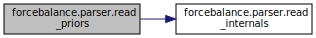
\includegraphics[width=350pt]{namespaceforcebalance_1_1parser_a94c3f1acd06b640db3042dc45e32af8e_cgraph}
\end{center}
\end{figure}


\hypertarget{namespaceforcebalance_1_1parser_a56fb1e139dad24bac29f25a3870765ca}{\index{forcebalance\-::parser@{forcebalance\-::parser}!read\-\_\-pvals@{read\-\_\-pvals}}
\index{read\-\_\-pvals@{read\-\_\-pvals}!forcebalance::parser@{forcebalance\-::parser}}
\paragraph[{read\-\_\-pvals}]{\setlength{\rightskip}{0pt plus 5cm}def {\bf forcebalance.\-parser.\-read\-\_\-pvals} (
\begin{DoxyParamCaption}
\item[{}]{fobj}
\end{DoxyParamCaption}
)}}\label{namespaceforcebalance_1_1parser_a56fb1e139dad24bac29f25a3870765ca}


\-Definition at line 256 of file parser.\-py.



\-Here is the call graph for this function\-:\nopagebreak
\begin{figure}[H]
\begin{center}
\leavevmode
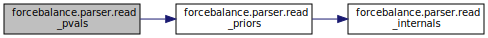
\includegraphics[width=350pt]{namespaceforcebalance_1_1parser_a56fb1e139dad24bac29f25a3870765ca_cgraph}
\end{center}
\end{figure}




\subsubsection{\-Variable \-Documentation}
\hypertarget{namespaceforcebalance_1_1parser_ab0f8ac22b808f515531c830439d70bbb}{\index{forcebalance\-::parser@{forcebalance\-::parser}!all\-\_\-opts\-\_\-names@{all\-\_\-opts\-\_\-names}}
\index{all\-\_\-opts\-\_\-names@{all\-\_\-opts\-\_\-names}!forcebalance::parser@{forcebalance\-::parser}}
\paragraph[{all\-\_\-opts\-\_\-names}]{\setlength{\rightskip}{0pt plus 5cm}tuple {\bf forcebalance\-::parser\-::all\-\_\-opts\-\_\-names} = list(itertools.\-chain($\ast$\mbox{[}i.\-keys() for i in gen\-\_\-opts\-\_\-types.\-values()\mbox{]}))}}\label{namespaceforcebalance_1_1parser_ab0f8ac22b808f515531c830439d70bbb}


\-Definition at line 213 of file parser.\-py.

\hypertarget{namespaceforcebalance_1_1parser_a37193d7ceabbf07a61e65677372b7dab}{\index{forcebalance\-::parser@{forcebalance\-::parser}!bkwd@{bkwd}}
\index{bkwd@{bkwd}!forcebalance::parser@{forcebalance\-::parser}}
\paragraph[{bkwd}]{\setlength{\rightskip}{0pt plus 5cm}dictionary {\bf forcebalance\-::parser\-::bkwd} = \{\char`\"{}simtype\char`\"{} \-: \char`\"{}type\char`\"{}, \char`\"{}masterfile\char`\"{} \-: \char`\"{}binding\-\_\-txt\char`\"{}\}}}\label{namespaceforcebalance_1_1parser_a37193d7ceabbf07a61e65677372b7dab}


\-Option maps for maintaining backward compatibility. 



\-Definition at line 243 of file parser.\-py.

\hypertarget{namespaceforcebalance_1_1parser_a807ea3a28fedbdfd494f5cc8da063202}{\index{forcebalance\-::parser@{forcebalance\-::parser}!gen\-\_\-opts\-\_\-defaults@{gen\-\_\-opts\-\_\-defaults}}
\index{gen\-\_\-opts\-\_\-defaults@{gen\-\_\-opts\-\_\-defaults}!forcebalance::parser@{forcebalance\-::parser}}
\paragraph[{gen\-\_\-opts\-\_\-defaults}]{\setlength{\rightskip}{0pt plus 5cm}dictionary {\bf forcebalance\-::parser\-::gen\-\_\-opts\-\_\-defaults} = \{\}}}\label{namespaceforcebalance_1_1parser_a807ea3a28fedbdfd494f5cc8da063202}


\-Default general options -\/ basically a collapsed veresion of gen\-\_\-opts\-\_\-types. 



\-Definition at line 227 of file parser.\-py.

\hypertarget{namespaceforcebalance_1_1parser_a2ac3b892432d1c614c32eebeb8de41c5}{\index{forcebalance\-::parser@{forcebalance\-::parser}!gen\-\_\-opts\-\_\-types@{gen\-\_\-opts\-\_\-types}}
\index{gen\-\_\-opts\-\_\-types@{gen\-\_\-opts\-\_\-types}!forcebalance::parser@{forcebalance\-::parser}}
\paragraph[{gen\-\_\-opts\-\_\-types}]{\setlength{\rightskip}{0pt plus 5cm}dictionary {\bf forcebalance\-::parser\-::gen\-\_\-opts\-\_\-types}}}\label{namespaceforcebalance_1_1parser_a2ac3b892432d1c614c32eebeb8de41c5}


\-Default general options. 

\-Note that the documentation is included in part of the key; this will aid in automatic doc-\/extraction. \-:) \-In the 5-\/tuple we have\-: \-Default value, priority (larger number means printed first), short docstring, description of scope, list of filter strings for pulling out pertinent targets (\-Make\-Input\-File.\-py) 

\-Definition at line 65 of file parser.\-py.

\hypertarget{namespaceforcebalance_1_1parser_af730ef69e27de8ffbf475f844c5c2d5f}{\index{forcebalance\-::parser@{forcebalance\-::parser}!iocc@{iocc}}
\index{iocc@{iocc}!forcebalance::parser@{forcebalance\-::parser}}
\paragraph[{iocc}]{\setlength{\rightskip}{0pt plus 5cm}list {\bf forcebalance\-::parser\-::iocc} = \mbox{[}$\,$\mbox{]}}}\label{namespaceforcebalance_1_1parser_af730ef69e27de8ffbf475f844c5c2d5f}


\-Check for uniqueness of option names. 



\-Definition at line 216 of file parser.\-py.

\hypertarget{namespaceforcebalance_1_1parser_a0e0761161c5ff444c7afbcc9157cd710}{\index{forcebalance\-::parser@{forcebalance\-::parser}!logger@{logger}}
\index{logger@{logger}!forcebalance::parser@{forcebalance\-::parser}}
\paragraph[{logger}]{\setlength{\rightskip}{0pt plus 5cm}tuple {\bf forcebalance\-::parser\-::logger} = get\-Logger(\-\_\-\-\_\-name\-\_\-\-\_\-)}}\label{namespaceforcebalance_1_1parser_a0e0761161c5ff444c7afbcc9157cd710}


\-Definition at line 60 of file parser.\-py.

\hypertarget{namespaceforcebalance_1_1parser_a525ac339b645dbfb9fbb7cc672712504}{\index{forcebalance\-::parser@{forcebalance\-::parser}!mainsections@{mainsections}}
\index{mainsections@{mainsections}!forcebalance::parser@{forcebalance\-::parser}}
\paragraph[{mainsections}]{\setlength{\rightskip}{0pt plus 5cm}list {\bf forcebalance\-::parser\-::mainsections} = \mbox{[}\char`\"{}\-S\-I\-M\-U\-L\-A\-T\-I\-O\-N\char`\"{},\char`\"{}\-T\-A\-R\-G\-E\-T\char`\"{},\char`\"{}\-O\-P\-T\-I\-O\-N\-S\char`\"{},\char`\"{}\-E\-N\-D\char`\"{},\char`\"{}\-N\-O\-N\-E\char`\"{}\mbox{]}}}\label{namespaceforcebalance_1_1parser_a525ac339b645dbfb9fbb7cc672712504}


\-Listing of sections in the input file. 



\-Definition at line 246 of file parser.\-py.

\hypertarget{namespaceforcebalance_1_1parser_af0a8dc5cdc54cc88ded3ee3b46d71672}{\index{forcebalance\-::parser@{forcebalance\-::parser}!\-Pars\-Tab@{\-Pars\-Tab}}
\index{\-Pars\-Tab@{\-Pars\-Tab}!forcebalance::parser@{forcebalance\-::parser}}
\paragraph[{\-Pars\-Tab}]{\setlength{\rightskip}{0pt plus 5cm}dictionary {\bf forcebalance\-::parser\-::\-Pars\-Tab}}}\label{namespaceforcebalance_1_1parser_af0a8dc5cdc54cc88ded3ee3b46d71672}
{\bfseries \-Initial value\-:}
\begin{DoxyCode}
1 {"read_mvals" : read_mvals,
2             "read_pvals" : read_pvals,
3             "priors"     : read_priors,
4             "internal"   : read_internals
5             }
\end{DoxyCode}


\-Pars\-Tab that refers to subsection parsers. 



\-Definition at line 277 of file parser.\-py.

\hypertarget{namespaceforcebalance_1_1parser_abb7a7e9723de629aa97727a85bcdbad1}{\index{forcebalance\-::parser@{forcebalance\-::parser}!subdict@{subdict}}
\index{subdict@{subdict}!forcebalance::parser@{forcebalance\-::parser}}
\paragraph[{subdict}]{\setlength{\rightskip}{0pt plus 5cm}dictionary {\bf forcebalance\-::parser\-::subdict} = \{\}}}\label{namespaceforcebalance_1_1parser_abb7a7e9723de629aa97727a85bcdbad1}


\-Definition at line 229 of file parser.\-py.

\hypertarget{namespaceforcebalance_1_1parser_ad2c80e2b742fbd9594fd813dd51550e6}{\index{forcebalance\-::parser@{forcebalance\-::parser}!tgt\-\_\-opts\-\_\-defaults@{tgt\-\_\-opts\-\_\-defaults}}
\index{tgt\-\_\-opts\-\_\-defaults@{tgt\-\_\-opts\-\_\-defaults}!forcebalance::parser@{forcebalance\-::parser}}
\paragraph[{tgt\-\_\-opts\-\_\-defaults}]{\setlength{\rightskip}{0pt plus 5cm}dictionary {\bf forcebalance\-::parser\-::tgt\-\_\-opts\-\_\-defaults} = \{\}}}\label{namespaceforcebalance_1_1parser_ad2c80e2b742fbd9594fd813dd51550e6}


\-Default target options -\/ basically a collapsed version of tgt\-\_\-opts\-\_\-types. 



\-Definition at line 235 of file parser.\-py.

\hypertarget{namespaceforcebalance_1_1parser_a1725a6ea3c588046339f9476f3e3f32e}{\index{forcebalance\-::parser@{forcebalance\-::parser}!tgt\-\_\-opts\-\_\-types@{tgt\-\_\-opts\-\_\-types}}
\index{tgt\-\_\-opts\-\_\-types@{tgt\-\_\-opts\-\_\-types}!forcebalance::parser@{forcebalance\-::parser}}
\paragraph[{tgt\-\_\-opts\-\_\-types}]{\setlength{\rightskip}{0pt plus 5cm}dictionary {\bf forcebalance\-::parser\-::tgt\-\_\-opts\-\_\-types}}}\label{namespaceforcebalance_1_1parser_a1725a6ea3c588046339f9476f3e3f32e}


\-Default fitting target options. 



\-Definition at line 126 of file parser.\-py.


\hypertarget{namespaceforcebalance_1_1psi4io}{\subsection{forcebalance.\-psi4io Namespace Reference}
\label{namespaceforcebalance_1_1psi4io}\index{forcebalance.\-psi4io@{forcebalance.\-psi4io}}
}

\hypertarget{namespaceforcebalance_1_1PT}{\subsection{forcebalance\-:\-:\-P\-T \-Namespace \-Reference}
\label{namespaceforcebalance_1_1PT}\index{forcebalance\-::\-P\-T@{forcebalance\-::\-P\-T}}
}
\subsubsection*{\-Variables}
\begin{DoxyCompactItemize}
\item 
dictionary \hyperlink{namespaceforcebalance_1_1PT_aa2d0659df85804d6f36a4a2d9d4f463a}{\-Periodic\-Table}
\item 
list \hyperlink{namespaceforcebalance_1_1PT_a04e89228643f9d95c8df7cd6301eef37}{\-Elements}
\end{DoxyCompactItemize}


\subsubsection{\-Variable \-Documentation}
\hypertarget{namespaceforcebalance_1_1PT_a04e89228643f9d95c8df7cd6301eef37}{\index{forcebalance\-::\-P\-T@{forcebalance\-::\-P\-T}!\-Elements@{\-Elements}}
\index{\-Elements@{\-Elements}!forcebalance::PT@{forcebalance\-::\-P\-T}}
\paragraph[{\-Elements}]{\setlength{\rightskip}{0pt plus 5cm}list {\bf forcebalance\-::\-P\-T\-::\-Elements}}}\label{namespaceforcebalance_1_1PT_a04e89228643f9d95c8df7cd6301eef37}
{\bfseries \-Initial value\-:}
\begin{DoxyCode}
1 ["None",'H','He',
2             'Li','Be','B','C','N','O','F','Ne',
3             'Na','Mg','Al','Si','P','S','Cl','Ar',
4             'K','Ca','Sc','Ti','V','Cr','Mn','Fe','Co','Ni','Cu','Zn','Ga','Ge'
      ,'As','Se','Br','Kr',
5             'Rb','Sr','Y','Zr','Nb','Mo','Tc','Ru','Rh','Pd','Ag','Cd','In','Sn
      ','Sb','Te','I','Xe',
6             'Cs','Ba','La','Ce','Pr','Nd','Pm','Sm','Eu','Gd','Tb','Dy','Ho','
      Er','Tm','Yb',
7             'Lu','Hf','Ta','W','Re','Os','Ir','Pt','Au','Hg','Tl','Pb','Bi','Po
      ','At','Rn',
8             'Fr','Ra','Ac','Th','Pa','U','Np','Pu','Am','Cm','Bk','Cf','Es','Fm
      ','Md','No','Lr','Rf','Db','Sg','Bh','Hs','Mt']
\end{DoxyCode}


\-Definition at line 18 of file \-P\-T.\-py.

\hypertarget{namespaceforcebalance_1_1PT_aa2d0659df85804d6f36a4a2d9d4f463a}{\index{forcebalance\-::\-P\-T@{forcebalance\-::\-P\-T}!\-Periodic\-Table@{\-Periodic\-Table}}
\index{\-Periodic\-Table@{\-Periodic\-Table}!forcebalance::PT@{forcebalance\-::\-P\-T}}
\paragraph[{\-Periodic\-Table}]{\setlength{\rightskip}{0pt plus 5cm}dictionary {\bf forcebalance\-::\-P\-T\-::\-Periodic\-Table}}}\label{namespaceforcebalance_1_1PT_aa2d0659df85804d6f36a4a2d9d4f463a}
{\bfseries \-Initial value\-:}
\begin{DoxyCode}
1 {'H' : 1.0079, 'He' : 4.0026, 
2                  'Li' : 6.941, 'Be' : 9.0122, 'B' : 10.811, 'C' : 12.0107, 'N' 
      : 14.0067, 'O' : 15.9994, 'F' : 18.9984, 'Ne' : 20.1797,
3                  'Na' : 22.9897, 'Mg' : 24.305, 'Al' : 26.9815, 'Si' : 28.0855,
       'P' : 30.9738, 'S' : 32.065, 'Cl' : 35.453, 'Ar' : 39.948, 
4                  'K' : 39.0983, 'Ca' : 40.078, 'Sc' : 44.9559, 'Ti' : 47.867, '
      V' : 50.9415, 'Cr' : 51.9961, 'Mn' : 54.938, 'Fe' : 55.845, 'Co' : 58.9332, 
5                  'Ni' : 58.6934, 'Cu' : 63.546, 'Zn' : 65.39, 'Ga' : 69.723, '
      Ge' : 72.64, 'As' : 74.9216, 'Se' : 78.96, 'Br' : 79.904, 'Kr' : 83.8, 
6                  'Rb' : 85.4678, 'Sr' : 87.62, 'Y' : 88.9059, 'Zr' : 91.224, '
      Nb' : 92.9064, 'Mo' : 95.94, 'Tc' : 98, 'Ru' : 101.07, 'Rh' : 102.9055, 
7                  'Pd' : 106.42, 'Ag' : 107.8682, 'Cd' : 112.411, 'In' : 114.818
      , 'Sn' : 118.71, 'Sb' : 121.76, 'Te' : 127.6, 'I' : 126.9045, 'Xe' : 131.293, 
8                  'Cs' : 132.9055, 'Ba' : 137.327, 'La' : 138.9055, 'Ce' : 140.1
      16, 'Pr' : 140.9077, 'Nd' : 144.24, 'Pm' : 145, 'Sm' : 150.36, 
9                  'Eu' : 151.964, 'Gd' : 157.25, 'Tb' : 158.9253, 'Dy' : 162.5, 
      'Ho' : 164.9303, 'Er' : 167.259, 'Tm' : 168.9342, 'Yb' : 173.04, 
10                  'Lu' : 174.967, 'Hf' : 178.49, 'Ta' : 180.9479, 'W' : 183.84, 
      'Re' : 186.207, 'Os' : 190.23, 'Ir' : 192.217, 'Pt' : 195.078, 
11                  'Au' : 196.9665, 'Hg' : 200.59, 'Tl' : 204.3833, 'Pb' : 207.2,
       'Bi' : 208.9804, 'Po' : 209, 'At' : 210, 'Rn' : 222, 
12                  'Fr' : 223, 'Ra' : 226, 'Ac' : 227, 'Th' : 232.0381, 'Pa' : 23
      1.0359, 'U' : 238.0289, 'Np' : 237, 'Pu' : 244, 
13                  'Am' : 243, 'Cm' : 247, 'Bk' : 247, 'Cf' : 251, 'Es' : 252, '
      Fm' : 257, 'Md' : 258, 'No' : 259, 
14                  'Lr' : 262, 'Rf' : 261, 'Db' : 262, 'Sg' : 266, 'Bh' : 264, '
      Hs' : 277, 'Mt' : 268}
\end{DoxyCode}


\-Definition at line 3 of file \-P\-T.\-py.


\hypertarget{namespaceforcebalance_1_1qchemio}{\subsection{forcebalance.\-qchemio Namespace Reference}
\label{namespaceforcebalance_1_1qchemio}\index{forcebalance.\-qchemio@{forcebalance.\-qchemio}}
}

\hypertarget{namespaceforcebalance_1_1quantity}{\subsection{forcebalance.\-quantity Namespace Reference}
\label{namespaceforcebalance_1_1quantity}\index{forcebalance.\-quantity@{forcebalance.\-quantity}}
}
\subsubsection*{Classes}
\begin{DoxyCompactItemize}
\item 
class \hyperlink{classforcebalance_1_1quantity_1_1Quantity}{Quantity}
\begin{DoxyCompactList}\small\item\em Base class for thermodynamical quantity used for fitting. \end{DoxyCompactList}\item 
class \hyperlink{classforcebalance_1_1quantity_1_1Quantity__Density}{Quantity\-\_\-\-Density}
\item 
class \hyperlink{classforcebalance_1_1quantity_1_1Quantity__H__vap}{Quantity\-\_\-\-H\-\_\-vap}
\end{DoxyCompactItemize}
\subsubsection*{Functions}
\begin{DoxyCompactItemize}
\item 
def \hyperlink{namespaceforcebalance_1_1quantity_a22d7b6184a255d4053ed1b6936e576f3}{mean\-\_\-stderr}
\begin{DoxyCompactList}\small\item\em Return mean and standard deviation of a time series ts. \end{DoxyCompactList}\item 
def \hyperlink{namespaceforcebalance_1_1quantity_a7968a8de12ab0744963598c488f91a4d}{energy\-\_\-derivatives}
\begin{DoxyCompactList}\small\item\em Compute the first derivatives of a set of snapshot energies with respect to the force field parameters. \end{DoxyCompactList}\end{DoxyCompactItemize}
\subsubsection*{Variables}
\begin{DoxyCompactItemize}
\item 
tuple \hyperlink{namespaceforcebalance_1_1quantity_a1d4f48df65583ff66457beb51ef5c361}{logger} = get\-Logger(\-\_\-\-\_\-name\-\_\-\-\_\-)
\end{DoxyCompactItemize}


\subsubsection{Function Documentation}
\hypertarget{namespaceforcebalance_1_1quantity_a7968a8de12ab0744963598c488f91a4d}{\index{forcebalance\-::quantity@{forcebalance\-::quantity}!energy\-\_\-derivatives@{energy\-\_\-derivatives}}
\index{energy\-\_\-derivatives@{energy\-\_\-derivatives}!forcebalance::quantity@{forcebalance\-::quantity}}
\paragraph[{energy\-\_\-derivatives}]{\setlength{\rightskip}{0pt plus 5cm}def forcebalance.\-quantity.\-energy\-\_\-derivatives (
\begin{DoxyParamCaption}
\item[{}]{engine, }
\item[{}]{F\-F, }
\item[{}]{mvals, }
\item[{}]{h, }
\item[{}]{pgrad, }
\item[{}]{length, }
\item[{}]{A\-Grad = {\ttfamily True}}
\end{DoxyParamCaption}
)}}\label{namespaceforcebalance_1_1quantity_a7968a8de12ab0744963598c488f91a4d}


Compute the first derivatives of a set of snapshot energies with respect to the force field parameters. 

The function calls the finite difference subroutine on the energy\-\_\-driver subroutine also in this script.

\paragraph*{Parameters }

engine \-: Engine Use this Engine ({\ttfamily G\-M\-X},{\ttfamily T\-I\-N\-K\-E\-R},{\ttfamily O\-P\-E\-N\-M\-M} etc.) object to get the energy snapshots. F\-F \-: F\-F Force field object. mvals \-: list Mathematical parameter values. h \-: float Finite difference step size. length \-: int Number of snapshots (length of energy trajectory). A\-Grad \-: Boolean Switch that turns derivatives on or off; if off, return all zeros.

\paragraph*{Returns }

G \-: np.\-array Derivative of the energy in a F\-F.\-np x length array. 

Definition at line 50 of file quantity.\-py.



Here is the call graph for this function\-:
\nopagebreak
\begin{figure}[H]
\begin{center}
\leavevmode
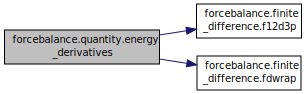
\includegraphics[width=350pt]{namespaceforcebalance_1_1quantity_a7968a8de12ab0744963598c488f91a4d_cgraph}
\end{center}
\end{figure}


\hypertarget{namespaceforcebalance_1_1quantity_a22d7b6184a255d4053ed1b6936e576f3}{\index{forcebalance\-::quantity@{forcebalance\-::quantity}!mean\-\_\-stderr@{mean\-\_\-stderr}}
\index{mean\-\_\-stderr@{mean\-\_\-stderr}!forcebalance::quantity@{forcebalance\-::quantity}}
\paragraph[{mean\-\_\-stderr}]{\setlength{\rightskip}{0pt plus 5cm}def forcebalance.\-quantity.\-mean\-\_\-stderr (
\begin{DoxyParamCaption}
\item[{}]{ts}
\end{DoxyParamCaption}
)}}\label{namespaceforcebalance_1_1quantity_a22d7b6184a255d4053ed1b6936e576f3}


Return mean and standard deviation of a time series ts. 



Definition at line 17 of file quantity.\-py.



Here is the call graph for this function\-:
\nopagebreak
\begin{figure}[H]
\begin{center}
\leavevmode
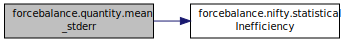
\includegraphics[width=350pt]{namespaceforcebalance_1_1quantity_a22d7b6184a255d4053ed1b6936e576f3_cgraph}
\end{center}
\end{figure}




\subsubsection{Variable Documentation}
\hypertarget{namespaceforcebalance_1_1quantity_a1d4f48df65583ff66457beb51ef5c361}{\index{forcebalance\-::quantity@{forcebalance\-::quantity}!logger@{logger}}
\index{logger@{logger}!forcebalance::quantity@{forcebalance\-::quantity}}
\paragraph[{logger}]{\setlength{\rightskip}{0pt plus 5cm}tuple forcebalance.\-quantity.\-logger = get\-Logger(\-\_\-\-\_\-name\-\_\-\-\_\-)}}\label{namespaceforcebalance_1_1quantity_a1d4f48df65583ff66457beb51ef5c361}


Definition at line 12 of file quantity.\-py.


\hypertarget{namespaceforcebalance_1_1target}{\subsection{forcebalance.\-target Namespace Reference}
\label{namespaceforcebalance_1_1target}\index{forcebalance.\-target@{forcebalance.\-target}}
}
\subsubsection*{Classes}
\begin{DoxyCompactItemize}
\item 
class \hyperlink{classforcebalance_1_1target_1_1Target}{Target}
\begin{DoxyCompactList}\small\item\em Base class for all fitting targets. \end{DoxyCompactList}\end{DoxyCompactItemize}
\subsubsection*{Variables}
\begin{DoxyCompactItemize}
\item 
tuple \hyperlink{namespaceforcebalance_1_1target_a976b578b7936f7ef8f929a98f3979bd7}{logger} = get\-Logger(\-\_\-\-\_\-name\-\_\-\-\_\-)
\end{DoxyCompactItemize}


\subsubsection{Variable Documentation}
\hypertarget{namespaceforcebalance_1_1target_a976b578b7936f7ef8f929a98f3979bd7}{\index{forcebalance\-::target@{forcebalance\-::target}!logger@{logger}}
\index{logger@{logger}!forcebalance::target@{forcebalance\-::target}}
\paragraph[{logger}]{\setlength{\rightskip}{0pt plus 5cm}tuple forcebalance.\-target.\-logger = get\-Logger(\-\_\-\-\_\-name\-\_\-\-\_\-)}}\label{namespaceforcebalance_1_1target_a976b578b7936f7ef8f929a98f3979bd7}


Definition at line 16 of file target.\-py.


\hypertarget{namespaceforcebalance_1_1thermo}{\subsection{forcebalance.\-thermo Namespace Reference}
\label{namespaceforcebalance_1_1thermo}\index{forcebalance.\-thermo@{forcebalance.\-thermo}}
}
\subsubsection*{Classes}
\begin{DoxyCompactItemize}
\item 
class \hyperlink{classforcebalance_1_1thermo_1_1Thermo}{Thermo}
\begin{DoxyCompactList}\small\item\em A target for fitting general experimental data sets. \end{DoxyCompactList}\item 
class \hyperlink{classforcebalance_1_1thermo_1_1Point}{Point}
\end{DoxyCompactItemize}
\subsubsection*{Variables}
\begin{DoxyCompactItemize}
\item 
tuple \hyperlink{namespaceforcebalance_1_1thermo_ae82b6b46a271d5e703659d175cf81632}{logger} = get\-Logger(\-\_\-\-\_\-name\-\_\-\-\_\-)
\end{DoxyCompactItemize}


\subsubsection{Variable Documentation}
\hypertarget{namespaceforcebalance_1_1thermo_ae82b6b46a271d5e703659d175cf81632}{\index{forcebalance\-::thermo@{forcebalance\-::thermo}!logger@{logger}}
\index{logger@{logger}!forcebalance::thermo@{forcebalance\-::thermo}}
\paragraph[{logger}]{\setlength{\rightskip}{0pt plus 5cm}tuple forcebalance.\-thermo.\-logger = get\-Logger(\-\_\-\-\_\-name\-\_\-\-\_\-)}}\label{namespaceforcebalance_1_1thermo_ae82b6b46a271d5e703659d175cf81632}


Definition at line 15 of file thermo.\-py.


\hypertarget{namespaceforcebalance_1_1tinkerio}{}\subsection{forcebalance.\+tinkerio Namespace Reference}
\label{namespaceforcebalance_1_1tinkerio}\index{forcebalance.\+tinkerio@{forcebalance.\+tinkerio}}


T\+I\+N\+K\+ER input/output.  




\subsubsection{Detailed Description}
T\+I\+N\+K\+ER input/output. 

This serves as a good template for writing future force matching I/O modules for other programs because it\textquotesingle{}s so simple.

\begin{DoxyAuthor}{Author}
Lee-\/\+Ping Wang 
\end{DoxyAuthor}
\begin{DoxyDate}{Date}
01/2012 
\end{DoxyDate}

\hypertarget{namespaceforcebalance_1_1vibration}{\subsection{forcebalance.\-vibration Namespace Reference}
\label{namespaceforcebalance_1_1vibration}\index{forcebalance.\-vibration@{forcebalance.\-vibration}}
}


Vibrational mode fitting module.  


\subsubsection*{Classes}
\begin{DoxyCompactItemize}
\item 
class \hyperlink{classforcebalance_1_1vibration_1_1Vibration}{Vibration}
\begin{DoxyCompactList}\small\item\em Subclass of Target for fitting force fields to vibrational spectra (from experiment or theory). \end{DoxyCompactList}\end{DoxyCompactItemize}
\subsubsection*{Functions}
\begin{DoxyCompactItemize}
\item 
def \hyperlink{namespaceforcebalance_1_1vibration_aaecc1b522065d7db7c68ca030ab7c449}{count\-\_\-assignment}
\end{DoxyCompactItemize}
\subsubsection*{Variables}
\begin{DoxyCompactItemize}
\item 
tuple \hyperlink{namespaceforcebalance_1_1vibration_a1aaf46e8f2b2c8eedf65477360094c0b}{logger} = get\-Logger(\-\_\-\-\_\-name\-\_\-\-\_\-)
\end{DoxyCompactItemize}


\subsubsection{Detailed Description}
Vibrational mode fitting module. \begin{DoxyAuthor}{Author}
Lee-\/\-Ping Wang 
\end{DoxyAuthor}
\begin{DoxyDate}{Date}
08/2012 
\end{DoxyDate}


\subsubsection{Function Documentation}
\hypertarget{namespaceforcebalance_1_1vibration_aaecc1b522065d7db7c68ca030ab7c449}{\index{forcebalance\-::vibration@{forcebalance\-::vibration}!count\-\_\-assignment@{count\-\_\-assignment}}
\index{count\-\_\-assignment@{count\-\_\-assignment}!forcebalance::vibration@{forcebalance\-::vibration}}
\paragraph[{count\-\_\-assignment}]{\setlength{\rightskip}{0pt plus 5cm}def forcebalance.\-vibration.\-count\-\_\-assignment (
\begin{DoxyParamCaption}
\item[{}]{assignment, }
\item[{}]{verbose = {\ttfamily True}}
\end{DoxyParamCaption}
)}}\label{namespaceforcebalance_1_1vibration_aaecc1b522065d7db7c68ca030ab7c449}


Definition at line 25 of file vibration.\-py.



\subsubsection{Variable Documentation}
\hypertarget{namespaceforcebalance_1_1vibration_a1aaf46e8f2b2c8eedf65477360094c0b}{\index{forcebalance\-::vibration@{forcebalance\-::vibration}!logger@{logger}}
\index{logger@{logger}!forcebalance::vibration@{forcebalance\-::vibration}}
\paragraph[{logger}]{\setlength{\rightskip}{0pt plus 5cm}tuple forcebalance.\-vibration.\-logger = get\-Logger(\-\_\-\-\_\-name\-\_\-\-\_\-)}}\label{namespaceforcebalance_1_1vibration_a1aaf46e8f2b2c8eedf65477360094c0b}


Definition at line 23 of file vibration.\-py.


\section{File Documentation}
\hypertarget{____init_____8py}{\subsection{\-\_\-\-\_\-init\-\_\-\-\_\-.\-py File Reference}
\label{____init_____8py}\index{\-\_\-\-\_\-init\-\_\-\-\_\-.\-py@{\-\_\-\-\_\-init\-\_\-\-\_\-.\-py}}
}
\subsubsection*{Classes}
\begin{DoxyCompactItemize}
\item 
class \hyperlink{classforcebalance_1_1BaseClass}{forcebalance.\-Base\-Class}
\begin{DoxyCompactList}\small\item\em Provides some nifty functions that are common to all Force\-Balance classes. \end{DoxyCompactList}\item 
class \hyperlink{classforcebalance_1_1BaseReader}{forcebalance.\-Base\-Reader}
\begin{DoxyCompactList}\small\item\em The 'reader' class. \end{DoxyCompactList}\end{DoxyCompactItemize}
\subsubsection*{Namespaces}
\begin{DoxyCompactItemize}
\item 
\hyperlink{namespaceforcebalance}{forcebalance}
\end{DoxyCompactItemize}
\subsubsection*{Variables}
\begin{DoxyCompactItemize}
\item 
tuple \hyperlink{namespaceforcebalance_a6c10581ea309550b5703fbe56f62e8a2}{forcebalance.\-\_\-\-\_\-version\-\_\-\-\_\-} = pkg\-\_\-resources.\-get\-\_\-distribution(\char`\"{}forcebalance\char`\"{})
\end{DoxyCompactItemize}

\hypertarget{abinitio_8py}{}\subsection{abinitio.\+py File Reference}
\label{abinitio_8py}\index{abinitio.\+py@{abinitio.\+py}}
\subsubsection*{Classes}
\begin{DoxyCompactItemize}
\item 
class \hyperlink{classsrc_1_1abinitio_1_1AbInitio}{src.\+abinitio.\+Ab\+Initio}
\begin{DoxyCompactList}\small\item\em Subclass of Target for fitting force fields to ab initio data. \end{DoxyCompactList}\end{DoxyCompactItemize}
\subsubsection*{Namespaces}
\begin{DoxyCompactItemize}
\item 
 \hyperlink{namespacesrc_1_1abinitio}{src.\+abinitio}
\item 
 \hyperlink{namespaceforcebalance_1_1abinitio}{forcebalance.\+abinitio}
\begin{DoxyCompactList}\small\item\em Ab-\/initio fitting module (energies, forces, resp). \end{DoxyCompactList}\end{DoxyCompactItemize}
\subsubsection*{Functions}
\begin{DoxyCompactItemize}
\item 
def \hyperlink{namespacesrc_1_1abinitio_ae5e4372a8a2b6ae643c954f1717761a5}{src.\+abinitio.\+norm2} (arr, a=0, n=None, step=3)
\begin{DoxyCompactList}\small\item\em Given a one-\/dimensional array, return the norm-\/squared of every \char`\"{}step\char`\"{} elements, starting at \textquotesingle{}a\textquotesingle{} and computing \textquotesingle{}n\textquotesingle{} total elements (so arr\mbox{[}a\+:a+step$\ast$n\mbox{]} must be valid). \end{DoxyCompactList}\item 
def \hyperlink{namespacesrc_1_1abinitio_ace4aca44aab54100556205a5aeab3cad}{src.\+abinitio.\+compute\+\_\+objective\+\_\+part} (S\+PX, Q\+Q0, Q0, Z, a, n, energy=False, subtract\+\_\+mean=False, divide=1, L=None, R=None, L2=None, R2=None)
\item 
def \hyperlink{namespacesrc_1_1abinitio_a15ff594ec7734a01ef603b9bb780d966}{src.\+abinitio.\+plot\+\_\+qm\+\_\+vs\+\_\+mm} (Q, M, M\+\_\+orig=None, title=\textquotesingle{}\textquotesingle{})
\end{DoxyCompactItemize}
\subsubsection*{Variables}
\begin{DoxyCompactItemize}
\item 
\hyperlink{namespacesrc_1_1abinitio_a5f31a5792044a3fac63afc0cf112ac9c}{src.\+abinitio.\+logger} = get\+Logger(\+\_\+\+\_\+name\+\_\+\+\_\+)
\end{DoxyCompactItemize}

\hypertarget{abinitio__internal_8py}{\subsection{abinitio\-\_\-internal.\-py File Reference}
\label{abinitio__internal_8py}\index{abinitio\-\_\-internal.\-py@{abinitio\-\_\-internal.\-py}}
}
\subsubsection*{Namespaces}
\begin{DoxyCompactItemize}
\item 
\hyperlink{namespaceforcebalance_1_1abinitio__internal}{forcebalance.\-abinitio\-\_\-internal}
\end{DoxyCompactItemize}

\hypertarget{amberio_8py}{\subsection{amberio.\-py File Reference}
\label{amberio_8py}\index{amberio.\-py@{amberio.\-py}}
}
\subsubsection*{Namespaces}
\begin{DoxyCompactItemize}
\item 
\hyperlink{namespaceforcebalance_1_1amberio}{forcebalance.\-amberio}
\end{DoxyCompactItemize}

\hypertarget{api_8dox}{}\subsection{api.\+dox File Reference}
\label{api_8dox}\index{api.\+dox@{api.\+dox}}

\hypertarget{binding_8py}{\subsection{binding.\-py File Reference}
\label{binding_8py}\index{binding.\-py@{binding.\-py}}
}
\subsubsection*{Namespaces}
\begin{DoxyCompactItemize}
\item 
\hyperlink{namespaceforcebalance_1_1binding}{forcebalance.\-binding}
\end{DoxyCompactItemize}

\hypertarget{chemistry_8py}{\subsection{chemistry.\-py \-File \-Reference}
\label{chemistry_8py}\index{chemistry.\-py@{chemistry.\-py}}
}
\subsubsection*{\-Packages}
\begin{DoxyCompactItemize}
\item 
namespace \hyperlink{namespaceforcebalance_1_1chemistry}{forcebalance\-::chemistry}
\end{DoxyCompactItemize}
\subsubsection*{\-Functions}
\begin{DoxyCompactItemize}
\item 
def \hyperlink{namespaceforcebalance_1_1chemistry_a7f1904563d4cc7623dcc4fdab5c645a0}{forcebalance\-::chemistry.\-Lookup\-By\-Mass}
\item 
def \hyperlink{namespaceforcebalance_1_1chemistry_a843280e0ccfc3059271008be88b38a42}{forcebalance\-::chemistry.\-Bond\-Strength\-By\-Length}
\end{DoxyCompactItemize}
\subsubsection*{\-Variables}
\begin{DoxyCompactItemize}
\item 
tuple \hyperlink{namespaceforcebalance_1_1chemistry_aa32672abf21f3992401f7869fef4b579}{forcebalance\-::chemistry.\-Bond\-Energies} = defaultdict(lambda\-:defaultdict(dict))
\item 
list \hyperlink{namespaceforcebalance_1_1chemistry_a5db7a023d3980e17137379852d5c8551}{forcebalance\-::chemistry.\-Radii}
\begin{DoxyCompactList}\small\item\em \-Covalent radii from \-Cordero et al. \end{DoxyCompactList}\item 
dictionary \hyperlink{namespaceforcebalance_1_1chemistry_a10486086db3bcc2c63c591c726b3464f}{forcebalance\-::chemistry.\-Periodic\-Table}
\item 
list \hyperlink{namespaceforcebalance_1_1chemistry_a12ef5f22f5cc3798107d3585c77a1c84}{forcebalance\-::chemistry.\-Elements}
\item 
list \hyperlink{namespaceforcebalance_1_1chemistry_a70b1983d2e59ef37617b0a80a3fd14c9}{forcebalance\-::chemistry.\-Bond\-Chars} = \mbox{[}'-\/','=','3'\mbox{]}
\item 
string \hyperlink{namespaceforcebalance_1_1chemistry_a244dd58baf4c171b37316e64561c1021}{forcebalance\-::chemistry.\-data\-\_\-from\-\_\-web}
\item 
tuple \hyperlink{namespaceforcebalance_1_1chemistry_a43d08c70d93e430fc6fd6689f622b61b}{forcebalance\-::chemistry.\-line} = line.\-expandtabs()
\item 
tuple \hyperlink{namespaceforcebalance_1_1chemistry_a2e8b0b69254f9a7346919dc00f606e74}{forcebalance\-::chemistry.\-B\-E} = float(line.\-split()\mbox{[}1\mbox{]})
\item 
tuple \hyperlink{namespaceforcebalance_1_1chemistry_ace6400fcf0f12a9d9f70aa7496984379}{forcebalance\-::chemistry.\-L} = float(line.\-split()\mbox{[}2\mbox{]})
\item 
tuple \hyperlink{namespaceforcebalance_1_1chemistry_a769e0e6c4bad669c6786d1ff12354978}{forcebalance\-::chemistry.\-atoms} = re.\-split('\mbox{[}-\/=3\mbox{]}', line.\-split()\mbox{[}0\mbox{]})
\item 
list \hyperlink{namespaceforcebalance_1_1chemistry_a4f490f29c23b8f185dc926e38eb7e746}{forcebalance\-::chemistry.\-A} = atoms\mbox{[}0\mbox{]}
\item 
list \hyperlink{namespaceforcebalance_1_1chemistry_a408afe99c28b09783c769307b8819f78}{forcebalance\-::chemistry.\-B} = atoms\mbox{[}1\mbox{]}
\item 
tuple \hyperlink{namespaceforcebalance_1_1chemistry_a1ef8f483a40113a668ff3743bb56d7ad}{forcebalance\-::chemistry.\-bo} = \-Bond\-Chars.\-index(re.\-findall('\mbox{[}-\/=3\mbox{]}', line.\-split()\mbox{[}0\mbox{]})\mbox{[}0\mbox{]})
\end{DoxyCompactItemize}

\hypertarget{contact_8py}{\subsection{contact.\-py File Reference}
\label{contact_8py}\index{contact.\-py@{contact.\-py}}
}
\subsubsection*{Namespaces}
\begin{DoxyCompactItemize}
\item 
\hyperlink{namespaceforcebalance_1_1contact}{forcebalance.\-contact}
\end{DoxyCompactItemize}
\subsubsection*{Functions}
\begin{DoxyCompactItemize}
\item 
def \hyperlink{namespaceforcebalance_1_1contact_a3592dbbf524c6115f34d9a70b50e2e0f}{forcebalance.\-contact.\-atom\-\_\-distances}
\begin{DoxyCompactList}\small\item\em For each frame in xyzlist, compute the (euclidean) distance between pairs of atoms whos indices are given in contacts. \end{DoxyCompactList}\item 
def \hyperlink{namespaceforcebalance_1_1contact_acffb04a66580454b8a87648faa1c5c16}{forcebalance.\-contact.\-residue\-\_\-distances}
\begin{DoxyCompactList}\small\item\em For each frame in xyzlist, and for each pair of residues in the array contact, compute the distance between the closest pair of atoms such that one of them belongs to each residue. \end{DoxyCompactList}\end{DoxyCompactItemize}

\hypertarget{counterpoise_8py}{\subsection{counterpoise.\-py \-File \-Reference}
\label{counterpoise_8py}\index{counterpoise.\-py@{counterpoise.\-py}}
}
\subsubsection*{\-Classes}
\begin{DoxyCompactItemize}
\item 
class \hyperlink{classforcebalance_1_1counterpoise_1_1Counterpoise}{forcebalance.\-counterpoise.\-Counterpoise}
\begin{DoxyCompactList}\small\item\em \-Target subclass for matching the counterpoise correction. \end{DoxyCompactList}\end{DoxyCompactItemize}
\subsubsection*{\-Packages}
\begin{DoxyCompactItemize}
\item 
namespace \hyperlink{namespaceforcebalance_1_1counterpoise}{forcebalance\-::counterpoise}
\begin{DoxyCompactList}\small\item\em \-Match an empirical potential to the counterpoise correction for basis set superposition error (\-B\-S\-S\-E). \end{DoxyCompactList}\end{DoxyCompactItemize}
\subsubsection*{\-Variables}
\begin{DoxyCompactItemize}
\item 
tuple \hyperlink{namespaceforcebalance_1_1counterpoise_a5a5391fb65604f4aeba9c2e39557b547}{forcebalance\-::counterpoise.\-logger} = get\-Logger(\-\_\-\-\_\-name\-\_\-\-\_\-)
\end{DoxyCompactItemize}

\hypertarget{custom__io_8py}{\subsection{custom\-\_\-io.\-py File Reference}
\label{custom__io_8py}\index{custom\-\_\-io.\-py@{custom\-\_\-io.\-py}}
}
\subsubsection*{Namespaces}
\begin{DoxyCompactItemize}
\item 
\hyperlink{namespaceforcebalance_1_1custom__io}{forcebalance.\-custom\-\_\-io}
\end{DoxyCompactItemize}

\hypertarget{engine_8py}{\subsection{engine.\-py File Reference}
\label{engine_8py}\index{engine.\-py@{engine.\-py}}
}
\subsubsection*{Classes}
\begin{DoxyCompactItemize}
\item 
class \hyperlink{classforcebalance_1_1engine_1_1Engine}{forcebalance.\-engine.\-Engine}
\begin{DoxyCompactList}\small\item\em Base class for all engines. \end{DoxyCompactList}\end{DoxyCompactItemize}
\subsubsection*{Namespaces}
\begin{DoxyCompactItemize}
\item 
\hyperlink{namespaceforcebalance_1_1engine}{forcebalance.\-engine}
\end{DoxyCompactItemize}
\subsubsection*{Variables}
\begin{DoxyCompactItemize}
\item 
tuple \hyperlink{namespaceforcebalance_1_1engine_ae9028cb0bf779c6a559e168e15e7ace1}{forcebalance.\-engine.\-logger} = get\-Logger(\-\_\-\-\_\-name\-\_\-\-\_\-)
\end{DoxyCompactItemize}

\hypertarget{finite__difference_8py}{\subsection{finite\-\_\-difference.\-py File Reference}
\label{finite__difference_8py}\index{finite\-\_\-difference.\-py@{finite\-\_\-difference.\-py}}
}
\subsubsection*{Namespaces}
\begin{DoxyCompactItemize}
\item 
\hyperlink{namespaceforcebalance_1_1finite__difference}{forcebalance.\-finite\-\_\-difference}
\end{DoxyCompactItemize}
\subsubsection*{Functions}
\begin{DoxyCompactItemize}
\item 
def \hyperlink{namespaceforcebalance_1_1finite__difference_ac5bb1552a9b8dd22c9c80e6444de2218}{forcebalance.\-finite\-\_\-difference.\-f1d2p}
\begin{DoxyCompactList}\small\item\em A two-\/point finite difference stencil. \end{DoxyCompactList}\item 
def \hyperlink{namespaceforcebalance_1_1finite__difference_a123c5d5dea0f3f50ab57796bb3bc39be}{forcebalance.\-finite\-\_\-difference.\-f1d5p}
\begin{DoxyCompactList}\small\item\em A highly accurate five-\/point finite difference stencil for computing derivatives of a function. \end{DoxyCompactList}\item 
def \hyperlink{namespaceforcebalance_1_1finite__difference_a9be9f0d21300958092e380514e2e980d}{forcebalance.\-finite\-\_\-difference.\-f1d7p}
\begin{DoxyCompactList}\small\item\em A highly accurate seven-\/point finite difference stencil for computing derivatives of a function. \end{DoxyCompactList}\item 
def \hyperlink{namespaceforcebalance_1_1finite__difference_acc281f85b668062745f711d9b4a610fa}{forcebalance.\-finite\-\_\-difference.\-f12d7p}
\item 
def \hyperlink{namespaceforcebalance_1_1finite__difference_aa69a8819e4680091f400303c1d6ddeb7}{forcebalance.\-finite\-\_\-difference.\-f12d3p}
\begin{DoxyCompactList}\small\item\em A three-\/point finite difference stencil. \end{DoxyCompactList}\item 
def \hyperlink{namespaceforcebalance_1_1finite__difference_a25b9b661eb48d97d7ded70f4ccf50bbb}{forcebalance.\-finite\-\_\-difference.\-f2var}
\begin{DoxyCompactList}\small\item\em A finite difference stencil for a function of two variables. \end{DoxyCompactList}\item 
def \hyperlink{namespaceforcebalance_1_1finite__difference_ad84d3e385db1190e7d8ef58bc08a6c52}{forcebalance.\-finite\-\_\-difference.\-in\-\_\-fd}
\begin{DoxyCompactList}\small\item\em Invoking this function from anywhere will tell us whether we're being called by a finite-\/difference function. \end{DoxyCompactList}\item 
def \hyperlink{namespaceforcebalance_1_1finite__difference_a978c262bfab74a29143808b7562ab61b}{forcebalance.\-finite\-\_\-difference.\-in\-\_\-fd\-\_\-srch}
\begin{DoxyCompactList}\small\item\em Invoking this function from anywhere will tell us whether we're being called by a finite-\/difference function. \end{DoxyCompactList}\item 
def \hyperlink{namespaceforcebalance_1_1finite__difference_ae484c591ae8c4e5bae73a0ef2660c339}{forcebalance.\-finite\-\_\-difference.\-fdwrap}
\begin{DoxyCompactList}\small\item\em A function wrapper for finite difference designed for differentiating 'get'-\/type functions. \end{DoxyCompactList}\item 
def \hyperlink{namespaceforcebalance_1_1finite__difference_a00322fb65860c390616f74d05037c797}{forcebalance.\-finite\-\_\-difference.\-fdwrap\-\_\-\-G}
\begin{DoxyCompactList}\small\item\em A driver to fdwrap for gradients (see documentation for fdwrap) Inputs\-: tgt = The Target containing the objective function that we want to differentiate mvals0 = The 'central' values of the mathematical parameters -\/ i.\-e. \end{DoxyCompactList}\item 
def \hyperlink{namespaceforcebalance_1_1finite__difference_a77a0bc1ae3cbbcc8d38a0ef9ca877d6d}{forcebalance.\-finite\-\_\-difference.\-fdwrap\-\_\-\-H}
\begin{DoxyCompactList}\small\item\em A driver to fdwrap for Hessians (see documentation for fdwrap) Inputs\-: tgt = The Target containing the objective function that we want to differentiate mvals0 = The 'central' values of the mathematical parameters -\/ i.\-e. \end{DoxyCompactList}\end{DoxyCompactItemize}
\subsubsection*{Variables}
\begin{DoxyCompactItemize}
\item 
tuple \hyperlink{namespaceforcebalance_1_1finite__difference_a2bdf74505c45f442e1c96d557414254e}{forcebalance.\-finite\-\_\-difference.\-logger} = get\-Logger(\-\_\-\-\_\-name\-\_\-\-\_\-)
\end{DoxyCompactItemize}

\hypertarget{forcefield_8py}{\subsection{forcefield.\-py File Reference}
\label{forcefield_8py}\index{forcefield.\-py@{forcefield.\-py}}
}
\subsubsection*{Classes}
\begin{DoxyCompactItemize}
\item 
class \hyperlink{classforcebalance_1_1forcefield_1_1BackedUpDict}{forcebalance.\-forcefield.\-Backed\-Up\-Dict}
\item 
class \hyperlink{classforcebalance_1_1forcefield_1_1FF}{forcebalance.\-forcefield.\-F\-F}
\begin{DoxyCompactList}\small\item\em Force field class. \end{DoxyCompactList}\end{DoxyCompactItemize}
\subsubsection*{Namespaces}
\begin{DoxyCompactItemize}
\item 
namespace \hyperlink{namespaceforcebalance_1_1forcefield}{forcebalance.\-forcefield}
\begin{DoxyCompactList}\small\item\em Force field module. \end{DoxyCompactList}\end{DoxyCompactItemize}
\subsubsection*{Functions}
\begin{DoxyCompactItemize}
\item 
def \hyperlink{namespaceforcebalance_1_1forcefield_a99c9997d5158a04be089f291bd6f99bd}{forcebalance.\-forcefield.\-determine\-\_\-fftype}
\begin{DoxyCompactList}\small\item\em Determine the type of a force field file. \end{DoxyCompactList}\item 
def \hyperlink{namespaceforcebalance_1_1forcefield_ab1a855bace20dd5e45928467e2a133f1}{forcebalance.\-forcefield.\-rs\-\_\-override}
\begin{DoxyCompactList}\small\item\em This function takes in a dictionary (rsfactors) and a string (termtype). \end{DoxyCompactList}\end{DoxyCompactItemize}
\subsubsection*{Variables}
\begin{DoxyCompactItemize}
\item 
tuple \hyperlink{namespaceforcebalance_1_1forcefield_ab770be419e9b4522779dc3dfb1d7d019}{forcebalance.\-forcefield.\-logger} = get\-Logger(\-\_\-\-\_\-name\-\_\-\-\_\-)
\item 
dictionary \hyperlink{namespaceforcebalance_1_1forcefield_abc5e12aa78c5742f028b954ede086c51}{forcebalance.\-forcefield.\-F\-F\-\_\-\-Extensions}
\item 
dictionary \hyperlink{namespaceforcebalance_1_1forcefield_a3beac9806e0438b79b9ae60a47c7b131}{forcebalance.\-forcefield.\-F\-F\-\_\-\-I\-O\-Modules}
\end{DoxyCompactItemize}

\hypertarget{gmxio_8py}{\subsection{gmxio.\-py File Reference}
\label{gmxio_8py}\index{gmxio.\-py@{gmxio.\-py}}
}
\subsubsection*{Namespaces}
\begin{DoxyCompactItemize}
\item 
\hyperlink{namespaceforcebalance_1_1gmxio}{forcebalance.\-gmxio}
\end{DoxyCompactItemize}

\hypertarget{interaction_8py}{\subsection{interaction.\-py File Reference}
\label{interaction_8py}\index{interaction.\-py@{interaction.\-py}}
}
\subsubsection*{Classes}
\begin{DoxyCompactItemize}
\item 
class \hyperlink{classforcebalance_1_1interaction_1_1Interaction}{forcebalance.\-interaction.\-Interaction}
\begin{DoxyCompactList}\small\item\em Subclass of Target for fitting force fields to interaction energies. \end{DoxyCompactList}\end{DoxyCompactItemize}
\subsubsection*{Namespaces}
\begin{DoxyCompactItemize}
\item 
namespace \hyperlink{namespaceforcebalance_1_1interaction}{forcebalance.\-interaction}
\begin{DoxyCompactList}\small\item\em \hyperlink{classforcebalance_1_1interaction_1_1Interaction}{Interaction} energy fitting module. \end{DoxyCompactList}\end{DoxyCompactItemize}

\hypertarget{leastsq_8py}{\subsection{leastsq.\-py File Reference}
\label{leastsq_8py}\index{leastsq.\-py@{leastsq.\-py}}
}
\subsubsection*{Classes}
\begin{DoxyCompactItemize}
\item 
class \hyperlink{classforcebalance_1_1leastsq_1_1LeastSquares}{forcebalance.\-leastsq.\-Least\-Squares}
\begin{DoxyCompactList}\small\item\em Subclass of Target for general least squares fitting. \end{DoxyCompactList}\end{DoxyCompactItemize}
\subsubsection*{Namespaces}
\begin{DoxyCompactItemize}
\item 
namespace \hyperlink{namespaceforcebalance_1_1leastsq}{forcebalance.\-leastsq}
\item 
namespace \hyperlink{namespaceforcebalance_1_1abinitio}{forcebalance.\-abinitio}
\begin{DoxyCompactList}\small\item\em Ab-\/initio fitting module (energies, forces, resp). \end{DoxyCompactList}\end{DoxyCompactItemize}
\subsubsection*{Functions}
\begin{DoxyCompactItemize}
\item 
def \hyperlink{namespaceforcebalance_1_1leastsq_a8e7ef329e27aff738bc91dd79bd2dd1c}{forcebalance.\-leastsq.\-Check\-Basis}
\item 
def \hyperlink{namespaceforcebalance_1_1leastsq_ad9d0036b0003e0245608ffb192c7c60c}{forcebalance.\-leastsq.\-Last\-Mvals}
\end{DoxyCompactItemize}
\subsubsection*{Variables}
\begin{DoxyCompactItemize}
\item 
tuple \hyperlink{namespaceforcebalance_1_1leastsq_ab5873c70f3da934d9c5c78ca9c7ca8d0}{forcebalance.\-leastsq.\-logger} = get\-Logger(\-\_\-\-\_\-name\-\_\-\-\_\-)
\item 
\hyperlink{namespaceforcebalance_1_1leastsq_a87815b7768ddc6d9caf7fa3c804fe303}{forcebalance.\-leastsq.\-C\-H\-E\-C\-K\-\_\-\-B\-A\-S\-I\-S} = False
\item 
\hyperlink{namespaceforcebalance_1_1leastsq_a037a62063d126288c2df0f4e0cd5085a}{forcebalance.\-leastsq.\-L\-A\-S\-T\-\_\-\-M\-V\-A\-L\-S} = None
\end{DoxyCompactItemize}

\hypertarget{lipid_8py}{\subsection{lipid.\-py File Reference}
\label{lipid_8py}\index{lipid.\-py@{lipid.\-py}}
}
\subsubsection*{Namespaces}
\begin{DoxyCompactItemize}
\item 
\hyperlink{namespaceforcebalance_1_1lipid}{forcebalance.\-lipid}
\end{DoxyCompactItemize}

\hypertarget{liquid_8py}{}\subsection{liquid.\+py File Reference}
\label{liquid_8py}\index{liquid.\+py@{liquid.\+py}}
\subsubsection*{Classes}
\begin{DoxyCompactItemize}
\item 
class \hyperlink{classsrc_1_1liquid_1_1Liquid}{src.\+liquid.\+Liquid}
\begin{DoxyCompactList}\small\item\em Subclass of Target for liquid property matching. \end{DoxyCompactList}\end{DoxyCompactItemize}
\subsubsection*{Namespaces}
\begin{DoxyCompactItemize}
\item 
 \hyperlink{namespacesrc_1_1liquid}{src.\+liquid}
\item 
 \hyperlink{namespaceforcebalance_1_1liquid}{forcebalance.\+liquid}
\begin{DoxyCompactList}\small\item\em Matching of liquid bulk properties. \end{DoxyCompactList}\end{DoxyCompactItemize}
\subsubsection*{Functions}
\begin{DoxyCompactItemize}
\item 
def \hyperlink{namespacesrc_1_1liquid_a5ad9c3640a1f3ba97408b8ece94eb7c0}{src.\+liquid.\+weight\+\_\+info} (W, PT, N\+\_\+k, verbose=True, P\+TS=None)
\end{DoxyCompactItemize}
\subsubsection*{Variables}
\begin{DoxyCompactItemize}
\item 
\hyperlink{namespacesrc_1_1liquid_a94b65ba658e49a2161816eab3db1b1b6}{src.\+liquid.\+logger} = get\+Logger(\+\_\+\+\_\+name\+\_\+\+\_\+)
\end{DoxyCompactItemize}

\hypertarget{Mol2_8py}{\subsection{\-Mol2.\-py \-File \-Reference}
\label{Mol2_8py}\index{\-Mol2.\-py@{\-Mol2.\-py}}
}
\subsubsection*{\-Classes}
\begin{DoxyCompactItemize}
\item 
class \hyperlink{classforcebalance_1_1Mol2_1_1mol2__atom}{forcebalance.\-Mol2.\-mol2\-\_\-atom}
\begin{DoxyCompactList}\small\item\em \-This is to manage \hyperlink{classforcebalance_1_1Mol2_1_1mol2}{mol2} atomic lines on the form\-: 1 \-C1 5.\-4790 42.\-2880 49.\-5910 \-C.\-ar 1 $<$1$>$ 0.\-0424. \end{DoxyCompactList}\item 
class \hyperlink{classforcebalance_1_1Mol2_1_1mol2__bond}{forcebalance.\-Mol2.\-mol2\-\_\-bond}
\begin{DoxyCompactList}\small\item\em \-This is to manage \hyperlink{classforcebalance_1_1Mol2_1_1mol2}{mol2} bond lines on the form\-: 1 1 2 ar. \end{DoxyCompactList}\item 
class \hyperlink{classforcebalance_1_1Mol2_1_1mol2}{forcebalance.\-Mol2.\-mol2}
\begin{DoxyCompactList}\small\item\em \-This is to manage one \hyperlink{classforcebalance_1_1Mol2_1_1mol2}{mol2} series of lines on the form\-: \end{DoxyCompactList}\item 
class \hyperlink{classforcebalance_1_1Mol2_1_1mol2__set}{forcebalance.\-Mol2.\-mol2\-\_\-set}
\end{DoxyCompactItemize}
\subsubsection*{\-Packages}
\begin{DoxyCompactItemize}
\item 
namespace \hyperlink{namespaceforcebalance_1_1Mol2}{forcebalance\-::\-Mol2}
\end{DoxyCompactItemize}
\subsubsection*{\-Variables}
\begin{DoxyCompactItemize}
\item 
tuple \hyperlink{namespaceforcebalance_1_1Mol2_a41537283c77bf1c8e05a63667003ae1c}{forcebalance\-::\-Mol2.\-data} = mol2\-\_\-set(sys.\-argv\mbox{[}1\mbox{]}, subset=\mbox{[}\char`\"{}\-R\-N\-Ase.\-xray.\-inh8.\-1\-Q\-H\-C\char`\"{}\mbox{]})
\end{DoxyCompactItemize}

\hypertarget{mol2io_8py}{\subsection{mol2io.\-py File Reference}
\label{mol2io_8py}\index{mol2io.\-py@{mol2io.\-py}}
}
\subsubsection*{Namespaces}
\begin{DoxyCompactItemize}
\item 
\hyperlink{namespaceforcebalance_1_1mol2io}{forcebalance.\-mol2io}
\end{DoxyCompactItemize}

\hypertarget{molecule_8py}{\subsection{molecule.\-py File Reference}
\label{molecule_8py}\index{molecule.\-py@{molecule.\-py}}
}
\subsubsection*{Classes}
\begin{DoxyCompactItemize}
\item 
class \hyperlink{classforcebalance_1_1molecule_1_1MolfileTimestep}{forcebalance.\-molecule.\-Molfile\-Timestep}
\begin{DoxyCompactList}\small\item\em Wrapper for the timestep C structure used in molfile plugins. \end{DoxyCompactList}\item 
class \hyperlink{classforcebalance_1_1molecule_1_1Molecule}{forcebalance.\-molecule.\-Molecule}
\begin{DoxyCompactList}\small\item\em Lee-\/\-Ping's general file format conversion class. \end{DoxyCompactList}\end{DoxyCompactItemize}
\subsubsection*{Namespaces}
\begin{DoxyCompactItemize}
\item 
\hyperlink{namespaceforcebalance_1_1molecule}{forcebalance.\-molecule}
\end{DoxyCompactItemize}
\subsubsection*{Functions}
\begin{DoxyCompactItemize}
\item 
def \hyperlink{namespaceforcebalance_1_1molecule_af28de4693e5b8e82df900d0ac3c6c370}{forcebalance.\-molecule.\-get\-Element}
\item 
def \hyperlink{namespaceforcebalance_1_1molecule_a7429f0c377d6396711c128f6590ef810}{forcebalance.\-molecule.\-elem\-\_\-from\-\_\-atomname}
\begin{DoxyCompactList}\small\item\em Given an atom name, attempt to get the element in most cases. \end{DoxyCompactList}\item 
def \hyperlink{namespaceforcebalance_1_1molecule_ab8464fea13fad2a506792c2f1d7c93f3}{forcebalance.\-molecule.\-nodematch}
\item 
def \hyperlink{namespaceforcebalance_1_1molecule_a0dd31eff88d2bed0884ab21a13261d42}{forcebalance.\-molecule.\-isint}
\begin{DoxyCompactList}\small\item\em O\-N\-L\-Y matches integers! If you have a decimal point? None shall pass! \end{DoxyCompactList}\item 
def \hyperlink{namespaceforcebalance_1_1molecule_afe989ffd119568047fc8265b1d329a70}{forcebalance.\-molecule.\-isfloat}
\begin{DoxyCompactList}\small\item\em Matches A\-N\-Y number; it can be a decimal, scientific notation, integer, or what have you. \end{DoxyCompactList}\item 
def \hyperlink{namespaceforcebalance_1_1molecule_a0a6e3e79b04534bf2e83d09def189444}{forcebalance.\-molecule.\-Build\-Lattice\-From\-Lengths\-Angles}
\begin{DoxyCompactList}\small\item\em This function takes in three lattice lengths and three lattice angles, and tries to return a complete box specification. \end{DoxyCompactList}\item 
def \hyperlink{namespaceforcebalance_1_1molecule_a29fb1ac9324f4280f07c65baea339989}{forcebalance.\-molecule.\-Build\-Lattice\-From\-Vectors}
\begin{DoxyCompactList}\small\item\em This function takes in three lattice vectors and tries to return a complete box specification. \end{DoxyCompactList}\item 
def \hyperlink{namespaceforcebalance_1_1molecule_a2eba3cad44138b3b10ea883240888412}{forcebalance.\-molecule.\-format\-\_\-xyz\-\_\-coord}
\begin{DoxyCompactList}\small\item\em Print a line consisting of (element, x, y, z) in accordance with .xyz file format. \end{DoxyCompactList}\item 
def \hyperlink{namespaceforcebalance_1_1molecule_a41c13064e4285973aa6c49369d3d3390}{forcebalance.\-molecule.\-format\-\_\-gro\-\_\-coord}
\begin{DoxyCompactList}\small\item\em Print a line in accordance with .gro file format, with six decimal points of precision. \end{DoxyCompactList}\item 
def \hyperlink{namespaceforcebalance_1_1molecule_a4948e4662b8d2c8d515427d1bbb3d01e}{forcebalance.\-molecule.\-format\-\_\-xyzgen\-\_\-coord}
\begin{DoxyCompactList}\small\item\em Print a line consisting of (element, p, q, r, s, t, ...) where (p, q, r) are arbitrary atom-\/wise data (this might happen, for instance, with atomic charges) \end{DoxyCompactList}\item 
def \hyperlink{namespaceforcebalance_1_1molecule_ae25aa5331b3a2dd0e9d1e184380357db}{forcebalance.\-molecule.\-format\-\_\-gro\-\_\-box}
\begin{DoxyCompactList}\small\item\em Print a line corresponding to the box vector in accordance with .gro file format. \end{DoxyCompactList}\item 
def \hyperlink{namespaceforcebalance_1_1molecule_a12b7bb398c2fa49a223f258ec7737483}{forcebalance.\-molecule.\-is\-\_\-gro\-\_\-coord}
\begin{DoxyCompactList}\small\item\em Determines whether a line contains G\-R\-O\-M\-A\-C\-S data or not. \end{DoxyCompactList}\item 
def \hyperlink{namespaceforcebalance_1_1molecule_a838d85848bd817e801d0f5f6502217ef}{forcebalance.\-molecule.\-is\-\_\-charmm\-\_\-coord}
\begin{DoxyCompactList}\small\item\em Determines whether a line contains C\-H\-A\-R\-M\-M data or not. \end{DoxyCompactList}\item 
def \hyperlink{namespaceforcebalance_1_1molecule_aafc8c924eed4480fed8ddc9c474d3bc1}{forcebalance.\-molecule.\-is\-\_\-gro\-\_\-box}
\begin{DoxyCompactList}\small\item\em Determines whether a line contains a G\-R\-O\-M\-A\-C\-S box vector or not. \end{DoxyCompactList}\item 
def \hyperlink{namespaceforcebalance_1_1molecule_a4cdb2086978b281ed84cd66179c3f5b2}{forcebalance.\-molecule.\-add\-\_\-strip\-\_\-to\-\_\-mat}
\item 
def \hyperlink{namespaceforcebalance_1_1molecule_a58c3f09152db4d1c6e1db9df29c60c43}{forcebalance.\-molecule.\-pvec}
\item 
def \hyperlink{namespaceforcebalance_1_1molecule_a7fe52c2928c7b0329882541bef2e34cd}{forcebalance.\-molecule.\-grouper}
\begin{DoxyCompactList}\small\item\em Groups a big long iterable into groups of ten or what have you. \end{DoxyCompactList}\item 
def \hyperlink{namespaceforcebalance_1_1molecule_a5f529179461765fadbd0a742cdc2c677}{forcebalance.\-molecule.\-even\-\_\-list}
\begin{DoxyCompactList}\small\item\em Creates a list of number sequences divided as evenly as possible. \end{DoxyCompactList}\item 
def \hyperlink{namespaceforcebalance_1_1molecule_a5b50df23cc4d0e617fdc56538f0bea63}{forcebalance.\-molecule.\-both}
\item 
def \hyperlink{namespaceforcebalance_1_1molecule_a6f7c6217b1c64da309a8abd21dfdcf08}{forcebalance.\-molecule.\-diff}
\item 
def \hyperlink{namespaceforcebalance_1_1molecule_a75775be6563ad7f10695a9a45ff49ba9}{forcebalance.\-molecule.\-either}
\item 
def \hyperlink{namespaceforcebalance_1_1molecule_af02bf73765f34bbef81c4a5b000b86ce}{forcebalance.\-molecule.\-Euler\-Matrix}
\begin{DoxyCompactList}\small\item\em Constructs an Euler matrix from three Euler angles. \end{DoxyCompactList}\item 
def \hyperlink{namespaceforcebalance_1_1molecule_a8fcbb4a2b3470a85d25699b6f28a54fc}{forcebalance.\-molecule.\-Compute\-Overlap}
\begin{DoxyCompactList}\small\item\em Computes an 'overlap' between two molecules based on some fictitious density. \end{DoxyCompactList}\item 
def \hyperlink{namespaceforcebalance_1_1molecule_a9a58eb1746e51420f50da3f3a6d51485}{forcebalance.\-molecule.\-Align\-To\-Density}
\begin{DoxyCompactList}\small\item\em Computes a \char`\"{}overlap density\char`\"{} from two frames. \end{DoxyCompactList}\item 
def \hyperlink{namespaceforcebalance_1_1molecule_aa9ad9b92efa7bd3c1d589d62bbb8108e}{forcebalance.\-molecule.\-Align\-To\-Moments}
\begin{DoxyCompactList}\small\item\em Pre-\/aligns molecules to 'moment of inertia'. \end{DoxyCompactList}\item 
def \hyperlink{namespaceforcebalance_1_1molecule_a08840b73e95bf34bf9ca7ea36ad0492d}{forcebalance.\-molecule.\-get\-\_\-rotate\-\_\-translate}
\item 
def \hyperlink{namespaceforcebalance_1_1molecule_ae76fc5d05f43acc6006a4d1733818d71}{forcebalance.\-molecule.\-cartesian\-\_\-product2}
\begin{DoxyCompactList}\small\item\em Form a Cartesian product of two Num\-Py arrays. \end{DoxyCompactList}\item 
def \hyperlink{namespaceforcebalance_1_1molecule_ab9cb167fbbd809aedcf8c7434d405547}{forcebalance.\-molecule.\-main}
\end{DoxyCompactItemize}
\subsubsection*{Variables}
\begin{DoxyCompactItemize}
\item 
tuple \hyperlink{namespaceforcebalance_1_1molecule_a0044fa397e0923635a8b3e9625aa70f7}{forcebalance.\-molecule.\-Frame\-Variable\-Names}
\item 
tuple \hyperlink{namespaceforcebalance_1_1molecule_a5daa68e835dcb9877d6c3f2fb559b54b}{forcebalance.\-molecule.\-Atom\-Variable\-Names} = set(\mbox{[}'elem', 'partial\-\_\-charge', 'atomname', 'atomtype', 'tinkersuf', 'resid', 'resname', 'qcsuf', 'qm\-\_\-ghost', 'chain', 'altloc', 'icode'\mbox{]})
\item 
tuple \hyperlink{namespaceforcebalance_1_1molecule_a38e1c99e9567fe42b792af43db9b7488}{forcebalance.\-molecule.\-Meta\-Variable\-Names} = set(\mbox{[}'fnm', 'ftype', 'qcrems', 'qctemplate', 'charge', 'mult', 'bonds'\mbox{]})
\item 
tuple \hyperlink{namespaceforcebalance_1_1molecule_ab67efeab6049ec1f416b9ad1eed6ffcc}{forcebalance.\-molecule.\-Quantum\-Variable\-Names} = set(\mbox{[}'qcrems', 'qctemplate', 'charge', 'mult', 'qcsuf', 'qm\-\_\-ghost'\mbox{]})
\item 
\hyperlink{namespaceforcebalance_1_1molecule_a8fcfb88fe12a9256b61980f3d4fe3b63}{forcebalance.\-molecule.\-All\-Variable\-Names} = Quantum\-Variable\-Names$|$Atom\-Variable\-Names$|$Meta\-Variable\-Names$|$Frame\-Variable\-Names
\item 
list \hyperlink{namespaceforcebalance_1_1molecule_a74f55a89a14ca676b5a06441d1fdab19}{forcebalance.\-molecule.\-Radii}
\item 
list \hyperlink{namespaceforcebalance_1_1molecule_a1c99a11e8a749468698c9af6361a8a4c}{forcebalance.\-molecule.\-Elements}
\item 
tuple \hyperlink{namespaceforcebalance_1_1molecule_adc5040ec456762f2ac240fb08febbfdd}{forcebalance.\-molecule.\-Periodic\-Table}
\item 
float \hyperlink{namespaceforcebalance_1_1molecule_a76af9edfbaaa8999680e32aafe1b1b61}{forcebalance.\-molecule.\-bohrang} = 0.\-529177249
\begin{DoxyCompactList}\small\item\em One bohr equals this many angstroms. \end{DoxyCompactList}\item 
tuple \hyperlink{namespaceforcebalance_1_1molecule_a09d04113accea9c88b084051c5de29d1}{forcebalance.\-molecule.\-splitter} = re.\-compile(r'(\textbackslash{}s+$|$\textbackslash{}S+)')
\item 
tuple \hyperlink{namespaceforcebalance_1_1molecule_aa761cf1cf260e15d0b03a6f61569c840}{forcebalance.\-molecule.\-Box} = namedtuple('Box',\mbox{[}'a','b','c','alpha','beta','gamma','A','B','C','V'\mbox{]})
\item 
int \hyperlink{namespaceforcebalance_1_1molecule_a1ee5389ce8a9042e053c7972dbbfb005}{forcebalance.\-molecule.\-radian} = 180
\item 
\hyperlink{namespaceforcebalance_1_1molecule_a2986996d4f957928047df06fbec3717d}{forcebalance.\-molecule.\-Alive}
\end{DoxyCompactItemize}

\hypertarget{moments_8py}{\subsection{moments.\-py File Reference}
\label{moments_8py}\index{moments.\-py@{moments.\-py}}
}
\subsubsection*{Namespaces}
\begin{DoxyCompactItemize}
\item 
\hyperlink{namespaceforcebalance_1_1moments}{forcebalance.\-moments}
\end{DoxyCompactItemize}

\hypertarget{nifty_8py}{}\subsection{nifty.\+py File Reference}
\label{nifty_8py}\index{nifty.\+py@{nifty.\+py}}
\subsubsection*{Classes}
\begin{DoxyCompactItemize}
\item 
class \hyperlink{classsrc_1_1nifty_1_1RawStreamHandler}{src.\+nifty.\+Raw\+Stream\+Handler}
\begin{DoxyCompactList}\small\item\em Exactly like Stream\+Handler, except no newline character is printed at the end of each message. \end{DoxyCompactList}\item 
class \hyperlink{classsrc_1_1nifty_1_1RawFileHandler}{src.\+nifty.\+Raw\+File\+Handler}
\begin{DoxyCompactList}\small\item\em Exactly like File\+Handler, except no newline character is printed at the end of each message. \end{DoxyCompactList}\item 
class \hyperlink{classsrc_1_1nifty_1_1LineChunker}{src.\+nifty.\+Line\+Chunker}
\end{DoxyCompactItemize}
\subsubsection*{Namespaces}
\begin{DoxyCompactItemize}
\item 
 \hyperlink{namespacesrc_1_1nifty}{src.\+nifty}
\item 
 \hyperlink{namespaceforcebalance_1_1nifty}{forcebalance.\+nifty}
\begin{DoxyCompactList}\small\item\em Nifty functions, intended to be imported by any module within \hyperlink{namespaceForceBalance}{Force\+Balance}. \end{DoxyCompactList}\end{DoxyCompactItemize}
\subsubsection*{Functions}
\begin{DoxyCompactItemize}
\item 
def \hyperlink{namespacesrc_1_1nifty_a34440c957989ec79bedf20e097a9e196}{src.\+nifty.\+pvec1d} (vec1d, precision=1, format=\char`\"{}e\char`\"{}, loglevel=I\+N\+FO)
\begin{DoxyCompactList}\small\item\em Printout of a 1-\/D vector. \end{DoxyCompactList}\item 
def \hyperlink{namespacesrc_1_1nifty_ae6848e812afbae8005b70ed48087a1f2}{src.\+nifty.\+astr} (vec1d, precision=4)
\begin{DoxyCompactList}\small\item\em Write an array to a string so we can use it to key a dictionary. \end{DoxyCompactList}\item 
def \hyperlink{namespacesrc_1_1nifty_a11bdf49dd8157535d935181a390cf877}{src.\+nifty.\+pmat2d} (mat2d, precision=1, format=\char`\"{}e\char`\"{}, loglevel=I\+N\+FO)
\begin{DoxyCompactList}\small\item\em Printout of a 2-\/D array. \end{DoxyCompactList}\item 
def \hyperlink{namespacesrc_1_1nifty_aec94a2238f5b946e64468666c9cf9671}{src.\+nifty.\+grouper} (iterable, n)
\begin{DoxyCompactList}\small\item\em Collect data into fixed-\/length chunks or blocks. \end{DoxyCompactList}\item 
def \hyperlink{namespacesrc_1_1nifty_a377e501a4a558c58bb2a70bae058e3e6}{src.\+nifty.\+encode} (l)
\item 
def \hyperlink{namespacesrc_1_1nifty_a52ca7207d5f98f2fa46954903a417402}{src.\+nifty.\+segments} (e)
\item 
def \hyperlink{namespacesrc_1_1nifty_a9606a594e252da08ee88b43b113f2367}{src.\+nifty.\+commadash} (l)
\item 
def \hyperlink{namespacesrc_1_1nifty_a6b37240e93c6469bc27fe8ef3a888763}{src.\+nifty.\+uncommadash} (s)
\item 
def \hyperlink{namespacesrc_1_1nifty_afbfdd73ff77aab6dc75bc793494d069f}{src.\+nifty.\+natural\+\_\+sort} (l)
\begin{DoxyCompactList}\small\item\em Return a natural sorted list. \end{DoxyCompactList}\item 
def \hyperlink{namespacesrc_1_1nifty_a9bda70a78d0f5d31e10dfffaf85803c9}{src.\+nifty.\+printcool} (text, sym=\char`\"{}\#\char`\"{}, bold=False, color=2, ansi=None, bottom=\textquotesingle{}-\/\textquotesingle{}, minwidth=50, center=True, sym2=\char`\"{}=\char`\"{})
\begin{DoxyCompactList}\small\item\em Cool-\/looking printout for slick formatting of output. \end{DoxyCompactList}\item 
def \hyperlink{namespacesrc_1_1nifty_a78476d8a6da41a734762a4e44c339975}{src.\+nifty.\+printcool\+\_\+dictionary} (Dict, title=\char`\"{}Dictionary Keys \+: Values\char`\"{}, bold=False, color=2, keywidth=25, topwidth=50, center=True, leftpad=0)
\begin{DoxyCompactList}\small\item\em See documentation for printcool; this is a nice way to print out keys/values in a dictionary. \end{DoxyCompactList}\item 
def \hyperlink{namespacesrc_1_1nifty_a594046f5f131f78ae33a5930144f002b}{src.\+nifty.\+isint} (word)
\begin{DoxyCompactList}\small\item\em O\+N\+LY matches integers! If you have a decimal point? None shall pass! \end{DoxyCompactList}\item 
def \hyperlink{namespacesrc_1_1nifty_a1527eb932518ec1ac5b6e879c279bf24}{src.\+nifty.\+isfloat} (word)
\begin{DoxyCompactList}\small\item\em Matches A\+NY number; it can be a decimal, scientific notation, what have you C\+A\+U\+T\+I\+ON -\/ this will also match an integer. \end{DoxyCompactList}\item 
def \hyperlink{namespacesrc_1_1nifty_aa059dcefffa25bfd0085973b14cbefbb}{src.\+nifty.\+isdecimal} (word)
\begin{DoxyCompactList}\small\item\em Matches things with a decimal only; see isint and isfloat. \end{DoxyCompactList}\item 
def \hyperlink{namespacesrc_1_1nifty_a1adc158bdcdb57c642f95d5e015bc881}{src.\+nifty.\+floatornan} (word)
\begin{DoxyCompactList}\small\item\em Returns a big number if we encounter NaN. \end{DoxyCompactList}\item 
def \hyperlink{namespacesrc_1_1nifty_a9548285fa85a369d98169ec25abe974c}{src.\+nifty.\+col} (vec)
\begin{DoxyCompactList}\small\item\em Given any list, array, or matrix, return a 1-\/column 2D array. \end{DoxyCompactList}\item 
def \hyperlink{namespacesrc_1_1nifty_a79d09a2aade73af50632d594f4826e11}{src.\+nifty.\+row} (vec)
\begin{DoxyCompactList}\small\item\em Given any list, array, or matrix, return a 1-\/row 2D array. \end{DoxyCompactList}\item 
def \hyperlink{namespacesrc_1_1nifty_ac5b7efc0b11b4fcbb7d0c37c97c4399d}{src.\+nifty.\+flat} (vec)
\begin{DoxyCompactList}\small\item\em Given any list, array, or matrix, return a single-\/index array. \end{DoxyCompactList}\item 
def \hyperlink{namespacesrc_1_1nifty_a75b4cb8a4924d753fb3df02f13b2d9ea}{src.\+nifty.\+est124} (val)
\begin{DoxyCompactList}\small\item\em Given any positive floating point value, return a value \mbox{[}124\mbox{]}e+xx that is closest to it in the log space. \end{DoxyCompactList}\item 
def \hyperlink{namespacesrc_1_1nifty_aa3ee0b694715bf7ef58a6c0b0e90bd86}{src.\+nifty.\+est1234568} (val)
\begin{DoxyCompactList}\small\item\em Given any positive floating point value, return a value \mbox{[}1234568\mbox{]}e+xx that is closest to it in the log space. \end{DoxyCompactList}\item 
def \hyperlink{namespacesrc_1_1nifty_a376cc4e72c89cfca911b308ca185cdbf}{src.\+nifty.\+monotonic} (arr, start, end)
\item 
def \hyperlink{namespacesrc_1_1nifty_a9e3f648d72235693254aa5cc5729441a}{src.\+nifty.\+monotonic\+\_\+decreasing} (arr, start=None, end=None, verbose=False)
\begin{DoxyCompactList}\small\item\em Return the indices of an array corresponding to strictly monotonic decreasing behavior. \end{DoxyCompactList}\item 
def \hyperlink{namespacesrc_1_1nifty_a2fb154ca0d5eff83ab20887cee6d9cef}{src.\+nifty.\+orthogonalize} (vec1, vec2)
\begin{DoxyCompactList}\small\item\em Given two vectors vec1 and vec2, project out the component of vec1 that is along the vec2-\/direction. \end{DoxyCompactList}\item 
def \hyperlink{namespacesrc_1_1nifty_a0943d024bad450c0f5aa277edcfb72ba}{src.\+nifty.\+invert\+\_\+svd} (X, thresh=1e-\/12)
\begin{DoxyCompactList}\small\item\em Invert a matrix using singular value decomposition. \end{DoxyCompactList}\item 
def \hyperlink{namespacesrc_1_1nifty_a83182c45477fe8ec241bedad494dc0a9}{src.\+nifty.\+get\+\_\+least\+\_\+squares} (x, y, w=None, thresh=1e-\/12)
\item 
def \hyperlink{namespacesrc_1_1nifty_a7e999b6e83b7bd69cdb8ec48d3b5bb78}{src.\+nifty.\+statistical\+Inefficiency} (A\+\_\+n, B\+\_\+n=None, fast=False, mintime=3, warn=True)
\begin{DoxyCompactList}\small\item\em Compute the (cross) statistical inefficiency of (two) timeseries. \end{DoxyCompactList}\item 
def \hyperlink{namespacesrc_1_1nifty_a52c467f044a58c56d85fc69b4d6274ad}{src.\+nifty.\+mean\+\_\+stderr} (ts)
\begin{DoxyCompactList}\small\item\em Return mean and standard deviation of a time series ts. \end{DoxyCompactList}\item 
def \hyperlink{namespacesrc_1_1nifty_ae6a4c098b47b62b0d94ca8015134597f}{src.\+nifty.\+multi\+D\+\_\+statistical\+Inefficiency} (A\+\_\+n, B\+\_\+n=None, fast=False, mintime=3, warn=True)
\item 
def \hyperlink{namespacesrc_1_1nifty_aed3eba850f6ddf4538d09ee61d19e4bd}{src.\+nifty.\+lp\+\_\+dump} (obj, fnm, protocol=0)
\begin{DoxyCompactList}\small\item\em Write an object to a zipped pickle file specified by the path. \end{DoxyCompactList}\item 
def \hyperlink{namespacesrc_1_1nifty_ac39961fd8c4c603c68b53cdd6b577fef}{src.\+nifty.\+lp\+\_\+load} (fnm)
\begin{DoxyCompactList}\small\item\em Read an object from a bzipped file specified by the path. \end{DoxyCompactList}\item 
def \hyperlink{namespacesrc_1_1nifty_aa26be058ed4503aa168d81f9076aefc3}{src.\+nifty.\+get\+Work\+Queue} ()
\item 
def \hyperlink{namespacesrc_1_1nifty_aeafa6a382b79659b374ba813160e4589}{src.\+nifty.\+get\+W\+Q\+Ids} ()
\item 
def \hyperlink{namespacesrc_1_1nifty_a262a760d693a4633e0b0474912654cce}{src.\+nifty.\+create\+Work\+Queue} (wq\+\_\+port, debug=True, name=package)
\item 
def \hyperlink{namespacesrc_1_1nifty_acb6e901ddc75a719c456d75db970f02d}{src.\+nifty.\+destroy\+Work\+Queue} ()
\item 
def \hyperlink{namespacesrc_1_1nifty_a1e3f0a07d4cb01636522cbef8b1e8c72}{src.\+nifty.\+queue\+\_\+up} (wq, command, input\+\_\+files, output\+\_\+files, tag=None, tgt=None, verbose=True, print\+\_\+time=60)
\begin{DoxyCompactList}\small\item\em Submit a job to the Work Queue. \end{DoxyCompactList}\item 
def \hyperlink{namespacesrc_1_1nifty_a97302db1fa00ef304d343fb9ad350734}{src.\+nifty.\+queue\+\_\+up\+\_\+src\+\_\+dest} (wq, command, input\+\_\+files, output\+\_\+files, tag=None, tgt=None, verbose=True, print\+\_\+time=60)
\begin{DoxyCompactList}\small\item\em Submit a job to the Work Queue. \end{DoxyCompactList}\item 
def \hyperlink{namespacesrc_1_1nifty_a751edc0be54afcd841c93b4132cfb291}{src.\+nifty.\+wq\+\_\+wait1} (wq, wait\+\_\+time=10, wait\+\_\+intvl=1, print\+\_\+time=60, verbose=False)
\begin{DoxyCompactList}\small\item\em This function waits ten seconds to see if a task in the Work Queue has finished. \end{DoxyCompactList}\item 
def \hyperlink{namespacesrc_1_1nifty_a1f6829e41379fd0b24c3cc2f4d6a8036}{src.\+nifty.\+wq\+\_\+wait} (wq, wait\+\_\+time=10, wait\+\_\+intvl=10, print\+\_\+time=60, verbose=False)
\begin{DoxyCompactList}\small\item\em This function waits until the work queue is completely empty. \end{DoxyCompactList}\item 
def \hyperlink{namespacesrc_1_1nifty_a2e2c25836c0f02766509a55a38b21c09}{src.\+nifty.\+click} ()
\begin{DoxyCompactList}\small\item\em Stopwatch function for timing. \end{DoxyCompactList}\item 
def \hyperlink{namespacesrc_1_1nifty_aa4d2210e790bb92cc7f751ef306bb1c8}{src.\+nifty.\+splitall} (path)
\item 
def \hyperlink{namespacesrc_1_1nifty_a4b61f227cf823453229a7c1b98c24e5d}{src.\+nifty.\+bak} (path, dest=None, cwd=None, start=1)
\item 
def \hyperlink{namespacesrc_1_1nifty_aa751e61b12e5549898f8e1b03c3cb74b}{src.\+nifty.\+onefile} (fnm=None, ext=None, err=False)
\item 
def \hyperlink{namespacesrc_1_1nifty_a127cb144279f51ac1078d210631aeaf7}{src.\+nifty.\+listfiles} (fnms=None, ext=None, err=False, dnm=None)
\item 
def \hyperlink{namespacesrc_1_1nifty_aa4ad24733c5e9b18cbc53d182575222f}{src.\+nifty.\+extract\+\_\+tar} (tarfnm, fnms, force=False)
\begin{DoxyCompactList}\small\item\em Extract a list of files from .tar archive with any compression. \end{DoxyCompactList}\item 
def \hyperlink{namespacesrc_1_1nifty_ac5445375fcdc5825bb874014b04c45d7}{src.\+nifty.\+Go\+Into} (Dir)
\item 
def \hyperlink{namespacesrc_1_1nifty_a18cbb1a44578e68dde486deac3089f77}{src.\+nifty.\+allsplit} (Dir)
\item 
def \hyperlink{namespacesrc_1_1nifty_adef15c0f6efffef55b8c8212d5722d78}{src.\+nifty.\+Leave} (Dir)
\item 
def \hyperlink{namespacesrc_1_1nifty_a39a23ca3b83aadd4bfdf3eee9abb3257}{src.\+nifty.\+Missing\+File\+Inspection} (fnm)
\item 
def \hyperlink{namespacesrc_1_1nifty_a82f89e3045bdeed09a928bb9ce8b0dc1}{src.\+nifty.\+wopen} (dest, binary=False)
\begin{DoxyCompactList}\small\item\em If trying to write to a symbolic link, remove it first. \end{DoxyCompactList}\item 
def \hyperlink{namespacesrc_1_1nifty_a7fd3a0edb0212c320360d7685227b0f5}{src.\+nifty.\+Link\+File} (src, dest, nosrcok=False)
\item 
def \hyperlink{namespacesrc_1_1nifty_a688498187c471801b1e64fd7f4e35424}{src.\+nifty.\+Copy\+File} (src, dest)
\item 
def \hyperlink{namespacesrc_1_1nifty_a5592cf01ab24cb101579643160ce72cf}{src.\+nifty.\+link\+\_\+dir\+\_\+contents} (abssrcdir, absdestdir)
\item 
def \hyperlink{namespacesrc_1_1nifty_ae667a525ff42b8bca1fc20024c7a5f5c}{src.\+nifty.\+remove\+\_\+if\+\_\+exists} (fnm)
\begin{DoxyCompactList}\small\item\em Remove the file if it exists (doesn\textquotesingle{}t return an error). \end{DoxyCompactList}\item 
def \hyperlink{namespacesrc_1_1nifty_a5025d057f4ba636315a5b5cb1bd6b00c}{src.\+nifty.\+which} (fnm)
\item 
def \hyperlink{namespacesrc_1_1nifty_ab89b066ca49605c05ffdaa8959512f15}{src.\+nifty.\+copy\+\_\+tree\+\_\+over} (src, dest)
\begin{DoxyCompactList}\small\item\em Copy a source directory tree to a destination directory tree, overwriting files as necessary. \end{DoxyCompactList}\item 
def \hyperlink{namespacesrc_1_1nifty_a6ae2951ba2a22420a11abda6be7e5454}{src.\+nifty.\+warn\+\_\+press\+\_\+key} (warning, timeout=10)
\item 
def \hyperlink{namespacesrc_1_1nifty_ab233937d3663f03a912737572c08da9d}{src.\+nifty.\+warn\+\_\+once} (warning, warnhash=None)
\begin{DoxyCompactList}\small\item\em Prints a warning but will only do so once in a given run. \end{DoxyCompactList}\item 
def \hyperlink{namespacesrc_1_1nifty_a6b0415de425fab71c5e3f33638423204}{src.\+nifty.\+concurrent\+\_\+map} (func, data)
\begin{DoxyCompactList}\small\item\em Similar to the bultin function map(). \end{DoxyCompactList}\end{DoxyCompactItemize}
\subsubsection*{Variables}
\begin{DoxyCompactItemize}
\item 
string \hyperlink{namespacesrc_1_1nifty_a4c9c65626bf4784905a24e3669495270}{src.\+nifty.\+package} = \char`\"{}Force\+Balance\char`\"{}
\item 
\hyperlink{namespacesrc_1_1nifty_a4e0494740e9bf31fcd1643da616936c9}{src.\+nifty.\+logger} = get\+Logger(\+\_\+\+\_\+name\+\_\+\+\_\+)
\item 
\hyperlink{namespacesrc_1_1nifty_a599f84c26888697b2045441d2c712c6e}{src.\+nifty.\+handler} = Raw\+Stream\+Handler()
\item 
bool \hyperlink{namespacesrc_1_1nifty_ad6f6a6beeecef1286072c627406a3ff2}{src.\+nifty.\+Have\+B\+Z2} = True
\item 
bool \hyperlink{namespacesrc_1_1nifty_aaf88bcbdbd381d12c8b8f252de831aea}{src.\+nifty.\+Have\+GZ} = True
\item 
\hyperlink{namespacesrc_1_1nifty_a95a677429c7a93940e9d1ac85a8896a8}{src.\+nifty.\+rootdir} = os.\+path.\+dirname(os.\+path.\+abspath(\+\_\+\+\_\+file\+\_\+\+\_\+))
\item 
float \hyperlink{namespacesrc_1_1nifty_a089f6f141e72825090e5f20f8ad49281}{src.\+nifty.\+kb} = 0.\+008314462618
\begin{DoxyCompactList}\small\item\em Boltzmann constant in kJ mol$^\wedge$-\/1 k$^\wedge$-\/1. \end{DoxyCompactList}\item 
float \hyperlink{namespacesrc_1_1nifty_ad2e00824fb9acbea9ed5992470dd42d6}{src.\+nifty.\+kb\+\_\+si} = 1.\+380649e-\/23
\item 
float \hyperlink{namespacesrc_1_1nifty_a4ce0e3b582ee58a4286a88bd46202002}{src.\+nifty.\+bohr2ang} = 0.\+529177210903
\item 
float \hyperlink{namespacesrc_1_1nifty_ae6ed06f09cc69631ba6edbad578f1fb5}{src.\+nifty.\+ang2bohr} = 1.\+0 / bohr2ang
\item 
float \hyperlink{namespacesrc_1_1nifty_a37759136a820bf4cc8818b4a45865a8d}{src.\+nifty.\+au2kcal} = 627.\+5094740630558
\item 
float \hyperlink{namespacesrc_1_1nifty_a39edc5592ca319974e55d5e8891a1e7b}{src.\+nifty.\+kcal2au} = 1.\+0 / au2kcal
\item 
float \hyperlink{namespacesrc_1_1nifty_af5788f33a1e5a2d91f1dba0b7dc00f3e}{src.\+nifty.\+au2kj} = 2625.\+4996394798254
\item 
float \hyperlink{namespacesrc_1_1nifty_aec1c7f8eea5eec6ad29796827312d19d}{src.\+nifty.\+kj2au} = 1.\+0 / au2kj
\item 
float \hyperlink{namespacesrc_1_1nifty_a829aae1bd9a882de17c5348ecbc4a5b4}{src.\+nifty.\+grad\+\_\+au2gmx} = 49614.\+75258920567
\item 
float \hyperlink{namespacesrc_1_1nifty_ab26986e6d355138d9adb83b402e7c48d}{src.\+nifty.\+grad\+\_\+gmx2au} = 1.\+0 / grad\+\_\+au2gmx
\item 
float \hyperlink{namespacesrc_1_1nifty_a2fa4528eeebf3c7353a157e6ac2a5256}{src.\+nifty.\+au2evang} = 51.\+422067476325886
\item 
float \hyperlink{namespacesrc_1_1nifty_a6eaa0490a61cec15a40daef67e62ae95}{src.\+nifty.\+evang2au} = 1.\+0 / au2evang
\item 
int \hyperlink{namespacesrc_1_1nifty_a4acb2716dbb7ad1ccb96effa0328861c}{src.\+nifty.\+c\+\_\+lightspeed} = 299792458.
\item 
float \hyperlink{namespacesrc_1_1nifty_a3af7eb6b25ba3460807326b4a542c44a}{src.\+nifty.\+hbar} = 1.\+054571817e-\/34
\item 
float \hyperlink{namespacesrc_1_1nifty_aeed1993b103b65e612e37fcdf66792d5}{src.\+nifty.\+avogadro} = 6.\+02214076e23
\item 
float \hyperlink{namespacesrc_1_1nifty_aaa445cac2984fa47a49080735e5ceec7}{src.\+nifty.\+au\+\_\+mass} = 9.\+1093837015e-\/31
\item 
float \hyperlink{namespacesrc_1_1nifty_ae95fc9903e17d173018422e81b48d682}{src.\+nifty.\+amu\+\_\+mass} = 1.\+66053906660e-\/27
\item 
float \hyperlink{namespacesrc_1_1nifty_aa028dad85e8c12010da18e071e0f45dd}{src.\+nifty.\+amu2au} = amu\+\_\+mass / au\+\_\+mass
\item 
int \hyperlink{namespacesrc_1_1nifty_aefe681cba38c0f4df83e94f291942fec}{src.\+nifty.\+cm2au} = 100 $\ast$ c\+\_\+lightspeed $\ast$ (2$\ast$np.\+pi$\ast$hbar) $\ast$ avogadro / 1000 / au2kj
\item 
float \hyperlink{namespacesrc_1_1nifty_ad20028ef80e371a25d47a02a01ac5f90}{src.\+nifty.\+ambervel2au} = 9.\+349961132249932e-\/04
\item 
float \hyperlink{namespacesrc_1_1nifty_a336ab008c5b45507d15011307bb646fa}{src.\+nifty.\+eqcgmx} = au2kj
\begin{DoxyCompactList}\small\item\em Q-\/\+Chem to G\+MX unit conversion for energy. \end{DoxyCompactList}\item 
float \hyperlink{namespacesrc_1_1nifty_aa32fe291eb06cebb82b4fc736fbb7e1f}{src.\+nifty.\+fqcgmx} = -\/grad\+\_\+au2gmx
\begin{DoxyCompactList}\small\item\em Q-\/\+Chem to G\+MX unit conversion for force. \end{DoxyCompactList}\item 
\hyperlink{namespacesrc_1_1nifty_a98086a96e0c85d13c21412af5e4ca530}{src.\+nifty.\+W\+O\+R\+K\+\_\+\+Q\+U\+E\+UE} = None
\item 
\hyperlink{namespacesrc_1_1nifty_ab7bf1fc7894a18063e8ff929225c4457}{src.\+nifty.\+W\+Q\+I\+DS} = defaultdict(list)
\item 
list \hyperlink{namespacesrc_1_1nifty_a85e464a26ad72d93b9560c9e7fb5b949}{src.\+nifty.\+specific\+\_\+lst}
\item 
\hyperlink{namespacesrc_1_1nifty_acf4022cbb593c9dff0a1305d52d02c06}{src.\+nifty.\+specific\+\_\+dct} = dict(list(itertools.\+chain($\ast$\mbox{[}\mbox{[}(j,i\mbox{[}1\mbox{]}) for j in i\mbox{[}0\mbox{]}\mbox{]} for i in specific\+\_\+lst\mbox{]})))
\end{DoxyCompactItemize}

\hypertarget{objective_8py}{\subsection{objective.\-py File Reference}
\label{objective_8py}\index{objective.\-py@{objective.\-py}}
}
\subsubsection*{Classes}
\begin{DoxyCompactItemize}
\item 
class \hyperlink{classforcebalance_1_1objective_1_1Objective}{forcebalance.\-objective.\-Objective}
\begin{DoxyCompactList}\small\item\em \hyperlink{classforcebalance_1_1objective_1_1Objective}{Objective} function. \end{DoxyCompactList}\item 
class \hyperlink{classforcebalance_1_1objective_1_1Penalty}{forcebalance.\-objective.\-Penalty}
\begin{DoxyCompactList}\small\item\em \hyperlink{classforcebalance_1_1objective_1_1Penalty}{Penalty} functions for regularizing the force field optimizer. \end{DoxyCompactList}\end{DoxyCompactItemize}
\subsubsection*{Namespaces}
\begin{DoxyCompactItemize}
\item 
\hyperlink{namespaceforcebalance_1_1objective}{forcebalance.\-objective}
\begin{DoxyCompactList}\small\item\em Force\-Balance objective function. \end{DoxyCompactList}\end{DoxyCompactItemize}
\subsubsection*{Variables}
\begin{DoxyCompactItemize}
\item 
tuple \hyperlink{namespaceforcebalance_1_1objective_ac2e1e8c9612652836168e5cdde77b6e7}{forcebalance.\-objective.\-logger} = get\-Logger(\-\_\-\-\_\-name\-\_\-\-\_\-)
\item 
dictionary \hyperlink{namespaceforcebalance_1_1objective_a8c93e21f995ed17addb493ec94368ab5}{forcebalance.\-objective.\-Implemented\-\_\-\-Targets}
\begin{DoxyCompactList}\small\item\em The table of implemented Targets. \end{DoxyCompactList}\item 
list \hyperlink{namespaceforcebalance_1_1objective_a89a971322532b36852765b2680651f1f}{forcebalance.\-objective.\-Letters} = \mbox{[}'X','G','H'\mbox{]}
\begin{DoxyCompactList}\small\item\em This is the canonical lettering that corresponds to \-: objective function, gradient, Hessian. \end{DoxyCompactList}\end{DoxyCompactItemize}

\hypertarget{openmmio_8py}{\subsection{openmmio.\-py File Reference}
\label{openmmio_8py}\index{openmmio.\-py@{openmmio.\-py}}
}
\subsubsection*{Namespaces}
\begin{DoxyCompactItemize}
\item 
\hyperlink{namespaceforcebalance_1_1openmmio}{forcebalance.\-openmmio}
\end{DoxyCompactItemize}

\hypertarget{optimizer_8py}{\subsection{optimizer.\-py \-File \-Reference}
\label{optimizer_8py}\index{optimizer.\-py@{optimizer.\-py}}
}
\subsubsection*{\-Classes}
\begin{DoxyCompactItemize}
\item 
class \hyperlink{classforcebalance_1_1optimizer_1_1Optimizer}{forcebalance.\-optimizer.\-Optimizer}
\begin{DoxyCompactList}\small\item\em \hyperlink{classforcebalance_1_1optimizer_1_1Optimizer}{\-Optimizer} class. \end{DoxyCompactList}\end{DoxyCompactItemize}
\subsubsection*{\-Packages}
\begin{DoxyCompactItemize}
\item 
namespace \hyperlink{namespaceforcebalance_1_1optimizer}{forcebalance\-::optimizer}
\begin{DoxyCompactList}\small\item\em \-Optimization algorithms. \end{DoxyCompactList}\end{DoxyCompactItemize}
\subsubsection*{\-Functions}
\begin{DoxyCompactItemize}
\item 
def \hyperlink{namespaceforcebalance_1_1optimizer_ae1f6c649703a22b2f767a5f6bf53297b}{forcebalance\-::optimizer.\-Counter}
\item 
def \hyperlink{namespaceforcebalance_1_1optimizer_ab43948ecf30c90d319e0c0b107fe484a}{forcebalance\-::optimizer.\-Good\-Step}
\end{DoxyCompactItemize}
\subsubsection*{\-Variables}
\begin{DoxyCompactItemize}
\item 
tuple \hyperlink{namespaceforcebalance_1_1optimizer_a3a90d52ff4e74cd917ce709e53b330df}{forcebalance\-::optimizer.\-logger} = get\-Logger(\-\_\-\-\_\-name\-\_\-\-\_\-)
\item 
int \hyperlink{namespaceforcebalance_1_1optimizer_a8b0e063c6ff704cbe779b65f400ff37e}{forcebalance\-::optimizer.\-I\-T\-E\-R\-A\-T\-I\-O\-N\-\_\-\-N\-U\-M\-B\-E\-R} = 0
\item 
int \hyperlink{namespaceforcebalance_1_1optimizer_a638d98f2fea0c85ac05d0cf5f7efef84}{forcebalance\-::optimizer.\-G\-O\-O\-D\-S\-T\-E\-P} = 0
\end{DoxyCompactItemize}

\hypertarget{output_8py}{\subsection{output.\-py File Reference}
\label{output_8py}\index{output.\-py@{output.\-py}}
}
\subsubsection*{Classes}
\begin{DoxyCompactItemize}
\item 
class \hyperlink{classforcebalance_1_1output_1_1RawStreamHandler}{forcebalance.\-output.\-Raw\-Stream\-Handler}
\begin{DoxyCompactList}\small\item\em Exactly like output.\-Stream\-Handler except it does no extra formatting before sending logging messages to the stream. \end{DoxyCompactList}\item 
class \hyperlink{classforcebalance_1_1output_1_1RawFileHandler}{forcebalance.\-output.\-Raw\-File\-Handler}
\begin{DoxyCompactList}\small\item\em Exactly like output.\-File\-Handler except it does no extra formatting before sending logging messages to the file. \end{DoxyCompactList}\item 
class \hyperlink{classforcebalance_1_1output_1_1CleanFileHandler}{forcebalance.\-output.\-Clean\-File\-Handler}
\begin{DoxyCompactList}\small\item\em File handler that does not write terminal escape codes to files. \end{DoxyCompactList}\end{DoxyCompactItemize}
\subsubsection*{Namespaces}
\begin{DoxyCompactItemize}
\item 
namespace \hyperlink{namespaceforcebalance_1_1output}{forcebalance.\-output}
\end{DoxyCompactItemize}
\subsubsection*{Variables}
\begin{DoxyCompactItemize}
\item 
tuple \hyperlink{namespaceforcebalance_1_1output_a870a4f031710283f04ba9eb0908fa5fa}{forcebalance.\-output.\-logger} = get\-Logger('forcebalance')
\end{DoxyCompactItemize}

\hypertarget{parser_8py}{}\subsection{parser.\+py File Reference}
\label{parser_8py}\index{parser.\+py@{parser.\+py}}
\subsubsection*{Namespaces}
\begin{DoxyCompactItemize}
\item 
 \hyperlink{namespacesrc_1_1parser}{src.\+parser}
\item 
 \hyperlink{namespaceforcebalance_1_1parser}{forcebalance.\+parser}
\begin{DoxyCompactList}\small\item\em Input file parser for \hyperlink{namespaceForceBalance}{Force\+Balance} jobs. \end{DoxyCompactList}\end{DoxyCompactItemize}
\subsubsection*{Functions}
\begin{DoxyCompactItemize}
\item 
def \hyperlink{namespacesrc_1_1parser_aced2c9dd0d97e164410aa12d7f69b829}{src.\+parser.\+read\+\_\+mvals} (fobj)
\item 
def \hyperlink{namespacesrc_1_1parser_a93628f20ba0ae19f3efa460ea7f3e730}{src.\+parser.\+read\+\_\+pvals} (fobj)
\item 
def \hyperlink{namespacesrc_1_1parser_a495dddc31f547cfe3d66134ffeb1bd90}{src.\+parser.\+read\+\_\+priors} (fobj)
\item 
def \hyperlink{namespacesrc_1_1parser_abb7e103f77bb3de5a9019b2dd9680b5c}{src.\+parser.\+read\+\_\+internals} (fobj)
\item 
def \hyperlink{namespacesrc_1_1parser_a070e27d6697698ee71f789283d019d52}{src.\+parser.\+printsection} (heading, optdict, typedict)
\begin{DoxyCompactList}\small\item\em Print out a section of the input file in a parser-\/compliant and readable format. \end{DoxyCompactList}\item 
def \hyperlink{namespacesrc_1_1parser_a0931939fda05a56904977f2b4e1394d2}{src.\+parser.\+parse\+\_\+inputs} (input\+\_\+file=None)
\begin{DoxyCompactList}\small\item\em Parse through the input file and read all user-\/supplied options. \end{DoxyCompactList}\end{DoxyCompactItemize}
\subsubsection*{Variables}
\begin{DoxyCompactItemize}
\item 
\hyperlink{namespacesrc_1_1parser_a37a64ec016ef29a383149466e0531dc2}{src.\+parser.\+logger} = get\+Logger(\+\_\+\+\_\+name\+\_\+\+\_\+)
\item 
dictionary \hyperlink{namespacesrc_1_1parser_a87f26164b219a12ecb4b5e6408993d9f}{src.\+parser.\+gen\+\_\+opts\+\_\+types}
\begin{DoxyCompactList}\small\item\em Default general options. \end{DoxyCompactList}\item 
dictionary \hyperlink{namespacesrc_1_1parser_a2bdfa0e60da43a8d38b4a460cde96c27}{src.\+parser.\+tgt\+\_\+opts\+\_\+types}
\begin{DoxyCompactList}\small\item\em Default fitting target options. \end{DoxyCompactList}\item 
\hyperlink{namespacesrc_1_1parser_a26b1b3d3368acc2ec0ec971560d78275}{src.\+parser.\+all\+\_\+opts\+\_\+names} = list(itertools.\+chain($\ast$\mbox{[}i.\+keys() for i in gen\+\_\+opts\+\_\+types.\+values()\mbox{]})) + list(itertools.\+chain($\ast$\mbox{[}i.\+keys() for i in tgt\+\_\+opts\+\_\+types.\+values()\mbox{]}))
\item 
list \hyperlink{namespacesrc_1_1parser_aa00075364aedd66048fd3e55084557e3}{src.\+parser.\+iocc} = \mbox{[}$\,$\mbox{]}
\begin{DoxyCompactList}\small\item\em Check for uniqueness of option names. \end{DoxyCompactList}\item 
dictionary \hyperlink{namespacesrc_1_1parser_ad13e9dbc3f7c04ae17a7511611623c05}{src.\+parser.\+gen\+\_\+opts\+\_\+defaults} = \{\}
\begin{DoxyCompactList}\small\item\em Default general options -\/ basically a collapsed veresion of gen\+\_\+opts\+\_\+types. \end{DoxyCompactList}\item 
dictionary \hyperlink{namespacesrc_1_1parser_acb02e552cbc9ba8a6aa198cfb3f611d1}{src.\+parser.\+subdict} = \{\}
\item 
dictionary \hyperlink{namespacesrc_1_1parser_ae5983fa8e346d61dd63f2ecb04d1b2ab}{src.\+parser.\+tgt\+\_\+opts\+\_\+defaults} = \{\}
\begin{DoxyCompactList}\small\item\em Default target options -\/ basically a collapsed version of tgt\+\_\+opts\+\_\+types. \end{DoxyCompactList}\item 
dictionary \hyperlink{namespacesrc_1_1parser_af3841a74b2abb7963296d90ba62f8cf4}{src.\+parser.\+bkwd}
\begin{DoxyCompactList}\small\item\em Option maps for maintaining backward compatibility. \end{DoxyCompactList}\item 
list \hyperlink{namespacesrc_1_1parser_a4ef62c5cd7d4749296b0cfeb4b3bd0e2}{src.\+parser.\+mainsections} = \mbox{[}\char`\"{}S\+I\+M\+U\+L\+A\+T\+I\+ON\char`\"{},\char`\"{}T\+A\+R\+G\+ET\char`\"{},\char`\"{}O\+P\+T\+I\+O\+NS\char`\"{},\char`\"{}E\+ND\char`\"{},\char`\"{}N\+O\+NE\char`\"{}\mbox{]}
\begin{DoxyCompactList}\small\item\em Listing of sections in the input file. \end{DoxyCompactList}\item 
dictionary \hyperlink{namespacesrc_1_1parser_a956ec0b198397b9f4ccd520ecf589be2}{src.\+parser.\+Pars\+Tab}
\begin{DoxyCompactList}\small\item\em Pars\+Tab that refers to subsection parsers. \end{DoxyCompactList}\end{DoxyCompactItemize}

\hypertarget{psi4io_8py}{\subsection{psi4io.\-py File Reference}
\label{psi4io_8py}\index{psi4io.\-py@{psi4io.\-py}}
}
\subsubsection*{Classes}
\begin{DoxyCompactItemize}
\item 
class \hyperlink{classforcebalance_1_1psi4io_1_1GBS__Reader}{forcebalance.\-psi4io.\-G\-B\-S\-\_\-\-Reader}
\begin{DoxyCompactList}\small\item\em Interaction type -\/$>$ Parameter Dictionary. \end{DoxyCompactList}\item 
class \hyperlink{classforcebalance_1_1psi4io_1_1THCDF__Psi4}{forcebalance.\-psi4io.\-T\-H\-C\-D\-F\-\_\-\-Psi4}
\item 
class \hyperlink{classforcebalance_1_1psi4io_1_1Grid__Reader}{forcebalance.\-psi4io.\-Grid\-\_\-\-Reader}
\begin{DoxyCompactList}\small\item\em Finite state machine for parsing D\-V\-R grid files. \end{DoxyCompactList}\item 
class \hyperlink{classforcebalance_1_1psi4io_1_1RDVR3__Psi4}{forcebalance.\-psi4io.\-R\-D\-V\-R3\-\_\-\-Psi4}
\begin{DoxyCompactList}\small\item\em Subclass of Target for R-\/\-D\-V\-R3 grid fitting. \end{DoxyCompactList}\end{DoxyCompactItemize}
\subsubsection*{Namespaces}
\begin{DoxyCompactItemize}
\item 
namespace \hyperlink{namespaceforcebalance_1_1psi4io}{forcebalance.\-psi4io}
\begin{DoxyCompactList}\small\item\em P\-S\-I4 force field input/output. \end{DoxyCompactList}\end{DoxyCompactItemize}
\subsubsection*{Variables}
\begin{DoxyCompactItemize}
\item 
tuple \hyperlink{namespaceforcebalance_1_1psi4io_a171636f825fb778b0f8ada7e9f978dae}{forcebalance.\-psi4io.\-logger} = get\-Logger(\-\_\-\-\_\-name\-\_\-\-\_\-)
\end{DoxyCompactItemize}

\hypertarget{PT_8py}{\subsection{\-P\-T.\-py \-File \-Reference}
\label{PT_8py}\index{\-P\-T.\-py@{\-P\-T.\-py}}
}
\subsubsection*{\-Packages}
\begin{DoxyCompactItemize}
\item 
namespace \hyperlink{namespaceforcebalance_1_1PT}{forcebalance\-::\-P\-T}
\end{DoxyCompactItemize}
\subsubsection*{\-Variables}
\begin{DoxyCompactItemize}
\item 
dictionary \hyperlink{namespaceforcebalance_1_1PT_aa2d0659df85804d6f36a4a2d9d4f463a}{forcebalance\-::\-P\-T\-::\-Periodic\-Table}
\item 
list \hyperlink{namespaceforcebalance_1_1PT_a04e89228643f9d95c8df7cd6301eef37}{forcebalance\-::\-P\-T.\-Elements}
\end{DoxyCompactItemize}

\hypertarget{qchemio_8py}{\subsection{qchemio.\-py \-File \-Reference}
\label{qchemio_8py}\index{qchemio.\-py@{qchemio.\-py}}
}
\subsubsection*{\-Classes}
\begin{DoxyCompactItemize}
\item 
class \hyperlink{classforcebalance_1_1qchemio_1_1QCIn__Reader}{forcebalance.\-qchemio.\-Q\-C\-In\-\_\-\-Reader}
\begin{DoxyCompactList}\small\item\em \-Finite state machine for parsing \-Q-\/\-Chem input files. \end{DoxyCompactList}\end{DoxyCompactItemize}
\subsubsection*{\-Packages}
\begin{DoxyCompactItemize}
\item 
namespace \hyperlink{namespaceforcebalance_1_1qchemio}{forcebalance\-::qchemio}
\begin{DoxyCompactList}\small\item\em \-Q-\/\-Chem input file parser. \end{DoxyCompactList}\end{DoxyCompactItemize}
\subsubsection*{\-Functions}
\begin{DoxyCompactItemize}
\item 
def \hyperlink{namespaceforcebalance_1_1qchemio_a067c1b4f6695fc5dc20b5de66114bb7f}{forcebalance\-::qchemio.\-Q\-Chem\-\_\-\-Dielectric\-\_\-\-Energy}
\end{DoxyCompactItemize}
\subsubsection*{\-Variables}
\begin{DoxyCompactItemize}
\item 
tuple \hyperlink{namespaceforcebalance_1_1qchemio_afd2772ef637812910014df1aae85b9ec}{forcebalance\-::qchemio.\-logger} = get\-Logger(\-\_\-\-\_\-name\-\_\-\-\_\-)
\item 
list \hyperlink{namespaceforcebalance_1_1qchemio_a18a590388e19839ca2e5c1e14d6062ba}{forcebalance\-::qchemio.\-ndtypes} = \mbox{[}\-None\mbox{]}
\begin{DoxyCompactList}\small\item\em \-Types of counterpoise correction cptypes = \mbox{[}\-None, '\-B\-A\-S\-S', '\-B\-A\-S\-S\-P'\mbox{]} \-Types of \-N\-D\-D\-O correction. \end{DoxyCompactList}\item 
dictionary \hyperlink{namespaceforcebalance_1_1qchemio_aa37b6283447914c5c75e76c8475e201e}{forcebalance\-::qchemio.\-pdict}
\begin{DoxyCompactList}\small\item\em \-Section -\/$>$ \-Interaction type dictionary. \end{DoxyCompactList}\end{DoxyCompactItemize}

\hypertarget{quantity_8py}{}\subsection{quantity.\+py File Reference}
\label{quantity_8py}\index{quantity.\+py@{quantity.\+py}}
\subsubsection*{Classes}
\begin{DoxyCompactItemize}
\item 
class \hyperlink{classsrc_1_1quantity_1_1Quantity}{src.\+quantity.\+Quantity}
\begin{DoxyCompactList}\small\item\em Base class for thermodynamical quantity used for fitting. \end{DoxyCompactList}\item 
class \hyperlink{classsrc_1_1quantity_1_1Quantity__Density}{src.\+quantity.\+Quantity\+\_\+\+Density}
\item 
class \hyperlink{classsrc_1_1quantity_1_1Quantity__H__vap}{src.\+quantity.\+Quantity\+\_\+\+H\+\_\+vap}
\end{DoxyCompactItemize}
\subsubsection*{Namespaces}
\begin{DoxyCompactItemize}
\item 
 \hyperlink{namespacesrc_1_1quantity}{src.\+quantity}
\end{DoxyCompactItemize}
\subsubsection*{Functions}
\begin{DoxyCompactItemize}
\item 
def \hyperlink{namespacesrc_1_1quantity_abf34041e04e73124655bf67566e8346b}{src.\+quantity.\+mean\+\_\+stderr} (ts)
\begin{DoxyCompactList}\small\item\em Return mean and standard deviation of a time series ts. \end{DoxyCompactList}\item 
def \hyperlink{namespacesrc_1_1quantity_ad54b891da90cd132afe1a57dfde0f03f}{src.\+quantity.\+energy\+\_\+derivatives} (engine, FF, mvals, h, pgrad, length, A\+Grad=True)
\begin{DoxyCompactList}\small\item\em Compute the first derivatives of a set of snapshot energies with respect to the force field parameters. \end{DoxyCompactList}\end{DoxyCompactItemize}
\subsubsection*{Variables}
\begin{DoxyCompactItemize}
\item 
\hyperlink{namespacesrc_1_1quantity_acff8db4e0f2c2b0748a9286ac7a8ee52}{src.\+quantity.\+logger} = get\+Logger(\+\_\+\+\_\+name\+\_\+\+\_\+)
\end{DoxyCompactItemize}

\hypertarget{target_8py}{\subsection{target.\-py File Reference}
\label{target_8py}\index{target.\-py@{target.\-py}}
}
\subsubsection*{Classes}
\begin{DoxyCompactItemize}
\item 
class \hyperlink{classforcebalance_1_1target_1_1Target}{forcebalance.\-target.\-Target}
\begin{DoxyCompactList}\small\item\em Base class for all fitting targets. \end{DoxyCompactList}\item 
class \hyperlink{classforcebalance_1_1target_1_1RemoteTarget}{forcebalance.\-target.\-Remote\-Target}
\end{DoxyCompactItemize}
\subsubsection*{Namespaces}
\begin{DoxyCompactItemize}
\item 
namespace \hyperlink{namespaceforcebalance_1_1target}{forcebalance.\-target}
\end{DoxyCompactItemize}
\subsubsection*{Variables}
\begin{DoxyCompactItemize}
\item 
tuple \hyperlink{namespaceforcebalance_1_1target_a976b578b7936f7ef8f929a98f3979bd7}{forcebalance.\-target.\-logger} = get\-Logger(\-\_\-\-\_\-name\-\_\-\-\_\-)
\end{DoxyCompactItemize}

\hypertarget{thermo_8py}{\subsection{thermo.\-py File Reference}
\label{thermo_8py}\index{thermo.\-py@{thermo.\-py}}
}
\subsubsection*{Classes}
\begin{DoxyCompactItemize}
\item 
class \hyperlink{classforcebalance_1_1thermo_1_1Thermo}{forcebalance.\-thermo.\-Thermo}
\begin{DoxyCompactList}\small\item\em A target for fitting general experimental data sets. \end{DoxyCompactList}\item 
class \hyperlink{classforcebalance_1_1thermo_1_1Point}{forcebalance.\-thermo.\-Point}
\end{DoxyCompactItemize}
\subsubsection*{Namespaces}
\begin{DoxyCompactItemize}
\item 
\hyperlink{namespaceforcebalance_1_1thermo}{forcebalance.\-thermo}
\end{DoxyCompactItemize}
\subsubsection*{Variables}
\begin{DoxyCompactItemize}
\item 
tuple \hyperlink{namespaceforcebalance_1_1thermo_ae82b6b46a271d5e703659d175cf81632}{forcebalance.\-thermo.\-logger} = get\-Logger(\-\_\-\-\_\-name\-\_\-\-\_\-)
\end{DoxyCompactItemize}

\hypertarget{tinkerio_8py}{\subsection{tinkerio.\-py \-File \-Reference}
\label{tinkerio_8py}\index{tinkerio.\-py@{tinkerio.\-py}}
}
\subsubsection*{\-Classes}
\begin{DoxyCompactItemize}
\item 
class \hyperlink{classforcebalance_1_1tinkerio_1_1Tinker__Reader}{forcebalance.\-tinkerio.\-Tinker\-\_\-\-Reader}
\begin{DoxyCompactList}\small\item\em \-Finite state machine for parsing \-T\-I\-N\-K\-E\-R force field files. \end{DoxyCompactList}\item 
class \hyperlink{classforcebalance_1_1tinkerio_1_1Liquid__TINKER}{forcebalance.\-tinkerio.\-Liquid\-\_\-\-T\-I\-N\-K\-E\-R}
\item 
class \hyperlink{classforcebalance_1_1tinkerio_1_1AbInitio__TINKER}{forcebalance.\-tinkerio.\-Ab\-Initio\-\_\-\-T\-I\-N\-K\-E\-R}
\begin{DoxyCompactList}\small\item\em \-Subclass of \-Target for force and energy matching using \-T\-I\-N\-K\-E\-R. \end{DoxyCompactList}\item 
class \hyperlink{classforcebalance_1_1tinkerio_1_1Vibration__TINKER}{forcebalance.\-tinkerio.\-Vibration\-\_\-\-T\-I\-N\-K\-E\-R}
\begin{DoxyCompactList}\small\item\em \-Subclass of \-Target for vibrational frequency matching using \-T\-I\-N\-K\-E\-R. \end{DoxyCompactList}\item 
class \hyperlink{classforcebalance_1_1tinkerio_1_1Moments__TINKER}{forcebalance.\-tinkerio.\-Moments\-\_\-\-T\-I\-N\-K\-E\-R}
\begin{DoxyCompactList}\small\item\em \-Subclass of \-Target for multipole moment matching using \-T\-I\-N\-K\-E\-R. \end{DoxyCompactList}\item 
class \hyperlink{classforcebalance_1_1tinkerio_1_1BindingEnergy__TINKER}{forcebalance.\-tinkerio.\-Binding\-Energy\-\_\-\-T\-I\-N\-K\-E\-R}
\begin{DoxyCompactList}\small\item\em \-Subclass of \-Binding\-Energy for binding energy matching using \-T\-I\-N\-K\-E\-R. \end{DoxyCompactList}\item 
class \hyperlink{classforcebalance_1_1tinkerio_1_1Interaction__TINKER}{forcebalance.\-tinkerio.\-Interaction\-\_\-\-T\-I\-N\-K\-E\-R}
\begin{DoxyCompactList}\small\item\em \-Subclass of \-Target for interaction matching using \-T\-I\-N\-K\-E\-R. \end{DoxyCompactList}\end{DoxyCompactItemize}
\subsubsection*{\-Packages}
\begin{DoxyCompactItemize}
\item 
namespace \hyperlink{namespaceforcebalance_1_1tinkerio}{forcebalance\-::tinkerio}
\begin{DoxyCompactList}\small\item\em \-T\-I\-N\-K\-E\-R input/output. \end{DoxyCompactList}\end{DoxyCompactItemize}
\subsubsection*{\-Functions}
\begin{DoxyCompactItemize}
\item 
def \hyperlink{namespaceforcebalance_1_1tinkerio_a9cde7bd64c6f5286c1f33a39211d5a11}{forcebalance\-::tinkerio.\-write\-\_\-key\-\_\-with\-\_\-prm}
\begin{DoxyCompactList}\small\item\em \-Copies a \-T\-I\-N\-K\-E\-R .key file but changes the parameter keyword as necessary to reflect the \-Force\-Balance settings. \end{DoxyCompactList}\item 
def \hyperlink{namespaceforcebalance_1_1tinkerio_aa82c424420ad59b6a78b273d6c1fd469}{forcebalance\-::tinkerio.\-modify\-\_\-key}
\begin{DoxyCompactList}\small\item\em \-Performs in-\/place modification of a \-T\-I\-N\-K\-E\-R .key file. \end{DoxyCompactList}\end{DoxyCompactItemize}
\subsubsection*{\-Variables}
\begin{DoxyCompactItemize}
\item 
tuple \hyperlink{namespaceforcebalance_1_1tinkerio_a2213c6a64efe42ee845dad485eee582e}{forcebalance\-::tinkerio.\-logger} = get\-Logger(\-\_\-\-\_\-name\-\_\-\-\_\-)
\item 
dictionary \hyperlink{namespaceforcebalance_1_1tinkerio_a37b5a9c337cd2791f6d6c00bf295e69c}{forcebalance\-::tinkerio.\-pdict}
\end{DoxyCompactItemize}

\hypertarget{vibration_8py}{\subsection{vibration.\-py File Reference}
\label{vibration_8py}\index{vibration.\-py@{vibration.\-py}}
}
\subsubsection*{Namespaces}
\begin{DoxyCompactItemize}
\item 
\hyperlink{namespaceforcebalance_1_1vibration}{forcebalance.\-vibration}
\end{DoxyCompactItemize}

%--- End generated contents ---

% Index
\newpage
\phantomsection
\addcontentsline{toc}{section}{Index}
\printindex

\end{document}
